
\documentclass[12pt,a4paper]{article}

%-------------------- Package Imports --------------------%
\usepackage[utf8]{inputenc}
\usepackage[T1]{fontenc}
\usepackage{lmodern}               % Improved font rendering
\usepackage{geometry}              % Page geometry
\geometry{margin=1in}             % Set margins to your preference
\usepackage[hidelinks]{hyperref}              % Clickable links and refs
\usepackage{graphicx}              % For images
\usepackage{enumitem}              % Better control of list environments
\usepackage{xcolor}                % Color text if needed
\usepackage{makeidx}               % For creating an index
\makeindex                         % Initialize index creation
\usepackage[style=alphabetic]{biblatex} % BibLaTeX for references
\addbibresource{references.bib}    % External .bib file for references
% \usepackage[toc,acronym]{glossaries}   % Glossaries and acronyms
% \usepackage[automake]{glossaries-extra}
% \makeglossaries  
% \newacronym{gcd}{GCD}{Greatest Common Divisor}
% \makenoidxglossaries


\usepackage[style=long,nonumberlist,toc,xindy,acronym,nomain]{glossaries}


\renewcommand{\acronymname}{Glossary}
    
\makeglossaries  

\usepackage{mdframed} % For framed boxes
\usepackage{tikz}
\usetikzlibrary{arrows.meta, positioning}







% A bunch of glossary entries
    \newglossaryentry{monero-wallet (v0.1.0)}{
        name={\protect\texttt{monero-wallet (v0.1.0)}},
        description={A standard library crate, with the corresponding entry point at  \path{/wallet/src/lib.rs}. Handles all wallet functionality}
    }

    \newglossaryentry{monero-simple-request-rpc (v0.1.0)}{
        name={\protect\texttt{monero-simple-request-rpc (v0.1.0)}},
        description={A standard library crate, with the corresponding entry point at  \path{/rpc/simple-request/src/lib.rs}. Default RPC to avoid external dependences, e.g. reqwest}
    }

    \newglossaryentry{monero-rpc (v0.1.0)}{
        name={\protect\texttt{monero-rpc (v0.1.0)}},
        description={A standard library crate, with the corresponding entry point at \path{/rpc/src/lib.rs}. It defines traits and types for retrieving blockchain data, managing transactions, and selecting decoy outputs for ring signatures. The crate implements both standard JSON-RPC and Monero-specific binary protocols, with a focus on security when dealing with potentially untrusted nodes.}
    }

    \newglossaryentry{monero-serai (v0.1.4-alpha)}{
        name={\protect\texttt{monero-serai (v0.1.4-alpha)}},
        description={A standard library crate, with the corresponding entry point at \path{/src/lib.rs}. This is the overall transaction library}
    }

    \newglossaryentry{monero-address (v0.1.0)}{
        name={\protect\texttt{monero-address (v0.1.0)}},
        description={A standard library crate, with the corresponding entry point at \path{/wallet/address/src/lib.rs}. Handles Monero addresses}
    }

    \newglossaryentry{monero-borromean (v0.1.0)}{
        name={\protect\texttt{monero-borromean (v0.1.0)}},
        description={A standard library crate, with the corresponding entry point at \path{/ringct/borromean/src/lib.rs}. Employs no modules, and untested. Handles Borromean signatures and Borromean range proofs}
    }


    \newglossaryentry{monero-bulletproofs (v0.1.0)}{
        name={\protect\texttt{monero-bulletproofs (v0.1.0)}},
        description={A standard library crate, with the corresponding entry point at \path{/ringct/bulletproofs/src/lib.rs}. Handles original bulletproofs and bulletproofs plus}
    }

    \newglossaryentry{monero-clsag (v0.1.0)}{
        name={\protect\texttt{monero-clsag (v0.1.0)}},
        description={A standard library crate, with the corresponding entry point at \path{/ringct/clsag/src/lib.rs}. Handles CLSAG ring signatures and a FROST-like thresholdization}
    }

    \newglossaryentry{monero-mlsag (v0.1.0)}{%
      name={\protect\texttt{monero-mlsag (v0.1.0)}},
      description={A Rust crate located at \path{/networks/monero/ringct/mlsag/src/lib.rs} providing
      Multilayered Linkable Spontaneous Anonymous Group (MLSAG) ring signatures for the Monero protocol.
      Maintains core MLSAG structures (\texttt{RingMatrix} and \texttt{Mlsag}) and an aggregate
      matrix builder. Implements zeroization, but needs expanded testing and finer-grained error handling.}
    }

    \newglossaryentry{monero-primitives (v0.1.0)}{
        name={\protect\texttt{monero-primitives (v0.1.0)}},
        description={A standard library crate, with the corresponding entry point at \path{/primitives/src/lib.rs}}
    }

    \newglossaryentry{monero-generators (v0.4.0)}{
        name={\protect\texttt{monero-generators (v0.4.0)}},
        description={A standard library crate, with the corresponding entry point at \path{/generators/src/lib.rs}.  Handles hashing to elliptic curve group elements, and computing fixed generators for use in the Monero protocol}
    }

    \newglossaryentry{monero-io (v0.1.0)}{
        name={\protect\texttt{monero-io (v0.1.0)}},
        description={A standard library crate with entry point at \path{/io/src/lib.rs}. Employs no modules, and untested.  Handles reading and writing various data structures used in Monero protocol computations (e.g.\ bytes, scalars, group elements, lists whose entries are the same type)}
    }
    
    \newglossaryentry{decoys-module}{
        name={\protect\path{/wallet/src/decoys.rs}},
        description={The module handling decoys}
    }

    \newglossaryentry{extra-module}{
        name={\protect\path{/wallet/src/extra.rs}},
        description={The module handling the extra field of transactions}
    }

    \newglossaryentry{output-module}{
        name={\protect\path{/wallet/src/output.rs}},
        description={The module handling transaction outputs}
    }

    \newglossaryentry{scan-module}{
        name={\protect\path{/wallet/src/scan.rs}},
        description={The module handling scanning}
    }

    \newglossaryentry{view-pair-module}{
        name={\protect\path{/wallet/src/view_pair.rs}},
        description={The module handling the (public-spend, private-view) keys}
    }

    \newglossaryentry{send-module}{
        name={\protect\path{/wallet/src/send/mod.rs}},
        description={The module handling the sending transactions}
    }

    \newglossaryentry{block-module}{
        name={\protect\path{/src/block.rs}},
        description={The module handling blocks}
    }

    \newglossaryentry{merkle-module}{
        name={\protect\path{/src/merkle.rs}},
        description={Module for handling Merkle trees}
    }

    \newglossaryentry{ring-signatures-module}{
        name={\protect\path{/src/ring_signatures.rs}},
        description={Module for handling ring signatures}
    }

    \newglossaryentry{ringct-module}{
        name={\protect\path{/src/ringct.rs}},
        description={Module for handling ring confidential transactions}
    }

    \newglossaryentry{transaction-module}{
        name={\protect\path{/src/transaction.rs}},
        description={Module for handling transactions}
    }

    \newglossaryentry{base58-module}{
        name={\protect\path{/wallet/address/src/base58check.rs}},
        description={Module for handling base58 enc/dec}
    }

    \newglossaryentry{monero-serai-entry-point}{
        name={\protect\path{/src/lib.rs}},
        description={Entry point for the monero-serai transaction library}
    }
    
    \newglossaryentry{wallet-tests}{
        name={\protect\path{/wallet/src/tests/runner/mod.rs}},
        description={Testing module for \texttt{monero wallet (v0.1.0)}}
    }

    \newglossaryentry{wallet-entry-point}{
        name={\protect\path{/wallet/src/lib.rs}},
        description={The entry point to the \gls{monero-wallet (v0.1.0)} crate}
    }

    \newglossaryentry{monero-simple-request-rpc-entry-point}{
        name={\protect\path{/rpc/simple-request/src/lib.rs}},
        description={The entry point to the \gls{monero-simple-request-rpc (v0.1.0)} crate}
    }
    
    \newglossaryentry{monero-rpc-entry-point}{
        name={\protect\path{/rpc/src/lib.rs}},
        description={Module for handling RPC calls for communicating on the Monero network}
    }


    \newglossaryentry{monero-serai-tests}{
        name={\protect\path{/src/tests/mod.rs}},
        description={Testing module for handling \gls{monero-serai (v0.1.4-alpha)} tests}
    }

    \newglossaryentry{address-tests}{
        name={\protect\path{/wallet/address/src/tests.rs}},
        description={Testing module for \gls{monero-address (v0.1.0)} tests}
    }

    
    \newglossaryentry{borromean-entry-point}{
        name={\protect\path{/ringct/borromean/src/lib.rs}},
        description={Entry point to \gls{monero-borromean (v0.1.0)}}
    }

    
    \newglossaryentry{bulletproofs-entry-point}{
        name={\protect\path{/ringct/bulletproofs/src/lib.rs}},
        description={Entry point to \gls{monero-bulletproofs (v0.1.0)}}
    }

    
    \newglossaryentry{bp-batch-verifier-module}{
        name={\protect\path{/ringct/bulletproofs/src/batch_verifier.rs}},
        description={Module for handling batch verification of bulletproofs}
    }

    \newglossaryentry{bp-core-module}{
        name={\protect\path{/ringct/bulletproofs/src/core.rs}},
        description={Module for handling the core folding computation of bulletproofs}
    }


    \newglossaryentry{bp-point-vector-module}{
        name={\protect\path{/ringct/bulletproofs/src/point_vector.rs}},
        description={Module for handling the vectors of group elements in bulletproofs}
    }


    \newglossaryentry{bp-scalar-vector-module}{
        name={\protect\path{/ringct/bulletproofs/src/scalar_vector.rs}},
        description={Module for handling the vectors of field elements/scalars in bulletproofs}
    }


    \newglossaryentry{bp-original-module}{
        name={\protect\path{/ringct/bulletproofs/src/original/mod.rs}},
        description={Module for handling the original bulletproofs}
    }

    \newglossaryentry{bp-plus-module}{
        name={\protect\path{/ringct/bulletproofs/src/plus/mod.rs}},
        description={Module for handling bulletproofs plus}
    }

    \newglossaryentry{bp-test-module}{
        name={\protect\path{/ringct/bulletproofs/src/plus/mod.rs}},
        description={Module for handling bulletproofs tests}
    }

    \newglossaryentry{monero-clsag-entry-point}{
        name={\protect\path{/ringct/clsag/src/lib.rs}},
        description={Entry point for \gls{monero-clsag (v0.1.0)}}
    }
   
    \newglossaryentry{clsag-multisig-module}{
        name={\protect\path{/ringct/clsag/src/multisig.rs}},
        description={Module for handling CLSAG signatures}
    } 

    \newglossaryentry{clsag-tests}{
        name={\protect\path{/ringct/clsag/src/tests.rs}},
        description={Test module for CLSAG signatures}
    } 

    \newglossaryentry{monero-mlsag-entry-point}{
        name={\protect\path{/ringct/mlsag/src/lib.rs}},
        description={Entry point for \gls{monero-mlsag (v0.1.0)}}
    } 

    \newglossaryentry{monero-primitives-entry-point}{
        name={\protect\path{/primitives/src/lib.rs}},
        description={Entry point for \gls{monero-primitives (v0.1.0)}}
    } 


    \newglossaryentry{unreduced-scalar-module}{
        name={\protect\path{/primitives/src/unreduced_scalar.rs}},
        description={Module for handling unreduced scalars}
    } 


    \newglossaryentry{monero-primitives-tests}{
        name={\protect\path{/primitives/src/tests.rs}},
        description={Testing module for \gls{monero-primitives (v0.1.0)}}
    } 

    \newglossaryentry{monero-generators-entry-point}{
        name={\protect\path{/generators/src/lib.rs}},
        description={Entry point for \gls{monero-generators (v0.4.0)}}
    } 

    \newglossaryentry{hash-to-point-module}{
        name={\protect\path{/generators/src/hash_to_point.rs}},
        description={Module for handling hashing data to elliptic curve group elements}
    } 
    
    \newglossaryentry{monero-generators-tests}{
        name={\protect\path{/generators/src/tests/mod.rs}},
        description={Testing module for \gls{monero-generators (v0.4.0)}}
    } 

    \newglossaryentry{monero-io-entry-point}{
        name={\protect\path{/io/src/lib.rs}},
        description={Entry point for \gls{monero-io (v0.1.0)}}
    } 
    
    \newglossaryentry{monero-address-entry-point}{
        name={\protect\path{/wallet/address/src/lib.rs}},
        description={Entry point for \gls{monero-address (v0.1.0)}}
    } 

    
    
    \newglossaryentry{eventuality-module}{
        name={\protect\path{/wallet/src/send/eventuality.rs}},
        description={Module for handling \gls{eventualities}}
    } 
    
    
    \newglossaryentry{send-multisig-module}{
        name={\protect\path{/wallet/src/send/multisig.rs}},
        description={Module for handling multisig transactions}
    } 

    
    \newglossaryentry{send-tx-module}{
        name={\protect\path{/wallet/src/send/tx.rs}},
        description={Module for handling sending transactions}
    } 
    
    \newglossaryentry{send-tx-keys-module}{
        name={\protect\path{/wallet/src/send/tx_key.rs}},
        description={Module for handling keys in sending transactions}
    } 

    \newglossaryentry{eventualities}{
        name={Eventualities},
        description={A struct for handling the eventual output from \gls{SignableTransaction}s}
    } 

    \newglossaryentry{SignableTransaction}{
        name={SignableTransaction},
        description={A struct representing a Monero transaction prepared for signing, containing necessary inputs, outputs, and metadata but without signatures or key images. Located in \path{/wallet/src/send/}, it handles fee calculation and supports transformation into fully signed transactions through both single-signer and FROST multisig processes}
    }


%-------------------- Title, Author, Date --------------------%
\title{\textbf{Audit of \path{serai/networks/monero/}}}
% \author{Brandon Goodell \\ \texttt{brandon@cypherstack.com}}
\author{
    Joshua Babb\thanks{Cypher Stack} \\ % First line for the first author
    \and
    Brandon Goodell\footnotemark[1] \\ % First line for the second author
    \and
    Rigo Salazar\footnotemark[1] \\ % First line for the third author
    % \and
    % Freeman Slaughter\footnotemark[1] \\
    % \and 
    % Luke Szramowski\footnotemark[1] \\
    % \and 
    % kayaba
}
\date{\today}

%===================== DOCUMENT START =====================%
\begin{document}

\maketitle

\tableofcontents
\clearpage

%-------------------- Section: Introduction / Scope --------------------%
\section{Introduction}

We review the Rust implementation of FROSTLASS, the \path{/serai-dex/serai/networks/monero/} directory in commit \texttt{48db06f} by \texttt{kayabaNerve} of the GitHub repository at \url{github.com/serai-dex/serai}. This directory contains a Rust implementation of Monero wallet functionality, together with a new approach to using FROST for threshold signing. All files, folders, and subfolders of \path{/serai-dex/serai/networks/monero/} are in scope for the audit, except not the subfolder \path{/serai-dex/serai/networks/monero/verify-chain/}.

This document is structured as follows:
\begin{itemize}
\item Introduction and suggested actions.
\item General findings; negative, neutral, and positive.
\item Repository structure.
\item Crates overviews.
\item One section detailing each crate.
\end{itemize}



%%%%%%%%%%%%%%%%%%%%%%%%%%%%%%%%%%%%%%%%%%%%%%%%%%%%%%%%%%%%%%%%%%%%%%%%%%%%%%%%
\subsection{Suggested Actions}
\label{sec:suggested-actions}

The audit identified one issue that warrants concrete remediation, one area for improvement, and
 two lower-priority items that may be deferred.

\begin{enumerate}[label=\textbf{A\arabic*.}]
%   \item \textbf{Remove or justify panic caused by \texttt{unwrap()}}\\
%         Refactor the areas listed in Section~\ref{sec:summary-findings}\, to return a \texttt{Result<\dots>} or use \\\texttt{expect("contextual message")}. For example, in the fee/weight loop in \\\texttt{wallet/send/tx.rs} lines~248--264.
%         % \begin{itemize}
%         %   \item \texttt{wallet/send/tx.rs} lines~248--264 (fee/weight loop)
%         %   \item \texttt{ringct/clsag/src/multisig.rs} line~221 (mask‑channel
%         %         \texttt{unwrap()} -- safe in normal flow but can panic if the
%         %         protocol is mis‑used)
%         % \end{itemize}

  % \item \textbf{Document or gate the hard-coded block-hash exception.}\\
  %       The special case in \texttt{monero/src/block.rs} lines~42--68 overrides
  %       the computed hash for block 202612. Either remove it, wrap it under a
  %       compile-time feature flag, or add a thorough doc-comment explaining its
  %       historical rationale and possible consensus impact.

    \item \textbf{Harden transcript construction for CLSAG and
          Bulletproof\textsuperscript{+}.}\\
          The transcripts in
          \texttt{ringct/clsag/src/lib.rs} lines 96–123 and\\
          \texttt{ringct/bulletproofs/src/plus/transcript.rs} lines 8–17
          follow the on-chain Monero protocol, but future integrators
          could mis-attribute their scope.
          Add documentation explaining
          which transaction fields are hashed elsewhere, so auditors can
          distinguish implementor responsibilities from upstream Monero protocol requirements.

%   \item \textbf{Fix the fragile CLSAG multisig mask channel.}\\
%         In \texttt{ringct/clsag/src/multisig.rs} lines~57--97,
%         the crate relies on \\\texttt{Arc<Mutex<Option<Scalar>\symbol{62}>}, which can lead
%         to unnecessary locks or potential deadlocks. Replace it with a single-use
%         channel (e.g., \texttt{tokio::sync::oneshot}) and propagate errors
%         instead of panicking.

  \item \textbf{Tighten RPC and decoy-distribution validation (clarify scope).}\\
        The existing code already verifies block hashes, heights and
        Epee headers.  A small improvement would be to also bound the maximum length
        accepted by \texttt{read\_vec} in \texttt{monero-io}.  Note that this is
        primarily a defense-in-depth improvement rather than a bug-fix.
\end{enumerate}

\vspace{2ex}
\noindent\textbf{Deferred / Documentation-Only Items:}
\begin{itemize}
  \item \textbf{Cofactor clearing.}~The current \texttt{INV\_EIGHT~$\rightarrow$~*\,8}
        approach (e.g.\ in \\
        \texttt{primitives/src/lib.rs}) correctly matches
        upstream Monero’s torsion-clearing. No code changes are strictly needed,
        but add a comment citing relevant torsion-safety references to prevent
        accidental removal.

  \item \textbf{Keccak256 vs.\ XOF.}~Continuing to use Keccak256 preserves
        consensus compatibility. Switching to an XOF (e.g.\ SHAKE-256) could
        offer minor efficiency benefits if a future protocol upgrade is pursued.
        In the interim, document the historical reasons and trade-offs in
        \texttt{generators/hash\_to\_point.rs}.
\end{itemize}



%%%%%%%%%%%%%%%%%%%%%%%%%%%%%%%%%%%%%%%%%%%%%%%%%%%%%%%%%%%%%%%%%%%%%%%%%%%%%%%%
\section{Summary of Key Findings and Recommendations}
\label{sec:summary-findings}

The audit discusses a total of \textbf{7 issues} across the code‑base.
% Each bullet lists the affected file(s) and
% approximate line span so that reviewers can jump directly to the relevant
% source.

% \begin{enumerate}[label=\textbf{\arabic*.}]
%   \item \textbf{Unchecked \texttt{unwrap()} leads to reachable panic.}\\
%   In \texttt{wallet/send/tx.rs} lines 248--264 (the fee/weight loop), use \texttt{?} or \\\texttt{expect("descriptive error")} instead of \texttt{unwrap()} to avoid a DoS on malformed input.
%
% %   \item \textbf{Mask‑channel \texttt{unwrap()} can panic if protocol order is violated.}\\
% %   In \texttt{ringct/clsag/src/multisig.rs} line~221, the \texttt{unwrap()} in \texttt{process\_addendum} is intended for single‑use flow but will panic if called out of order or after a prior panic has poisoned the mutex. Replace with \texttt{?} or  \texttt{expect("descriptive error")} so mis‑ordering cannot crash the process.
% %
% %   % \item \textbf{Hard‑coded consensus exception.}
% %   %       \texttt{monero/src/block.rs} lines 42--68 force‑sets the hash of block
% %   %       202612.  Document the rationale or gate it behind a feature flag.
% %
% %   \item \textbf{Variable‑time scalar maths on secret data.}\\
% %   The functions \texttt{non\_adjacent\_form} in \texttt{primitives/src/unreduced\_scalar.rs} (lines 52--108) and \texttt{multiexp\_vartime} in \texttt{ringct/bulletproofs/src/core.rs} (lines 50--74) must be restricted to \emph{public‑data only}. Consider adding asserts or switching to constant‑time alternatives.
% %
% %   \item \textbf{Transcript‑domain separation gaps.}\\
% %   In \texttt{ringct/clsag/src/lib.rs} (lines 96--123) and \\
% %   \texttt{ringct/bulletproofs/src/plus/transcript.rs} (lines 8--17), hash additional context (e.g.\ tx‑ID, output‑indices) or provide a formal argument that current omissions cannot enable malleability.
% \end{enumerate}

% \subsection*{Medium‑Severity}

\begin{enumerate}[label=\textbf{\arabic*.}]
  \item \textbf{Bound the allowable length in \texttt{read\_vec}.}\\
        \texttt{io/src/lib.rs} lines 216–219 accept an arbitrary
        length prefix.  Allow callers to supply a maximum length (or
        use a compile-time constant) so a hostile stream cannot exhaust
        memory.
  % \item \textbf{Base58Check codec panics on crafted input.}
  %       \texttt{wallet/address/src/base58check.rs} lines 58--106 uses
  %       \texttt{unwrap()} inside the big‑integer division loop.
%   \item \textbf{RPC trust boundaries too loose.}
%         \texttt{rpc/src/lib.rs} lines 504--584 (block parsing) and
%         lines 812--999 (EPEE parser) accept node data with minimal structure
%         checks.  Add header and length validation.
%   \item \textbf{Fragile multisig mask channel.}
%         \texttt{ringct/clsag/src/multisig.rs} lines 57--97 --
%         \texttt{Arc<Mutex<Option<Scalar>>>} is prone to dead‑lock; replace
%         with a one‑shot channel from \texttt{tokio::sync}.
%   \item \textbf{Legacy Borromean reader panics.}
%         \texttt{ringct/borromean/src/lib.rs} lines 31--38 will panic on a
%         truncated signature; add explicit size tests.
  \item \textbf{Document variable-time helpers.}\\
        Functions such as
        \texttt{non\_adjacent\_form} and
        \texttt{multiexp\_vartime} are intentionally variable-time and
        must be used only with public data.  A comment beside each helper
        would make that contract explicit.

  \item \textbf{CLSAG multisig mask channel returns a panic on misuse.}\\
        The documented \texttt{unwrap()} in
        \texttt{ringct/clsag/src/multisig.rs} is safe in normal flow,
        but promoting it to an explicit
        \texttt{Result<…>} (or \texttt{expect("mask not set")})
        would surface protocol-order mistakes as recoverable errors.
% \end{enumerate}
%
% \subsection*{Low‑Severity / Style / Maintainability}
%
% \begin{itemize}
%   \item \textbf{Over‑use of Keccak256 vs.\ SHA3/XOF.}  Everywhere Keccak256 is
%         called (e.g.\ \texttt{generators/hash\_to\_point.rs} lines 17) consider an
%         XOF when protocol upgrades permit.
%   \item \textbf{Mixed error‑handling idioms} (\texttt{assert!}, \texttt{Option},
%         \texttt{unwrap()}).  Standardise on \texttt{Result<T,E>} throughout --
%         see \texttt{primitives/src/lib.rs} lines 112--137 for a good template.
%   \item \textbf{Documentation gaps for cofactor clearing.}  Same logic appears
%         in \\
%         \texttt{bulletproofs/original/mod.rs} lines 61--62,
%         \texttt{clsag/lib.rs} lines 180--190, etc.; add a shared comment that cites
%         torsion‑safety literature.
%   \item \textbf{Sparse adversarial tests.}  Extend
%         \texttt{rpc/simple‑request/tests/}, \\\texttt{wallet/tests/decoys.rs},
%         and \texttt{bulletproofs/tests/} with malformed‑input cases.
  \item Keccak256 vs.\ SHA3/XOF — see Section \ref{sec:suggested-actions}.
  \item Mixed error-handling idioms — migrate to a uniform
        \texttt{Result<T,E>} where convenient.
  \item Documentation gaps for cofactor clearing — add one shared
        comment referencing torsion-safety literature.
  \item Sparse adversarial tests — malformed-input cases would further
        strengthen robustness.
\end{enumerate}

\subsection*{Positive Practices}

\begin{itemize}
  \item Constant‑time primitives via \texttt{curve25519‑dalek}.
        (e.g.\ \texttt{generators/src/lib.rs} line~10)
  \item Systematic zeroisation of secret data using \texttt{zeroize}.
        (e.g.\ \texttt{primitives/src/lib.rs} line~82)
  \item Batch‑verification logic that aborts on first non‑identity result.  \\
        (\texttt{bulletproofs/src/batch\_verifier.rs} lines~23--53)
  \item Thread‑safe lazy initialisation with \texttt{LazyLock}.
        (\texttt{generators/src/lib.rs} \\lines~6,~29,~35)
\end{itemize}



%%%%%%%%%%%%%%%%%%%%%%%%%%%%%%%%%%%%%%%%%%%%%%%%%%%%%%%%%%%%%%%%%%%%%%%%%%%%%%%%
\section{General Findings}

Overall, the code is consistent, neat, clean, and efficient.

\subsection{Negative Findings}

\begin{itemize}
\item \emph{Cofactor clearing}: We list this finding as a negative one, only by technicality, as this finding increases the risk of implementation errors in future development, although this finding is handled correctly in \cite{SeraiRepo}.

By multiplying all external inputs (\texttt{EdwardsPoint} commitments) by \texttt{INV\_EIGHT} then re-multiplying by $8$, the code correctly ensures those points lie in the primary subgroup.  This is critical to avoid torsion-based forgeries, because every valid \texttt{EdwardsPoint} key comes equipped with $7$ nearly-indistinguishable copies which only vary by a torsion element.

A common pain point with Edwards25519 elliptic curve group, clearing cofactors lead to a significantly greater risk of implementation errors. Many developers do not understand the point of multiplying by $\texttt{INV\_EIGHT}$ only to multiply by $8$, and may skip this step.
    % See https://github.com/serai-dex/serai/blob/48db06f901952b24bb38d7c7e256f798f08512cd/networks/monero/ringct/bulletproofs/src/original/mod.rs#L61-L62 for INV_EIGHT multiplication and https://github.com/serai-dex/serai/blob/48db06f901952b24bb38d7c7e256f798f08512cd/networks/monero/ringct/bulletproofs/src/batch_verifier.rs#L23-L53 for is_identity check.

    We emphasize that this step appears to be performed correctly throughout \cite{SeraiRepo}. While there are methods to avoid torsion elements (see \url{ristretto.group}, for example), these carry their own implementation problems.

    \item \textit{Transcript construction and Malleability:}  When signing \textit{arbitrary} messages, the $\texttt{monero-serai}$ crate may have some linkability or malleability vulnerabilities, which we now describe; however, when signing Monero messages in particular, or messages containing sufficient transcript data, we see no linkability or malleability issues.   Moreover, the approaches used in \texttt{monero-serai} are up to industry standards when compared to IETF RFC 9591.

    We list this finding as a negative finding, similarly to the clearing of cofactors, based on technicality alone.

    The Fiat-Shamir transform requires ``hashing the complete transcript'' every time a challenge is computed to prevent malleability, and hashing and randomness is often dependent on the state of a transcript in $\texttt{monero-serai}$.   In FROSTLASS, we aggressively apply this heuristic, to the detriment of our notation, in order to construct security proofs. Also, the transcript in $\texttt{monero-serai}$ is aggressively updated with new data as it comes in, to prevent these problems.

    For example, signing depends on FROST algorithms, which are out of scope of this review. However, these algorithms are written to be consistent with IETF RFC 9591, which uses different transcript formats than $\texttt{monero-serai}$. Thus, the signers' main transcript must be forked and manipulated into a IETF-friendly form before calling FROST algorithms.
    In this example, the Fiat-Shamir transcript heuristic suggests that the entire FROST transcript be appended to the \texttt{monero-serai} transcript. A slight relaxation of this heuristic would allow only the FROST output to be appended to the \texttt{monero-serai} transcript.
    However, none of the output of these data are directly appended to the transcript.

    Indeed, $\texttt{monero-serai}$  transcripts are only \textit{mostly} created in a consistent way with the Fiat-Shamir heuristic,  with certain modifications. The $\texttt{monero-serai}$ transcripts are also not easily human-readable. Verifying that $\texttt{monero-serai}$ is computing all hashes in FROSTLASS correctly is a nontrivial task.

    Instead of following this heuristic to the letter, \texttt{monero-serai} appends derived data to the transcript which is sensitively dependent on the output of the FROST algorithm. Moreover, constructing valid signatures requires semi-honest participation in a way which would either reveal malleability to any honest participants, or would fail to yield a valid signature. Additionally, in the context of the Monero cryptocurrency, Monero messages include much (if not the remainder) of the missing transcript data. Thus, for $\texttt{monero-serai}$, the inclusion of the FROST transcript itself appears to not be necessary.

    For example, some data can be deterministically hashed from transcript data to be independent from other deterministically hashed data from a later point in the transcript, preventing malleability without including all data in the transcript. If some $x = H(\texttt{transcript})$ is computed at some point, and then some $y = H(0 \mid \mid x)$ and $z = H(1 \mid \mid x)$ is computed later, $y$ and $z$ are independent and therefore need not be included in each others' hashes.
    On the other hand, if $y$ is embedded in the hash for $z$, say $z = H(1 \mid \mid x \mid \mid z)$, proofs can exploit second pre-image resistance in $H$ to argue that the order of computations must have gone $x \to y \to z$. This allows constructing formal proofs of security easier, in general.

    Without the direct inclusion of the FROST transcript, though, future FROSTLASS implementations built to match $\texttt{monero-serai}$ may accidentally introduce unforeseen malleability attacks not present in $\texttt{monero-serai}$. Moreover, without these transcript inclusions in FROSTLASS, writing unforgeability proofs is more difficult. Similarly, without these inclusions in \texttt{monero-serai}, verifying the immunity of the implementation to malleability is not directly possible.

    For improved clarity and auditability, we recommend that future revisions of the code include detailed documentation specifying which fields are deliberately omitted from the transcript and why such omissions do not compromise security. This documentation should clearly reference the relevant code sections and explain the rationale (e.g., compatibility with Monero’s messaging formats) so that future auditors can verify that no malleability or linkability vulnerabilities exist.

    \item Some data is randomly hashed from $\texttt{keccak256}$, or sampled from a pseudorandom number generator, when it could be more efficiently extracted from an extendable output function (XOF) like $\texttt{shake256}$. For example, aggregation coefficients $\mu$ and $\rho$. Using an XOF should bring marginal efficiency improvements.


\end{itemize}

\subsection{Neutral Findings}

\begin{itemize}
  \item \texttt{UnreducedScalar} operations do not guarantee constant-time execution. This is both positive and negative. Variable-time operations are only used in signature verification, and constant-time operations are only used in signing. Indeed, constant-time operations do not leak private information at the cost of reduced efficiency.
  % https://github.com/serai-dex/serai/blob/48db06f901952b24bb38d7c7e256f798f08512cd/networks/monero/primitives/src/lib.rs#L55-L60

  \item Commitment masking and signature unforgeability relies on the discrete logarithm assumption in the Ed25519 group.
  \begin{itemize}
  \item The discrete logarithm assumption is not thought to be hard in the face of post-quantum attackers, placing a ``shelf life'' on all schemes which reduce to this assumption.

  \item It is not clear whether the tightness gaps endemic in forking-based proofs of unforgeability reduce effective security for ring signatures below tolerable levels.

  \item While industry standards are shifting, it remains standard to use discrete logarithm based protocols at least for the next few years. It will be important in the long run to investigate migrations away from this assumption.
  \end{itemize}
  % https://github.com/serai-dex/serai/blob/48db06f901952b24bb38d7c7e256f798f08512cd/networks/monero/primitives/src/lib.rs#L80-L88

  \item   \textbf{Node Trust and Validation}: Since     \texttt{monero-rpc} can operate on untrusted nodes, it attempts some validation (for example, verifying that a transaction’s hash matches the requested hash).  However, in general, the node is unavoidably relied upon for essential data about chain state.  Thus, users should abandon interacting with a node whenever a mismatch from protocol expectations occur (see $\texttt{InvadidNode}$). This is not avoidable with current implementations of the Monero protocol.
  % The \texttt{InvalidNode} error signals a mismatch from protocol expectations.
    % https://github.com/serai-dex/serai/blob/48db06f901952b24bb38d7c7e256f798f08512cd/networks/monero/rpc/src/lib.rs#L418-L428 for example.


    \item \textbf{Confidentiality of Queries}: Repeatedly querying the node
    about certain output indexes or unconfirmed transactions can leak usage
    patterns.  Future or external solutions may integrate local caches or batch
    requests to reduce fingerprinting. Again, this is a known problem associated with trusting others' nodes and not running your own full node.


    \item \textbf{Pruned Transactions}: If the node can only supply pruned
    data, the library raises
    \texttt{RpcError::PrunedTransaction} if unpruned data is strictly required.
    Users must ensure they only proceed when they can meaningfully handle a
    pruned transaction (e.g.\ scanning coinbase outputs).


    \item \textbf{Batch verification correctness}: Accumulated scalars and points are carefully updated to ensure the final check equals the identity only if all aggregated proofs are valid.  If any proof is malformed, the final multi-exponentiation will yield a non-identity point. % See latter reference above.
    \item \textbf{External Randomness.} The crate depends on externally provided randomness (via \texttt{rand\_core} or through \texttt{OsRng} in tests).  The Fiat--Shamir heuristic is used for non-interactive challenge derivation. % See https://github.com/serai-dex/serai/blob/48db06f901952b24bb38d7c7e256f798f08512cd/networks/monero/ringct/bulletproofs/src/plus/transcript.rs for Fiat-Shamir.

    \item \textbf{Custom serialization formats.} The library follows Monero on-chain protocols and uses custom formats, distinct from Monero protocol standards, for Serai-specific functionality.  These are usually well-documented but special care should be taken to justify custom data formats and fully document each instance of a novel data structure.
\end{itemize}


\subsection{Positive Findings}
The following practices are used throughout.
\begin{itemize}
\item Use of \texttt{LazyLock} for thread-safe lazy initialization.  % https://github.com/serai-dex/serai/blob/48db06f901952b24bb38d7c7e256f798f08512cd/networks/monero/generators/src/lib.rs#L6 and https://github.com/serai-dex/serai/blob/48db06f901952b24bb38d7c7e256f798f08512cd/networks/monero/generators/src/lib.rs#L29 and https://github.com/serai-dex/serai/blob/48db06f901952b24bb38d7c7e256f798f08512cd/networks/monero/generators/src/lib.rs#L35
\item Constant-time group operations from \texttt{curve25519-dalek}.  % https://github.com/serai-dex/serai/blob/48db06f901952b24bb38d7c7e256f798f08512cd/networks/monero/generators/src/lib.rs#L10
\item Constant-time hash-to-point mapping.  % https://github.com/serai-dex/serai/blob/48db06f901952b24bb38d7c7e256f798f08512cd/networks/monero/generators/src/hash_to_point.rs#L1
\item Implement \texttt{Zeroize} and \texttt{ZeroizeOnDrop} for sensitive data.  % eg. https://github.com/serai-dex/serai/blob/48db06f901952b24bb38d7c7e256f798f08512cd/networks/monero/primitives/src/lib.rs#L82
\item Perform careful bounds checking when handling anonymity sets/tuples. % https://github.com/serai-dex/serai/blob/48db06f901952b24bb38d7c7e256f798f08512cd/networks/monero/primitives/src/lib.rs#L165-L167

\item Matches Monero behavior explicitly, even in the case of ``wrong'' behavior which is otherwise consistent with legacy Monero implementations.

\item Use utility types for vectors of \texttt{Scalar} and \texttt{EdwardsPoint} for safe indexing and algebraic operations.

\item Seal code with \texttt{sealed} modules, enforcing that certain traits are private to certain modules, so that only types defined within the same module can implement it.

\item Use \texttt{Arc<Mutex>} for safe concurrent access during authentication of state and for nonce management.

\item Manage thread-safe connections through \\ \texttt{Arc<Mutex<(Option<(WwwAuthenticateHeader, u64)>, Client)\symbol{62}>} in the \\ \texttt{monero-rpc} crate.

\item Non-constant time primitives, specifically for use in signature verification, which explicitly match Monero's default wallet implementation.

\item Enforce canonical forms by requiring fully reduced values modulo the group order, canonical forms for point coordinates, and validation of prime-order subgroup membership.

\item Thoroughly tested, including tests against Monero default wallet implementation, even recreating known ``bad'' or suboptimal behaviors in the Monero default wallet implementation.

\item A zero hash result in \texttt{keccak256\_to\_scalar} causes a panic.  This prevents a variety of malleability issues. % https://github.com/serai-dex/serai/blob/48db06f901952b24bb38d7c7e256f798f08512cd/networks/monero/primitives/src/lib.rs#L76

\item \textbf{Batch verification correctness}: The $\texttt{monero-bulletproofs}$ crate accumulates points and scalars  carefully to ensure the final check equals the identity only if all aggregated proofs are valid.  If any proof is malformed, the final multi-exponentiation will yield a non-identity point.

\item \textbf{Randomness:} The \texttt{monero-bulletproofs} crate depends on externally provided randomness. In testing, this randomness is provided via \texttt{rand\_core} or through \texttt{OsRng}. This is a positive finding because it is industry standard to avoid implementing random ness.
% See https://github.com/serai-dex/serai/blob/48db06f901952b24bb38d7c7e256f798f08512cd/networks/monero/ringct/bulletproofs/src/plus/transcript.rs for Fiat-Shamir.

\item \textbf{Transcripting:}  A version of the Fiat-Shamir heuristic is employed for non-\\interactive challenge derivation, with regular updates to the transcript. The transcript is constructed in an exceedingly thorough way, but not precisely following the Fiat-Shamir heuristic, and not in a human-readable way; see Negative Findings, above.

\end{itemize}

\section{Repository Structure}



The repository at \url{github.com/serai-dex/serai} is organized into several top-level directories, including \path{/serai-dex/serai/networks/}, which in turn contains \path{/serai-dex/serai/networks/monero/}.  Figure \ref{fig:directory_structure} describes the target directory structure, where asterisks indicate crates (named in parentheses); the only folder not in scope of this audit is \texttt{verify-chain}.



\begin{figure}[h]
\centering
\begin{minipage}{0.9\linewidth}
\begin{mdframed}
\begin{verbatim}
/serai-dex/serai/
|-- out_of_scope_files
|-- networks/
    |-- out_of_scope_files
    |-- monero*/ (monero-serai)
        |-- generators*/ (monero-generators)
        |-- io*/ (monero-io)
        |-- primitives*/ (monero-primitives)
        |-- ringct/
            |-- borromean*/ (monero-borromean)
            |-- bulletproofs*/ (monero-bulletproofs)
            |-- clsag*/ (monero-clsag)
            |-- mlsag*/ (monero-mlsag)
        |-- rpc*/ (monero-rpc)
            |-- simple-request*/ (monero-simple-request-rpc)
        |-- src/
        |-- tests/
        |-- verify-chain*/
        |-- wallet*/ (monero-wallet)
            |-- address*/ (monero-address)
\end{verbatim}
\end{mdframed}
\end{minipage}
\caption{Directory structure of the target repository. Everything within \protect\path{/serai-dex/serai/networks/monero} is in scope, except the subfolder \protect\path{/serai-dex/serai/networks/monero/verify-chain/}. Asterisks indicate crates. Crate names are included in parentheses.}
\label{fig:directory_structure}
\end{figure}




% \subsection{Crate Dependencies}

In the following, we omit \texttt{/serai-dex/serai/networks/monero/} from directory references for clarity, with the understanding that all directory references use this as a prefix.

The crates are evocatively named by the data they handle, and mutually depend on each other. Crate dependency is not isomorphic to the file structure.
Figure \ref{fig:transitive_reduced_dependency_graph} displays these dependencies in the transitive reduction of the directed graph of crate dependencies. Readers should be aware that the transitive reduction of a directed graph $G$ is constructed by removing as many edges as possible without changing the \textit{reachability relation} on pairs of vertices. Thus, not all edges corresponding to direct crate dependency are displayed in Figure \ref{fig:transitive_reduced_dependency_graph}. For example, \texttt{monero-serai} depends directly on \texttt{monero-generators}, \texttt{monero-io}, and \texttt{monero-primitives}.
In Section \ref{sec:crate_summaries}, we present a look at each crate.

\begin{figure}[h]
\centering
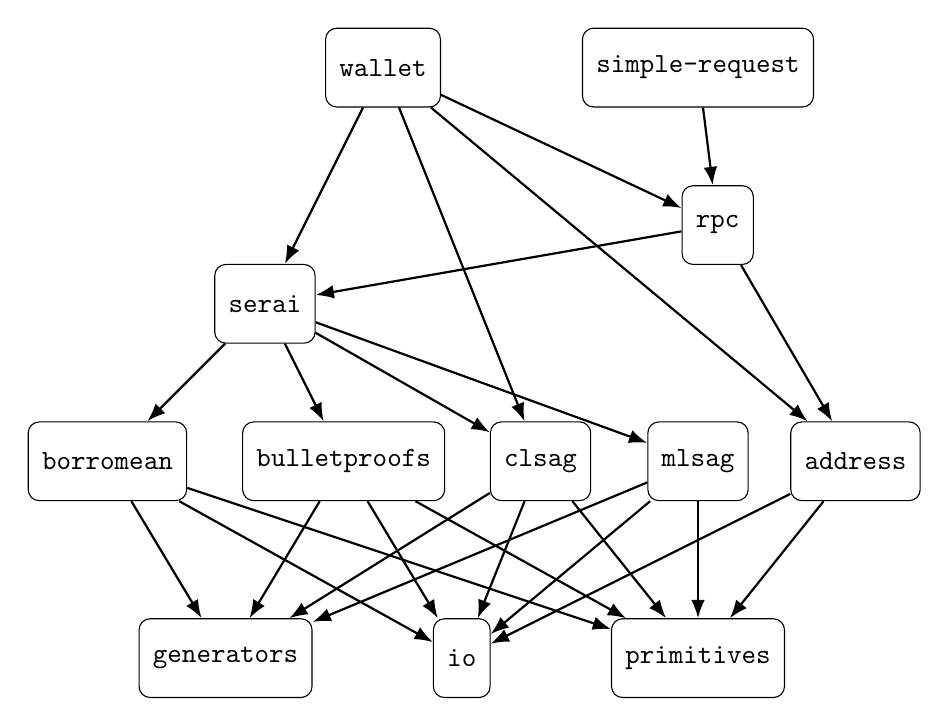
\begin{tikzpicture}[
    scale=1, % Ensure proper scaling
    every node/.style={draw, rectangle, rounded corners, minimum height=1cm, font=\ttfamily, inner sep=5pt, align=center}, % Rectangular nodes
    edge/.style={-{Latex}, thick}
]

% Manually normalized coordinates for a 10x7 aspect ratio
\node (wallet) at (4, 8.5) {wallet};
\node (simple-request) at (8, 8.5) {simple-request};
\node (rpc) at (8.25, 6.5) {rpc};
\node (serai) at (2.5, 5.5) {serai};
\node (address) at (10, 3.5) {address};
\node (mlsag) at (8, 3.5) {mlsag};
\node (clsag) at (6, 3.5) {clsag};
\node (bulletproofs) at (3.5, 3.5) {bulletproofs};
\node (borromean) at (0.5, 3.5) {borromean};
\node (io) at (5, 1) {io};
\node (generators) at (2, 1) {generators};
\node (primitives) at (8, 1) {primitives};

% Edges
\draw[edge] (wallet) -- (rpc);
\draw[edge] (wallet) -- (address);
\draw[edge] (wallet) -- (clsag);
\draw[edge] (wallet) -- (serai);
\draw[edge] (simple-request) -- (rpc);
\draw[edge] (rpc) -- (serai);
\draw[edge] (rpc) -- (address);
\draw[edge] (serai) -- (borromean);
\draw[edge] (serai) -- (bulletproofs);
\draw[edge] (serai) -- (clsag);
\draw[edge] (serai) -- (mlsag);
\draw[edge] (address) -- (io);
\draw[edge] (address) -- (primitives);
\draw[edge] (borromean) -- (io);
\draw[edge] (borromean) -- (generators);
\draw[edge] (borromean) -- (primitives);
\draw[edge] (bulletproofs) -- (io);
\draw[edge] (bulletproofs) -- (generators);
\draw[edge] (bulletproofs) -- (primitives);
\draw[edge] (clsag) -- (io);
\draw[edge] (clsag) -- (generators);
\draw[edge] (clsag) -- (primitives);
\draw[edge] (mlsag) -- (io);
\draw[edge] (mlsag) -- (generators);
\draw[edge] (mlsag) -- (primitives);

\end{tikzpicture}
\caption{The transitive reduction of the graph of crates and their dependencies. Not all edges corresponding to a direct dependency are displayed in a transitive reduction. For example, \texttt{monero-serai} depends directly on \texttt{monero-generators}, \texttt{monero-io}, and \texttt{monero-primitives}, but these edges are not explicitly displayed.}
\label{fig:transitive_reduced_dependency_graph}
\end{figure}

% \section{Functionality}

\section{Crates Overview}\label{sec:crate_summaries}

In this section, we describe each crate name, version, purpose, internal dependencies, and a brief description of crate structure. We use a breadth-first, top-down approach following Figure \ref{fig:transitive_reduced_dependency_graph}. Elements of public APIs (i.e.\ with the modifier \texttt{pub}) have names which are decorated \texttt{thusly}\textsuperscript{\textdagger}, and elements exposed at the crate level (i.e.\ with the modifier \texttt{pub(crate)}) have names which are decorated \texttt{thusly}\textsuperscript{$\Delta$}. We provide links throughout the document to corresponding glossary entries.

% The big itemize starts here

\begin{itemize}

 \item \gls{monero-wallet (v0.1.0)}
 \begin{itemize}
 \item Purpose: Handle all wallet functionality.
 \item Internal Dependencies:
 \begin{itemize}
 \item \gls{monero-address (v0.1.0)}\textsuperscript{\textdagger}
 \item \gls{monero-clsag (v0.1.0)}\textsuperscript{\textdagger}
 \item \gls{monero-rpc (v0.1.0)}\textsuperscript{\textdagger},
 \item \gls{monero-serai (v0.1.4-alpha)}\textsuperscript{\textdagger}
 \end{itemize}
 \item Structure: A standard library crate, with the corresponding entry point at  \gls{wallet-entry-point}.

 \item Tests at \gls{wallet-tests}.
 \item The \gls{monero-wallet (v0.1.0)} crate employs the following modules.
\begin{itemize}
\item \gls{decoys-module} handles decoy selection with a publicly exposed struct \texttt{OutputWithDecoys}.
\item \gls{extra-module}\textsuperscript{\textdagger} handles the \texttt{extra} field of a transaction.
\item \gls{output-module}\textsuperscript{$\Delta$} handles transaction outputs.
\item \gls{scan-module} handles transaction scanning.
\item \gls{send-module}\textsuperscript{\textdagger} handles sending transactions. This is a directory module, and contains the following file modules:
\begin{itemize}
\item \gls{eventuality-module} handles \gls{eventualities}.
\item \gls{send-multisig-module} handles sending threshold transactions.
\item \gls{send-tx-module} handles sending transactions.
\item \gls{send-tx-keys-module} handles keys for sending transactions.
\end{itemize}
\item \gls{view-pair-module} handles pairs of keys, where one is a public spend key, and the other is a private view key.
\end{itemize}

% Rigo added this
\end{itemize}


 \item \gls{monero-simple-request-rpc (v0.1.0)}
 \begin{itemize}
 \item Purpose: Default RPC to avoid external dependencies on, e.g.\ reqwest. Only used in dev dependencies.
 \item Internal Dependencies:
 \begin{itemize}
 \item \gls{monero-rpc (v0.1.0)}
 \end{itemize}
 \item Structure: A standard library crate,  with the corresponding entry point at  \gls{monero-simple-request-rpc-entry-point}.
\end{itemize}


 \item \gls{monero-rpc (v0.1.0)}
 \begin{itemize}
 \item Purpose: handle RPC calls for interacting on the Monero network.
 \item Internal Dependencies:
 \begin{itemize}
 \item \gls{monero-address (v0.1.0)}
 \item \gls{monero-serai (v0.1.4-alpha)}
 \end{itemize}
 \item Structure: A standard library crate, with the corresponding entry point at \gls{monero-rpc-entry-point}, employing no file or directory modules.
 \end{itemize}

\item \gls{monero-serai (v0.1.4-alpha)}
\begin{itemize}
\item Purpose: the overall transaction library.
\item Internal dependencies:
\begin{itemize}
\item \gls{monero-borromean (v0.1.0)}
\item \gls{monero-bulletproofs (v0.1.0)}
\item \gls{monero-clsag (v0.1.0)}
\item \gls{monero-generators (v0.4.0)}\textsuperscript{\textdagger}
\item \gls{monero-io (v0.1.0)}\textsuperscript{\textdagger}
\item \gls{monero-mlsag (v0.1.0)}
\item \gls{monero-primitives (v0.1.0)}\textsuperscript{\textdagger}
\end{itemize}
\item Structure: A standard library crate, with the corresponding entry point at \gls{monero-serai-entry-point}.
\begin{itemize}
\item File modules:
\begin{itemize}
\item \gls{block-module}\textsuperscript{\textdagger}
\item \gls{merkle-module}
\item \gls{ring-signatures-module}\textsuperscript{\textdagger}
\item \gls{ringct-module}\textsuperscript{\textdagger}
\item \gls{transaction-module}\textsuperscript{\textdagger}
\end{itemize}
\item Tests at \gls{monero-serai-tests}
\end{itemize}

% Rigo added this
\end{itemize}

\item \gls{monero-address (v0.1.0)}
\begin{itemize}
\item Purpose: handles Monero addresses.
\item Internal dependencies:
\begin{itemize}
\item \gls{monero-io (v0.1.0)}
\item \gls{monero-primitives (v0.1.0)}
\end{itemize}
\item Structure: A standard library crate, with the corresponding entry point at \gls{monero-address-entry-point}.
\begin{itemize}
\item File module: \gls{base58-module}.
\item Tests at \gls{address-tests}.
\end{itemize}
\end{itemize}



   \item \gls{monero-borromean (v0.1.0)}
   \begin{itemize}
   \item Purpose: Handles Borromean signatures and Borromean range proofs.
   \item Internal dependencies:
   \begin{itemize}
   \item \gls{monero-generators (v0.4.0)}
   \item \gls{monero-io (v0.1.0)}
   \item \gls{monero-primitives (v0.1.0)}
   \end{itemize}
   \item Structure: A standard library crate, with the corresponding entry point at \gls{borromean-entry-point}. Employs no modules, and untested.
   \end{itemize}

   \item \gls{monero-bulletproofs (v0.1.0)}
   \begin{itemize}
   \item Purpose: Handles original bulletproofs and bulletproofs plus.
   \item Internal dependencies:
   \begin{itemize}
   \item \gls{monero-generators (v0.4.0)}
   \item \gls{monero-io (v0.1.0)}
   \item \gls{monero-primitives (v0.1.0)}
   \end{itemize}
   \item Structure: A standard library crate, with the corresponding entry point at \gls{bulletproofs-entry-point}.
   \begin{itemize}
   \item File modules:
   \begin{itemize}
   \item \gls{bp-batch-verifier-module}\textsuperscript{$\Delta$}
   \item \gls{bp-core-module}\textsuperscript{$\Delta$}
   \item \gls{bp-point-vector-module}\textsuperscript{$\Delta$}
   \item \gls{bp-scalar-vector-module}\textsuperscript{$\Delta$}
   \end{itemize}
   \item Directory modules:
   \begin{itemize}
   \item \gls{bp-original-module}\textsuperscript{$\Delta$}
   \item \gls{bp-plus-module}\textsuperscript{$\Delta$}
   \end{itemize}
   \item Tests at \gls{bp-test-module}.
   \end{itemize}
   \end{itemize}



   \item \gls{monero-clsag (v0.1.0)}
   \begin{itemize}
   \item Purpose: Handles CLSAG ring signatures and a FROST-like thresholdization.
   \item Internal dependencies:
   \begin{itemize}
   \item \gls{monero-generators (v0.4.0)}
   \item \gls{monero-io (v0.1.0)}
   \item \gls{monero-primitives (v0.1.0)}
   \end{itemize}
   \item Structure: A standard library crate, with the corresponding entry point at \gls{monero-clsag-entry-point}.
   \begin{itemize}
   \item File module: \gls{clsag-multisig-module}.
   \item Tests: \gls{clsag-tests}
   \end{itemize}
   \end{itemize}

   \item \gls{monero-mlsag (v0.1.0)}
   \begin{itemize}
   \item Purpose: Handles MLSAG ring signatures.
   \item Internal dependencies:
   \begin{itemize}
   \item \gls{monero-generators (v0.4.0)}
   \item \gls{monero-io (v0.1.0)}
   \item \gls{monero-primitives (v0.1.0)}
   \end{itemize}
   \item Structure: A standard library crate with entry point at \gls{monero-mlsag-entry-point}. Employs no modules, and untested.
   \end{itemize}



 \item \gls{monero-primitives (v0.1.0)}
   \begin{itemize}
   \item Purpose: Handles Pedersen Commitments and Decoys.
   \item Internal dependencies:
   \begin{itemize}
   \item  \gls{monero-io (v0.1.0)}
   \item \gls{monero-generators (v0.4.0)}
   \end{itemize}
   \item Structure: A standard library crate with entry point at \gls{monero-primitives-entry-point}.
   \begin{itemize}

   \item File module at \gls{unreduced-scalar-module}.
   \item Tests at \gls{monero-primitives-tests}.
   \end{itemize}
   \end{itemize}



\item \gls{monero-generators (v0.4.0)}
   \begin{itemize}
   \item Purpose: Handles hashing data to elliptic curve group elements and all fixed generators used in Monero protocol computations.
   \item Internally dependent only on \gls{monero-io (v0.1.0)}.
   \item Structure: A standard library crate with entry point at \gls{monero-generators-entry-point}.
   \begin{itemize}

   \item File module at \gls{hash-to-point-module}.
   \item Tests at \gls{monero-generators-tests}
   \end{itemize}
   \end{itemize}

\item \gls{monero-io (v0.1.0)}
   \begin{itemize}
   \item Purpose: Handles reading and writing various data structures used in Monero protocol computations (e.g.\ bytes, scalars, group elements, lists whose entries are the same type).
   \item No internal dependencies.
   \item Structure: A standard library crate with entry point at \gls{monero-io-entry-point}. Employs neither modules nor tests.
\end{itemize}

% Rigo added this
\end{itemize}



%%%%%%%%%%%%%%%%%%%%%%%%%%%%%%%%%%%%%%%%%%%%%%%%%%%%%%%%%%%%%%%%%%%%%%%%%%%%%%%%
\section{\texttt{monero-io} (v0.1.0)}
The \texttt{monero-io} crate
(\path{networks/monero/io/src/lib.rs})
implements canonical serialization and deserialization routines
for various Monero protocol data types. It enforces strict
canonicalization where required by validating varint encoding,
scalar reduction, point encoding, and (optionally)
sub-group membership.

\begin{description}
\item[\texttt{varint} Encoding (\texttt{read\_varint})]
  Implemented at lines~133--151 .
  Uses a continuation-bit scheme to store a number in 7-bit chunks.
  The code rejects non-canonical encodings (leading zeros or overflow) and
  returns an error on malformed inputs.

\item[Scalar Serialization (\texttt{read\_scalar})]
  Implemented at lines~158--160.
  Reads a fixed 32-byte little-endian field element and ensures it is a
  canonical \texttt{curve25519-dalek} scalar, returning an
  \texttt{io::Error} otherwise.

\item[Point Serialization (\texttt{read\_point} /
      \texttt{read\_torsion\_free\_point})]
  Implemented at \\lines~179--185 and~187--193.
  \texttt{read\_point} calls \texttt{decompress\_point}
  (lines~172--176) to guarantee a unique, canonical encoding, while
  \texttt{read\_torsion\_free\_point} additionally verifies that the
  point lies in the prime-order subgroup.

\item[Vector Deserialization (\texttt{read\_array})]
  \label{item:read-array-lines208-214}
  At lines~208--214 the vector returned by \\\texttt{read\_raw\_vec} is
  guaranteed to have length~\texttt{N}; if not, \texttt{read\_raw\_vec}
  already returns an error and the closure is never invoked.  The
  subsequent \\\texttt{vec.try\_into().unwrap()} is therefore
  unreachable in practice and does not introduce a panic path.

\item[Length-Prefixed Vector Deserialization (\texttt{read\_vec})]
  \label{item:read-vec-lines216-219}
  At lines~216--219 a length prefix is read via \texttt{read\_varint},
  after which an \emph{empty} vector is created and elements are pushed
  one-by-one as long as the stream supplies valid items.
  Although the crate does not pre-allocate the reported size, a
  maliciously long (or infinite) stream can still lead to memory
  exhaustion.  Implementing an optional caller-supplied maximum length
  would mitigate this.

\end{description}

\noindent\textbf{Findings (monero-io v0.1.0):}
\begin{itemize}
  \item \textbf{Unbounded Length Acceptance}:
        \texttt{read\_vec} (lines 216–219) honours any length reported
        by \texttt{read\_varint}.  Exposing a configurable maximum
        element count is recommended.

  \item \textbf{Error Propagation \& Documented Panics}:
        Functions such as \texttt{varint\_len} and
        \texttt{write\_varint} will panic if the supplied value
        exceeds \texttt{u64::MAX}; this is documented behaviour.

  \item \textbf{Cofactor vs.\ Torsion Checks}:
        Callers that require prime-order points must use
        \texttt{read\_torsion\_free\_point}.
\end{itemize}

% \paragraph{Conclusion}
% Overall, \texttt{monero-io (v0.1.0)} adheres well to
% Monero’s canonical-encoding rules but would benefit
% from improved error handling in \texttt{read\_array}
% and \texttt{read\_vec} (lines~208--214
% and~216--219), as well as explicit bounds checks
% for large allocations. Replacing \texttt{unwrap()}
% with more robust handling will prevent panics when
% given malformed input. Finally, clarifying the difference
% between \texttt{read\_point} and
% \texttt{read\_torsion\_free\_point} ensures developers
% avoid accidental acceptance of torsioned or
% non-subgroup points.



%%%%%%%%%%%%%%%%%%%%%%%%%%%%%%%%%%%%%%%%%%%%%%%%%%%%%%%%%%%%%%%%%%%%%%%%%%%%%%%%
\section{\texttt{monero-generators} (v0.4.0)}

The \texttt{hash\_to\_point} function implements Monero's \texttt{hash\_to\_ec} operation to deterministically maps $32$ bytes to a point on the Ed25519 curve as in:

\begin{description}
\item[Input] \hfill
\begin{itemize}
\item Takes exactly $32$ bytes.  % https://github.com/serai-dex/serai/blob/48db06f901952b24bb38d7c7e256f798f08512cd/networks/monero/generators/src/hash_to_point.rs#L13
\end{itemize}

\item[Processing] \hfill
\begin{enumerate}
\item Performs \texttt{Keccak256} hash of input bytes.  % https://github.com/serai-dex/serai/blob/48db06f901952b24bb38d7c7e256f798f08512cd/networks/monero/generators/src/hash_to_point.rs#L17
\item Squares the hash result and doubles it to get value \texttt{v}.  % "
\item Computes intermediate values:
  \begin{itemize}
  \item $\texttt{w} = \texttt{v + 1}$.  % https://github.com/serai-dex/serai/blob/48db06f901952b24bb38d7c7e256f798f08512cd/networks/monero/generators/src/hash_to_point.rs#L18
  \item $\texttt{x} = \texttt{w}^2 - \texttt{A}^2v$ where $A = 486662$ (curve parameter).  % https://github.com/serai-dex/serai/blob/48db06f901952b24bb38d7c7e256f798f08512cd/networks/monero/generators/src/hash_to_point.rs#L15 and https://github.com/serai-dex/serai/blob/48db06f901952b24bb38d7c7e256f798f08512cd/networks/monero/generators/src/hash_to_point.rs#L19
  \item Calculates a partial $X$-coordinate through a series of field operations.  % https://github.com/serai-dex/serai/blob/48db06f901952b24bb38d7c7e256f798f08512cd/networks/monero/generators/src/hash_to_point.rs#L25-L33
  \end{itemize}
\item Derives $Y$-coordinate through:
  \begin{itemize}
  \item Calculates \texttt{y = w - x}.  % https://github.com/serai-dex/serai/blob/48db06f901952b24bb38d7c7e256f798f08512cd/networks/monero/generators/src/hash_to_point.rs#L36
  \item Sets sign bit based on zero checks.  % https://github.com/serai-dex/serai/blob/48db06f901952b24bb38d7c7e256f798f08512cd/networks/monero/generators/src/hash_to_point.rs#L37-L39
  \item Performs field inversions and multiplications to get final Y value.  % https://github.com/serai-dex/serai/blob/48db06f901952b24bb38d7c7e256f798f08512cd/networks/monero/generators/src/hash_to_point.rs#L41-L48
  \end{itemize}
\item Sets the high bit of byte $31$ based on calculated sign.  % https://github.com/serai-dex/serai/blob/48db06f901952b24bb38d7c7e256f798f08512cd/networks/monero/generators/src/hash_to_point.rs#L50
\end{enumerate}

\item[Output] \hfill
\begin{itemize}
\item Returns an EdwardsPoint in compressed $32$-byte format:  % https://github.com/serai-dex/serai/blob/48db06f901952b24bb38d7c7e256f798f08512cd/networks/monero/generators/src/hash_to_point.rs#L52
  \begin{itemize}
  \item Bytes $0$ through $30$: $Y$ coordinate.
  \item Byte $31$: Sign bit of $X$ coordinate (MSB format).  % https://github.com/serai-dex/serai/blob/48db06f901952b24bb38d7c7e256f798f08512cd/networks/monero/generators/src/hash_to_point.rs#L50
  \end{itemize}
\item Multiplies result by cofactor (8) to ensure point is in the prime-order subgroup.  % https://github.com/serai-dex/serai/blob/48db06f901952b24bb38d7c7e256f798f08512cd/networks/monero/generators/src/hash_to_point.rs#L52 (mul_by_cofactor)
\end{itemize}

\end{description}

The function uses the \texttt{FieldElement} type from \texttt{dalek-ff-group} for constant-time field arithmetic operations over the Ed25519 field of order $2^{255} - 19$.  All operations are performed in constant time as a mitigation against timing-based side-channel attacks.

\subsection{Operations}

The \texttt{monero-generators} crate provides generator points for Pedersen commitments and Bulletproofs in Monero as in:

\subsection{Core Generator}

\begin{description}
\item[Generation] \hfill \\
The base generator point $H$ is computed as in:
\begin{enumerate}
\item Take \texttt{ED25519\_BASEPOINT\_POINT} (the standard Ed25519 base point $G$).  % https://github.com/serai-dex/serai/blob/48db06f901952b24bb38d7c7e256f798f08512cd/networks/monero/generators/src/lib.rs#L10 and https://github.com/serai-dex/serai/blob/48db06f901952b24bb38d7c7e256f798f08512cd/networks/monero/generators/src/lib.rs#L29-L31
\item Compress it to $32$ bytes.  % https://github.com/serai-dex/serai/blob/48db06f901952b24bb38d7c7e256f798f08512cd/networks/monero/generators/src/lib.rs#L30
\item Compute \texttt{Keccak256} hash of these bytes.  % "
\item Map the hash to a curve point using \texttt{hash\_to\_point}.  % "
\item Multiply by the cofactor, $8$.  % https://github.com/serai-dex/serai/blob/48db06f901952b24bb38d7c7e256f798f08512cd/networks/monero/generators/src/lib.rs#L32
\end{enumerate}

\item[Powers Table] \hfill \\
Precomputes powers of H for efficient amount commitments as in:
\begin{itemize}
\item Creates array of $64$ points. The Rust implementation uses additive notation as do most CryptoNote-style protocols, so this is the vector\footnote{In the multiplicative notation more traditionally used in group theory, this is the vector $[H, H^{2}, H^{4}, ..., H^{2^{63}}]$.} $[H, 2H, 4H, \ldots, 2^{63}H]$.   % https://github.com/serai-dex/serai/blob/48db06f901952b24bb38d7c7e256f798f08512cd/networks/monero/generators/src/lib.rs#L35-L41
\item Each entry is double the previous entry.  % https://github.com/serai-dex/serai/blob/48db06f901952b24bb38d7c7e256f798f08512cd/networks/monero/generators/src/lib.rs#L38
\item Used for efficient decomposition of u64 amounts.  % https://github.com/serai-dex/serai/blob/48db06f901952b24bb38d7c7e256f798f08512cd/networks/monero/generators/src/lib.rs#L42-L48
\end{itemize}
\end{description}

\textbf{Potential Vulnerabilities and Recommendations:}
\begin{enumerate}
    \item \textbf{Use of \texttt{unwrap}}: Critical operations (e.g., field inversion, decompression) still employ \texttt{unwrap()} without explicit error handling.\
    \begin{quote}
     \textbf{Recommendation:} Replace \texttt{unwrap()} with \texttt{expect()} (with descriptive messages) or return a \texttt{Result} to mitigate unexpected panics.
    \end{quote}

    % \item \textbf{Keccak256 vs. SHA3-256}: The crate mirrors Monero’s choice to use Keccak256 rather than the finalized SHA3-256 standard.\\
    % \textbf{Recommendation:} Document this design decision clearly so maintainers understand the compatibility trade-offs and historical reasons.

    \item \textbf{Variable Reuse and Code Clarity}: Variables like \(\texttt{x}\) and \(\texttt{X}\), \(\texttt{y}\) and \(\texttt{Y}\) may cause confusion in the function’s local logic.
    \begin{quote}
     \textbf{Recommendation:} Consider inline comments clarifying each variable’s purpose to minimize confusion.
    \end{quote}
\end{enumerate}

\subsection{Bulletproofs Generator Vector Creation}

\begin{description}
\item[Constants] \hfill
\begin{itemize}
\item \texttt{MAX\_COMMITMENTS}: 16 (maximum provable commitments per range proof).  % https://github.com/serai-dex/serai/blob/48db06f901952b24bb38d7c7e256f798f08512cd/networks/monero/generators/src/lib.rs#L51
\item \texttt{COMMITMENT\_BITS}: 64 (bits per commitment value).  % https://github.com/serai-dex/serai/blob/48db06f901952b24bb38d7c7e256f798f08512cd/networks/monero/generators/src/lib.rs#L53
\item \texttt{MAX\_MN}: \texttt{MAX\_COMMITMENTS} * \texttt{COMMITMENT\_BITS} (total bits in proof).  % https://github.com/serai-dex/serai/blob/48db06f901952b24bb38d7c7e256f798f08512cd/networks/monero/generators/src/lib.rs#L72
\end{itemize}

\item[Generator Creation] \hfill \\
Takes a domain separation tag (\texttt{dst}) and produces two vectors of points: % https://github.com/serai-dex/serai/blob/48db06f901952b24bb38d7c7e256f798f08512cd/networks/monero/generators/src/lib.rs#L70
\begin{enumerate}
\item Create $\texttt{preimage} = H\texttt{.compress()} || \texttt{dst}$.  % https://github.com/serai-dex/serai/blob/48db06f901952b24bb38d7c7e256f798f08512cd/networks/monero/generators/src/lib.rs#L74-L75
\item For $i=0,\ldots,\texttt{MAX\_MN} - 1$: % https://github.com/serai-dex/serai/blob/48db06f901952b24bb38d7c7e256f798f08512cd/networks/monero/generators/src/lib.rs#L78-L89
  \begin{itemize}
  \item Let $j = 2*i$.  % https://github.com/serai-dex/serai/blob/48db06f901952b24bb38d7c7e256f798f08512cd/networks/monero/generators/src/lib.rs#L80
  \item $[i] = \texttt{hash\_to\_point}(\texttt{Keccak256}(\texttt{preimage} || \texttt{varint}(j)))$.  % https://github.com/serai-dex/serai/blob/48db06f901952b24bb38d7c7e256f798f08512cd/networks/monero/generators/src/lib.rs#L82-L84
  \item $G[i] = \texttt{hash\_to\_point}(\texttt{Keccak256}(\texttt{preimage} || \texttt{varint}(j+1)))$.  % https://github.com/serai-dex/serai/blob/48db06f901952b24bb38d7c7e256f798f08512cd/networks/monero/generators/src/lib.rs#L86-L88
  \end{itemize}
\end{enumerate}

\item[Output] \hfill \\
Returns \texttt{Generators} struct containing: % https://github.com/serai-dex/serai/blob/48db06f901952b24bb38d7c7e256f798f08512cd/networks/monero/generators/src/lib.rs#L58-L64
\begin{itemize}
\item G: Vector of \texttt{MAX\_MN} points for value commitments.  % https://github.com/serai-dex/serai/blob/48db06f901952b24bb38d7c7e256f798f08512cd/networks/monero/generators/src/lib.rs#L61
\item H: Vector of \texttt{MAX\_MN} points for mask commitments.  % https://github.com/serai-dex/serai/blob/48db06f901952b24bb38d7c7e256f798f08512cd/networks/monero/generators/src/lib.rs#L63
\end{itemize}
\end{description}

All operations maintain constant-time properties through:
\begin{itemize}
\item Use of \texttt{LazyLock} for thread-safe lazy initialization.  % https://github.com/serai-dex/serai/blob/48db06f901952b24bb38d7c7e256f798f08512cd/networks/monero/generators/src/lib.rs#L6 and https://github.com/serai-dex/serai/blob/48db06f901952b24bb38d7c7e256f798f08512cd/networks/monero/generators/src/lib.rs#L29 and https://github.com/serai-dex/serai/blob/48db06f901952b24bb38d7c7e256f798f08512cd/networks/monero/generators/src/lib.rs#L35
\item Constant-time point operations from \texttt{curve25519-dalek}.  % https://github.com/serai-dex/serai/blob/48db06f901952b24bb38d7c7e256f798f08512cd/networks/monero/generators/src/lib.rs#L10
\item Constant-time hash-to-point mapping.  % https://github.com/serai-dex/serai/blob/48db06f901952b24bb38d7c7e256f798f08512cd/networks/monero/generators/src/hash_to_point.rs#L1
\end{itemize}

% \textbf{Optimization and Usage Considerations:}
% \begin{itemize}
%     \item \textbf{Performance under Repeated Calls}: Generating vectors in a loop can be computationally expensive; caching or storing them in a static is recommended.
%     \item \textbf{Domain Separation}: The DST prevents collisions across different contexts, but careful documentation of the DST’s intended use is advised.
%     \item \textbf{Constant-Time Guarantees}: While scalar and point arithmetic are constant-time, the loop for generating \texttt{G}/\texttt{H} points depends on index-dependent hashing steps. Document any conditions under which data might become secret-dependent.
% \end{itemize}

% \subsection{Constant-Time and Thread-Safety Notes}
% \begin{itemize}
%     \item \textbf{Constant-Time Arithmetic}: Curve operations (additions, multiplications, etc.) are performed via \texttt{curve25519-dalek}’s constant-time primitives.
%     \item \textbf{Hashing and Varint Encoding}: These steps are not strictly constant-time, but typically operate on public indices or domain tags.
%     \item \textbf{LazyLock Safety}: Using \texttt{LazyLock} ensures single-threaded initialization of these vectors, preventing race conditions and providing a minor performance optimization when multiple threads need the same generator values.
% \end{itemize}

% \subsection{Test Coverage}
% \label{sec:monero-generators-tests}
% The crate includes extensive tests in \texttt{/generators/src/tests/mod.rs}, comparing:
% \begin{itemize}
%     \item \texttt{hash\_to\_point} outputs to official Monero test vectors, validating correctness across various inputs.
%     \item \texttt{check\_key} and generator logic against known reference data, ensuring \texttt{mul\_by\_cofactor} calls and compressed forms match expectations.
% \end{itemize}
% These tests help confirm the crate’s conformance to Monero’s cryptographic standards and maintain backward compatibility with its existing ecosystem.

% \subsection{Conclusion}
% The audit of the \texttt{monero-generators} crate reveals that while the implementation adheres to the core cryptographic requirements of the Monero protocol, several areas require attention to improve robustness and clarity:

% \begin{itemize}
%     \item \textbf{Error Handling:} Critical functions, especially in \texttt{hash\_to\_point}, rely on \texttt{unwrap} without explicit error management. Enhancing error reporting will mitigate unexpected panics.
%     \item \textbf{Documentation:} The complexity of the arithmetic operations and the assumptions made (e.g., on input size and DST validity) necessitate improved inline comments and function-level documentation.
%     \item \textbf{Efficiency and Exposure:} The current implementation’s iterative generator creation, while functionally correct, could be optimized for efficiency and secured by limiting the exposure of helper functions.
% \end{itemize}

% Overall, the findings highlight that the code is functionally correct and maintains constant-time operations, yet it would benefit significantly from improved error handling and documentation to prevent potential future issues. These recommendations are actionable and align with best practices for secure cryptographic implementations.



%%%%%%%%%%%%%%%%%%%%%%%%%%%%%%%%%%%%%%%%%%%%%%%%%%%%%%%%%%%%%%%%%%%%%%%%%%%%%%%%
\section{\texttt{monero-primitives} (v0.1.0)}

\subsection{Overview}
The \texttt{monero-primitives} crate provides the core cryptographic operations required by Monero's protocol.  The crate operates in both \texttt{std} and \texttt{no-std} environments, with certain optimizations available when \texttt{std} is enabled.

\subsection{Core Types}

\subsubsection{UnreducedScalar}
A structure representing an unreduced scalar value, primarily used to handle legacy Monero code sections where scalar reduction was not enforced: % https://github.com/serai-dex/serai/blob/48db06f901952b24bb38d7c7e256f798f08512cd/networks/monero/primitives/src/unreduced_scalar.rs#L22-L30

\begin{verbatim}
pub struct UnreducedScalar(pub [u8; 32]);
\end{verbatim}

Key operations:
\begin{itemize}
  \item \texttt{recover\_monero\_slide\_scalar}: Recovers the scalar that would have been incorrectly interpreted by Monero's \texttt{slide} function due to lack of reduction checks in Borromean range proofs. % https://github.com/serai-dex/serai/blob/48db06f901952b24bb38d7c7e256f798f08512cd/networks/monero/primitives/src/unreduced_scalar.rs#L110-L136
  \item \texttt{non\_adjacent\_form}: Computes the width-5 non-adjacent form (NAF) representation, intentionally matching Monero's potentially incorrect behavior. % https://github.com/serai-dex/serai/blob/48db06f901952b24bb38d7c7e256f798f08512cd/networks/monero/primitives/src/unreduced_scalar.rs#L52-L108
\end{itemize}

\subsubsection{Commitment}
Represents a transparent Pedersen commitment with the following structure: % https://github.com/serai-dex/serai/blob/48db06f901952b24bb38d7c7e256f798f08512cd/networks/monero/primitives/src/lib.rs#L80-L88

\begin{verbatim}
pub struct Commitment {
    pub mask: Scalar,
    pub amount: u64
}
\end{verbatim}

Operations:
\begin{itemize}
  \item \texttt{calculate}: Computes the Pedersen commitment point as $amount \cdot G + mask \cdot H$.  % https://github.com/serai-dex/serai/blob/48db06f901952b24bb38d7c7e256f798f08512cd/networks/monero/primitives/src/lib.rs#L107-L110
  \item \texttt{zero}: Creates a commitment to zero using a mask value of 1.  % https://github.com/serai-dex/serai/blob/48db06f901952b24bb38d7c7e256f798f08512cd/networks/monero/primitives/src/lib.rs#L97-L100
  \item Serialization and deserialization functionality.
\end{itemize}

\subsubsection{Decoys}
Manages ring signature data with the structure: % https://github.com/serai-dex/serai/blob/48db06f901952b24bb38d7c7e256f798f08512cd/networks/monero/primitives/src/lib.rs#L140-L146

\begin{verbatim}
pub struct Decoys {
    offsets: Vec<u64>,
    signer_index: u8,
    ring: Vec<[EdwardsPoint; 2]>
}
\end{verbatim}

Features:
\begin{itemize}
  \item Stores ring member positions as offsets from previous positions.  % https://github.com/serai-dex/serai/blob/48db06f901952b24bb38d7c7e256f798f08512cd/networks/monero/primitives/src/lib.rs#L184-L192
  \item Maintains key-commitment pairs for each ring member.  % https://github.com/serai-dex/serai/blob/48db06f901952b24bb38d7c7e256f798f08512cd/networks/monero/primitives/src/lib.rs#L145
  \item Provides access to the signer's position and ring members. % https://github.com/serai-dex/serai/blob/48db06f901952b24bb38d7c7e256f798f08512cd/networks/monero/primitives/src/lib.rs#L194-L207
\end{itemize}

\subsection{Core Operations}

\subsubsection{Hash Operations}
\begin{itemize}
  \item \texttt{keccak256}: Computes \texttt{Keccak256} hash of input data.  % https://github.com/serai-dex/serai/blob/48db06f901952b24bb38d7c7e256f798f08512cd/networks/monero/primitives/src/lib.rs#L62-L65
  \item \texttt{keccak256\_to\_scalar}: Maps input to a scalar via $\texttt{Keccak256}(\text{data}) \bmod \ell$, where $\ell$ is Ed25519's prime order. % https://github.com/serai-dex/serai/blob/48db06f901952b24bb38d7c7e256f798f08512cd/networks/monero/primitives/src/lib.rs#L67-L78
\end{itemize}

\subsubsection{Cached Computations}
When the \texttt{std} feature is enabled:
\begin{itemize}
  \item \texttt{INV\_EIGHT}: Caches $8^{-1} \bmod \ell$.  % https://github.com/serai-dex/serai/blob/48db06f901952b24bb38d7c7e256f798f08512cd/networks/monero/primitives/src/lib.rs#L29-L44
  \item \texttt{G\_PRECOMP}: Maintains precomputed tables for the Ed25519 base point. % https://github.com/serai-dex/serai/blob/48db06f901952b24bb38d7c7e256f798f08512cd/networks/monero/primitives/src/lib.rs#L46-L60
\end{itemize}

\subsection{Implementation Details}

\subsubsection{NAF Implementation}
% https://github.com/serai-dex/serai/blob/48db06f901952b24bb38d7c7e256f798f08512cd/networks/monero/primitives/src/unreduced_scalar.rs#L52-L105
\begin{itemize}
  \item Non-constant time operation, explicitly matching Monero's implementation.  % Documented at https://github.com/serai-dex/serai/blob/48db06f901952b24bb38d7c7e256f798f08512cd/networks/monero/primitives/src/unreduced_scalar.rs#L57
  \item Window size is fixed at $5$ bits.  % https://github.com/serai-dex/serai/blob/48db06f901952b24bb38d7c7e256f798f08512cd/networks/monero/primitives/src/unreduced_scalar.rs#L69
  \item Edge cases:
    \begin{itemize}
      \item Handles overflow beyond $256$ bits by truncating.  % https://github.com/serai-dex/serai/blob/48db06f901952b24bb38d7c7e256f798f08512cd/networks/monero/primitives/src/unreduced_scalar.rs#L70-L74
      \item Uses special carry propagation when the sum exceeds $15$ or the difference goes below $-15$.  % https://github.com/serai-dex/serai/blob/48db06f901952b24bb38d7c7e256f798f08512cd/networks/monero/primitives/src/unreduced_scalar.rs#L78-L101
      % \item Matches Monero's behavior even when cryptographically suboptimal.%
    \end{itemize}
\end{itemize}

The NAF computation in \texttt{non\_adjacent\_form} follows these steps:
\begin{enumerate}
  \item Convert input to a bit array.  % https://github.com/serai-dex/serai/blob/48db06f901952b24bb38d7c7e256f798f08512cd/networks/monero/primitives/src/unreduced_scalar.rs#L43-L50
  \item Process bits sequentially.  % https://github.com/serai-dex/serai/blob/48db06f901952b24bb38d7c7e256f798f08512cd/networks/monero/primitives/src/unreduced_scalar.rs#L61-L63
  \item For each non-zero bit: % https://github.com/serai-dex/serai/blob/48db06f901952b24bb38d7c7e256f798f08512cd/networks/monero/primitives/src/unreduced_scalar.rs#L66-L104
    \begin{itemize}
      \item Examine the next $5$ bits (window).  % https://github.com/serai-dex/serai/blob/48db06f901952b24bb38d7c7e256f798f08512cd/networks/monero/primitives/src/unreduced_scalar.rs#L69-L74
      \item Combine bits when sum $\leq 15$ or difference $\geq -15$.  % https://github.com/serai-dex/serai/blob/48db06f901952b24bb38d7c7e256f798f08512cd/networks/monero/primitives/src/unreduced_scalar.rs#L79-L84
      \item Handle carry propagation.  % https://github.com/serai-dex/serai/blob/48db06f901952b24bb38d7c7e256f798f08512cd/networks/monero/primitives/src/unreduced_scalar.rs#L91-L98
    \end{itemize}
\end{enumerate}

This intentionally matches Monero's implementation, including specific edge cases which may or may not be ``correct'' in contexts other than matching the Monero default wallet implementation.

\subsubsection{Scalar Recovery}
The \texttt{recover\_monero\_slide\_scalar} function:
\begin{itemize}
  \item Returns direct reduction if the high bit is not set.  % https://github.com/serai-dex/serai/blob/48db06f901952b24bb38d7c7e256f798f08512cd/networks/monero/primitives/src/unreduced_scalar.rs#L119-L124
  \item Otherwise reconstructs the scalar from its NAF representation.  % https://github.com/serai-dex/serai/blob/48db06f901952b24bb38d7c7e256f798f08512cd/networks/monero/primitives/src/unreduced_scalar.rs#L127-L134
  \item Uses precomputed odd scalars for efficiency.  % https://github.com/serai-dex/serai/blob/48db06f901952b24bb38d7c7e256f798f08512cd/networks/monero/primitives/src/unreduced_scalar.rs#L13-L20
\end{itemize}

\subsection{Security Considerations}

\subsubsection{Critical Assumptions}
\begin{itemize}
  \item A zero hash result in \texttt{keccak256\_to\_scalar} causes a panic.  % https://github.com/serai-dex/serai/blob/48db06f901952b24bb38d7c7e256f798f08512cd/networks/monero/primitives/src/lib.rs#L76
  \item \texttt{UnreducedScalar} operations do not guarantee constant-time execution.  % https://github.com/serai-dex/serai/blob/48db06f901952b24bb38d7c7e256f798f08512cd/networks/monero/primitives/src/lib.rs#L55-L60
  \item Commitment masking relies on the discrete logarithm assumption in the Ed25519 group.  % https://github.com/serai-dex/serai/blob/48db06f901952b24bb38d7c7e256f798f08512cd/networks/monero/primitives/src/lib.rs#L80-L88
\end{itemize}

\subsubsection{Implementation Notes}
\begin{itemize}
  \item \textbf{Serialization}:
    \begin{itemize}
      \item Uses custom formats, distinct from Monero protocol standards.  % https://github.com/serai-dex/serai/blob/48db06f901952b24bb38d7c7e256f798f08512cd/networks/monero/primitives/src/lib.rs#L112-L137 and https://github.com/serai-dex/serai/blob/48db06f901952b24bb38d7c7e256f798f08512cd/networks/monero/primitives/src/lib.rs#L209-L248
      \item Provides no backwards compatibility guarantees.  %
      % \item Limits \texttt{Decoys} serialization to Edwards points only.  % https://github.com/serai-dex/serai/blob/48db06f901952b24bb38d7c7e256f798f08512cd/networks/monero/primitives/src/lib.rs#L216-L223
    \end{itemize}
  \item \textbf{Memory Safety}:
    \begin{itemize}
      \item Implements \texttt{Zeroize} and \texttt{ZeroizeOnDrop} for sensitive data.  % eg. https://github.com/serai-dex/serai/blob/48db06f901952b24bb38d7c7e256f798f08512cd/networks/monero/primitives/src/lib.rs#L82
      \item Performs careful bounds checking when handling rings (anonymity sets/tuples). % https://github.com/serai-dex/serai/blob/48db06f901952b24bb38d7c7e256f798f08512cd/networks/monero/primitives/src/lib.rs#L165-L167
    \end{itemize}
  \item \textbf{Compatibility Choices}:
    \begin{itemize}
      \item Matches Monero behavior even when suboptimal.  % Documented at https://github.com/serai-dex/serai/blob/48db06f901952b24bb38d7c7e256f798f08512cd/networks/monero/primitives/src/unreduced_scalar.rs#L52-L57
      \item Preserves specific edge cases for protocol compatibility.  % https://github.com/serai-dex/serai/blob/48db06f901952b24bb38d7c7e256f798f08512cd/networks/monero/primitives/src/unreduced_scalar.rs#L119-L124
      \item Retains variable-time operations where Monero uses them. % Documented at https://github.com/serai-dex/serai/blob/48db06f901952b24bb38d7c7e256f798f08512cd/networks/monero/primitives/src/unreduced_scalar.rs#L52-L57
    \end{itemize}
\end{itemize}

\begin{itemize}
  \item Implements \texttt{Zeroize} and \texttt{ZeroizeOnDrop} for sensitive data.
  \item Matches Monero's behavior for compatibility, even if suboptimal.
  \item Employs crate-specific serialization formats, not the Monero protocol standard.
\end{itemize}

\subsection{Critical Findings}
\begin{enumerate}
    \item \textbf{Non-Adjacent Form (NAF) Vulnerability:} \\
    The \texttt{non\_adjacent\_form} function executes in variable time and is vulnerable to timing side-channel attacks.  This is documented.
    \begin{quote}
     \textbf{Recommendation:} Consider offering a constant-time alternative if used in secret-dependent contexts.
    \end{quote}

    % \item \textbf{Hash Function Choice:} \\
    % Keccak-256 is used in place of the finalized SHA3-256 standard, which may raise subtle compatibility and security concerns. \\
    % \textbf{Recommendation:} Clearly document the rationale for this choice along with its trade-offs.
\end{enumerate}

\subsection{Moderate Findings}
\begin{enumerate}
    \item \textbf{Inconsistent Error Handling:} \\
    The code uses a mix of \texttt{assert!}, \texttt{Option<T>}, and \texttt{io::Result<T>}, which can lead to unclear error propagation and unexpected termination.
    \begin{quote}
     \textbf{Recommendation:} Standardize on a uniform, \texttt{Result}-based error handling approach to provide consistent and contextual error reporting.
    \end{quote}
\end{enumerate}

\subsection{Neutral Findings}
\begin{enumerate}
    \item \textbf{Reachable Panic in Scalar Conversion:} \\
    The \texttt{keccak256\_to\_scalar} function uses an \texttt{assert!} that can panic if the resulting scalar equals zero.  This is a documented design decision because the probability of this occurring is \approx \frac{1}{2^{-252}} = \approx 2^{252}.
    \begin{quote}
     \textbf{Recommendation:} Replace the assertion with proper error propagation to safely handle unexpected inputs.
    \end{quote}
\end{enumerate}



%%%%%%%%%%%%%%%%%%%%%%%%%%%%%%%%%%%%%%%%%%%%%%%%%%%%%%%%%%%%%%%%%%%%%%%%%%%%%%%%
\section{\texttt{monero-rpc} (v0.1.0)}
\label{sec:monero-rpc-crate}

The \texttt{monero-rpc} crate provides abstractions for
communicating with a Monero daemon, retrieving various data (blocks, transactions,
fee estimates, \emph{etc.}), and publishing transactions.  The crate relies on data
structures from \texttt{monero-serai}, using them to parse and serialize Monero
primitives (such as transactions and blocks).  It offers a specialized trait for
decoy selection.

\subsection{Overview}
\label{sec:monero-rpc-overview}

The \texttt{monero-rpc} crate defines:

\begin{enumerate}
    \item \textbf{\texttt{RpcError}}: An enumeration capturing errors that may
    arise when performing RPC calls (see
    \S\ref{sec:monero-rpc-rpcerror}). % https://github.com/serai-dex/serai/blob/48db06f901952b24bb38d7c7e256f798f08512cd/networks/monero/rpc/src/lib.rs#L44-L74

    \item \textbf{\texttt{Rpc} trait}: The primary abstraction for interacting
    with a Monero daemon.  It defines a set of asynchronous methods for
    retrieving blocks, transactions, and other chain data, as well as
    publishing transactions (see \S\ref{sec:monero-rpc-rpc-trait}). % https://github.com/serai-dex/serai/blob/48db06f901952b24bb38d7c7e256f798f08512cd/networks/monero/rpc/src/lib.rs#L244-L252

    \item \textbf{\texttt{DecoyRpc} trait}: A higher-level trait extending the
    concept of retrieving outputs for constructing ring signatures (see
    \S\ref{sec:monero-rpc-decoy-rpc}). % https://github.com/serai-dex/serai/blob/48db06f901952b24bb38d7c7e256f798f08512cd/networks/monero/rpc/src/lib.rs#L1001-L1028 and https://github.com/serai-dex/serai/blob/48db06f901952b24bb38d7c7e256f798f08512cd/networks/monero/rpc/src/lib.rs#L1049-L1269

    \item \textbf{Various helpers and supporting items}, such as:
    \begin{itemize}
      \item \texttt{ScannableBlock}, bundling a \emph{Monero} block together
      with its non-miner transactions (in pruned form), plus metadata used when
      scanning outputs. % https://github.com/serai-dex/serai/blob/48db06f901952b24bb38d7c7e256f798f08512cd/networks/monero/rpc/src/lib.rs#L76-L87
      \item \texttt{FeeRate} and \texttt{FeePriority}, providing abstractions
      for Monero fee estimation. % https://github.com/serai-dex/serai/blob/48db06f901952b24bb38d7c7e256f798f08512cd/networks/monero/rpc/src/lib.rs#L76-L87
      \item Utility functions to parse certain specialized binary responses from
      a node, such as \texttt{get\_o\_indexes.bin}. % https://github.com/serai-dex/serai/blob/48db06f901952b24bb38d7c7e256f798f08512cd/networks/monero/rpc/src/lib.rs#L812-L999
    \end{itemize}
\end{enumerate}

Implementors of \texttt{Rpc} are expected to supply the low-level HTTP or
transport logic, including authentication if applicable.  The actual requests and
responses are shaped to match Monero’s JSON-RPC and specialized “binary”
endpoints.  This allows various backends (e.g., over Tor/i2p, local node,
dedicated HTTP crates) to be slotted in.

\subsection{\texttt{RpcError} Enumeration}
\label{sec:monero-rpc-rpcerror}

The \texttt{RpcError} enum defines all error conditions encountered by the RPC
layer: % https://github.com/serai-dex/serai/blob/48db06f901952b24bb38d7c7e256f798f08512cd/networks/monero/rpc/src/lib.rs#L43-L74

\begin{itemize}
    \item \textbf{\texttt{InternalError(String)}} --- Typically signals some
    logical problem unrelated to standard node replies (for instance,
    constructing a request with out-of-range parameters).

    \item \textbf{\texttt{ConnectionError(String)}} --- Indicates an inability
    to reach or properly communicate with the daemon (e.g.\ timeouts, malformed
    responses, or connectivity disruptions).

    \item \textbf{\texttt{InvalidNode(String)}} --- The remote node returned
    data not conforming to the Monero protocol, or otherwise gave impossible or
    contradictory information (suspecting a malicious or misconfigured node).

    \item \textbf{\texttt{TransactionsNotFound(Vec<[u8; 32]>)}} --- One or more
    requested transactions could not be retrieved by the node.

    \item \textbf{\texttt{PrunedTransaction}} --- A transaction was retrieved in
    a pruned form when unpruned data was required.  In the current code, pruned
    transactions are not considered usable for certain operations.

    \item \textbf{\texttt{InvalidTransaction([u8; 32])}} --- The node claims a
    transaction is valid, but it fails local parsing or verification.

    \item \textbf{\texttt{InvalidFee}} --- The fee returned by the node was
    nonsensical or out-of-range for safe usage.

    \item \textbf{\texttt{InvalidPriority}} --- The given fee priority could not
    be honored or mapped (e.g.\ out of the valid \texttt{1--4} range for
    Monero's known fee multipliers).
\end{itemize}

Such typed error handling allows the upper layers or other consumers of the
\texttt{monero-rpc} crate to correctly distinguish user-facing issues (like
\texttt{TransactionsNotFound}) from transport or malicious-node issues
(\texttt{ConnectionError} or \texttt{InvalidNode}).

\subsection{\texttt{Rpc} Trait}
\label{sec:monero-rpc-rpc-trait}

The \texttt{Rpc} trait is the centerpiece of the crate, defining the primary
asynchronous calls for interacting with a Monero daemon.  Its methods can be
broken into three categories: \emph{primitive calls}, \emph{block/transaction
retrieval}, and \emph{transaction publishing}. % https://github.com/serai-dex/serai/blob/48db06f901952b24bb38d7c7e256f798f08512cd/networks/monero/rpc/src/lib.rs#L244-L999

\subsection{\texttt{post}}
\label{sec:monero-rpc-rpc-trait-post}

\begin{verbatim}
fn post(
    &self,
    route: &str,
    body: Vec<u8>
) -> impl Future<Output = Result<Vec<u8>, RpcError>> + Send;
\end{verbatim}
% https://github.com/serai-dex/serai/blob/48db06f901952b24bb38d7c7e256f798f08512cd/networks/monero/rpc/src/lib.rs#L253-L260

At the lowest level, \texttt{post} takes an HTTP route string (e.g.:
\texttt{get\_transactions}) and a raw byte vector containing the request body.
It returns a future resolving to a \texttt{Result} with the raw byte vector for
the response (or an error).  Implementors must handle:

\begin{itemize}
    \item HTTP or HTTPS connections.
    \item Digest or basic authentication.
    \item Connection pooling or caching.
\end{itemize}

Nothing in \texttt{monero-rpc} enforces a particular method of connection;
\texttt{post} abstracts this detail away.

\subsection{\texttt{rpc\_call} and \texttt{json\_rpc\_call}}
\label{sec:monero-rpc-rpc-trait-jsonrpc}

\begin{verbatim}
fn rpc_call<Params: Serialize + Debug,
            Response: DeserializeOwned + Debug>(
    &self,
    route: &str,
    params: Option<Params>
) -> impl Future<Output = Result<Response, RpcError>> + Send;

fn json_rpc_call<Response: DeserializeOwned + Debug>(
    &self,
    method: &str,
    params: Option<Value>
) -> impl Future<Output = Result<Response, RpcError>> + Send;
\end{verbatim}
% https://github.com/serai-dex/serai/blob/48db06f901952b24bb38d7c7e256f798f08512cd/networks/monero/rpc/src/lib.rs#L262-L287 and https://github.com/serai-dex/serai/blob/48db06f901952b24bb38d7c7e256f798f08512cd/networks/monero/rpc/src/lib.rs#L289-L302

These two methods use \texttt{post} internally, providing:

\begin{enumerate}
    \item \texttt{rpc\_call}: For “raw” RPC calls, typically when a daemon
    endpoint does not follow the JSON-RPC 2.0 standard but instead uses
    POST-based JSON data (for example, \texttt{get\_transactions}).

    \item \texttt{json\_rpc\_call}: For endpoints explicitly requiring
    \texttt{json\_rpc} protocol usage (e.g. \texttt{get\_block\_header\_by\_height}).
    The parameters and method name are placed into the JSON-RPC structure, sent,
    and the result is deserialized back to a typed \texttt{Response}.
\end{enumerate}

Both automatically handle JSON deserialization into strongly typed Rust
structures.  If the response is malformed or the node returns an error-like
structure, \\ \texttt{RpcError::InvalidNode} or \texttt{RpcError::ConnectionError}
may be produced.

\subsection{\texttt{get\_height}, \texttt{get\_transactions}, and Block-Related Methods}

The crate includes convenience methods for:
\begin{itemize}
    \item \texttt{get\_height()}: Returns the current chain height (the number
    of blocks, with the genesis block counted as height $1$). % https://github.com/serai-dex/serai/blob/48db06f901952b24bb38d7c7e256f798f08512cd/networks/monero/rpc/src/lib.rs#L338-L354
    \item \texttt{get\_block}, \texttt{get\_block\_by\_number}, and
    \texttt{get\_block\_hash}: Retrieve and verify specific blocks, either by
    zero-indexed block number or by $32$-byte hash.  The code ensures the block’s
    serialized hash matches the node’s reported identifier, guarding against
    untrusted or corrupted data. % https://github.com/serai-dex/serai/blob/48db06f901952b24bb38d7c7e256f798f08512cd/networks/monero/rpc/src/lib.rs#L504-L584
    \item \texttt{get\_transactions} and \texttt{get\_pruned\_transactions}: % https://github.com/serai-dex/serai/blob/48db06f901952b24bb38d7c7e256f798f08512cd/networks/monero/rpc/src/lib.rs#L483
    Fetch zero or more transactions by their $32$-byte hash, verifying they match
    local expectations (checking the computed transaction hash).  Pruned or
    unpruned forms are selectively parsed via the relevant entry point.
    \item \texttt{get\_transaction} (unpruned) and
    \texttt{get\_pruned\_transaction}: Single-transaction convenience wrappers. % https://github.com/serai-dex/serai/blob/48db06f901952b24bb38d7c7e256f798f08512cd/networks/monero/rpc/src/lib.rs#L485-L494
\end{itemize}

Block retrieval can optionally return a \texttt{ScannableBlock}, packaging a
\texttt{Block} and its pruned non-coinbase transactions, allowing scanning for
RingCT outputs. % https://github.com/serai-dex/serai/blob/48db06f901952b24bb38d7c7e256f798f08512cd/networks/monero/rpc/src/lib.rs#L586-L655

\subsection{\texttt{publish\_transaction}}
\label{sec:monero-rpc-rpc-trait-publish}

\begin{verbatim}
fn publish_transaction(
    &self,
    tx: &Transaction
) -> impl Future<Output = Result<(), RpcError>> + Send;
\end{verbatim}
% https://github.com/serai-dex/serai/blob/48db06f901952b24bb38d7c7e256f798f08512cd/networks/monero/rpc/src/lib.rs#L742-L777

Publishes a \texttt{Transaction} to the network.  It leverages the
\texttt{send\_raw\_transaction} route (or equivalent) on the Monero daemon.
Should the daemon reject the transaction (for instance, if it conflicts with a
recently seen double spend), an appropriate \texttt{RpcError} is returned.

\subsection{\texttt{get\_fee\_rate}}
\label{sec:monero-rpc-rpc-trait-fee-estimate}

\begin{verbatim}
fn get_fee_rate(
    &self,
    priority: FeePriority
) -> impl Future<Output = Result<FeeRate, RpcError>> + Send;
\end{verbatim}
% https://github.com/serai-dex/serai/blob/48db06f901952b24bb38d7c7e256f798f08512cd/networks/monero/rpc/src/lib.rs#L675-L740

Requests fee estimates for a particular \texttt{FeePriority} (one of
\texttt{Unimportant}, \texttt{Normal}, \texttt{Elevated}, \texttt{Priority}, or
\texttt{Custom}).  Internally, it interprets the JSON response to obtain the fee
in “per-weight” units and a quantization mask.  The resulting \texttt{FeeRate}
structure:

\begin{itemize}
    \item \texttt{per\_weight}: The base fee per weight unit.
    \item \texttt{mask}: A mask used to round the final transaction fee upward.
\end{itemize}

The consumer can compute the final fee for a transaction based on the
transaction weight and this \texttt{FeeRate}.  If an unrecognized or invalid
priority is requested,\\ \texttt{RpcError::InvalidPriority} is raised.

\subsection{\texttt{generate\_blocks}}
\label{sec:monero-rpc-rpc-trait-generate-blocks}

While not part of a typical production Monero daemon (where block generation is
not done via RPC in mainnet environments), \texttt{generate\_blocks} is useful
in a local testing context (e.g.\ in a private regtest setup).  It creates
blocks, awarding the block reward to the specified \texttt{Address}.

\begin{verbatim}
fn generate_blocks<const ADDR_BYTES: u128>(
    &self,
    address: &Address<ADDR_BYTES>,
    block_count: usize
) -> impl Future<Output = Result<(Vec<[u8; 32]>, usize), RpcError>> + Send;
\end{verbatim}
% https://github.com/serai-dex/serai/blob/48db06f901952b24bb38d7c7e256f798f08512cd/networks/monero/rpc/src/lib.rs#L779-L810

This returns a list of the newly mined blocks’ hashes and the resulting height.

\subsection{\texttt{DecoyRpc} Trait}
\label{sec:monero-rpc-decoy-rpc}

The \texttt{DecoyRpc} trait extends the base RPC for selecting decoy outputs.
When constructing Monero transactions, ring signatures typically reference
random “decoy” outputs on-chain, enabling privacy.  \texttt{DecoyRpc} adds
specialized queries for zero-amount RingCT outputs:

\begin{itemize}
    \item \texttt{get\_output\_distribution\_end\_height()}: Reports the maximum
    block index used in the distribution.  Typically this equals the chain
    height. % https://github.com/serai-dex/serai/blob/48db06f901952b24bb38d7c7e256f798f08512cd/networks/monero/rpc/src/lib.rs#L1007-L1013
    \item \texttt{get\_output\_distribution(range: Range<usize>)}: Returns a
    vector of cumulative output counts for that block range.  By focusing on
    zero-amount outputs, it leverages the \texttt{get\_output\_distribution}
    endpoint. % https://github.com/serai-dex/serai/blob/48db06f901952b24bb38d7c7e256f798f08512cd/networks/monero/rpc/src/lib.rs#L1015-L1022
    \item \texttt{get\_outs(indexes: \&[u64])}: Fetches details for a batch of
    RingCT outputs, including the block height, unlocking status, compressed key
    ($\texttt{C}_i$), and the commitment (\texttt{mask}). % https://github.com/serai-dex/serai/blob/48db06f901952b24bb38d7c7e256f798f08512cd/networks/monero/rpc/src/lib.rs#L1024-L1028
    \item \texttt{get\_unlocked\_outputs(indexes, height, fingerprintable)}:
    Returns the subset of outputs that are actually unlocked by the node’s
    current chain state, or by a purely deterministic check (when
    \texttt{fingerprintable\_deterministic} is true).  This helps ensure
    decoys represent valid, spendable outputs from the node’s perspective. % https://github.com/serai-dex/serai/blob/48db06f901952b24bb38d7c7e256f798f08512cd/networks/monero/rpc/src/lib.rs#L1030-L1046
\end{itemize}

In typical usage, one might maintain a local database of zero-amount outputs
(built incrementally), but \texttt{DecoyRpc} allows direct on-demand retrieval
from a node if required.

\subsection{Supporting Types and Structures}
\label{sec:monero-rpc-supporting-types}

\subsubsection{\texttt{ScannableBlock}}
\label{sec:monero-rpc-supporting-types-scannableblock}

\begin{verbatim}
pub struct ScannableBlock {
    pub block: Block,
    pub transactions: Vec<Transaction<Pruned>>,
    pub output_index_for_first_ringct_output: Option<u64>,
}
\end{verbatim}
% https://github.com/serai-dex/serai/blob/48db06f901952b24bb38d7c7e256f798f08512cd/networks/monero/rpc/src/lib.rs#L76-L87

\texttt{ScannableBlock} encapsulates a fully read, unpruned coinbase
(\textit{miner}) transaction plus the pruned forms of other transactions, along
with an optional \\\texttt{output\_index\_for\_first\_ringct\_output}.  This index
helps to avoid repeated queries for the output index of every single
RingCT output in the block, which can be inefficient.

\subsubsection{\texttt{FeeRate}}
\label{sec:monero-rpc-supporting-types-feerate}

\begin{verbatim}
pub struct FeeRate {
    per_weight: u64,
    mask: u64,
}
\end{verbatim}
% https://github.com/serai-dex/serai/blob/48db06f901952b24bb38d7c7e256f798f08512cd/networks/monero/rpc/src/lib.rs#L89-L152

This data structure is an interpreted result from the node’s fee estimate.
The \\\texttt{FeeRate::calculate\_fee\_from\_weight} method performs final rounding:
\[
\text{fee} = \left\lceil \frac{\texttt{per\_weight}
             \times \texttt{tx\_weight}}{\texttt{mask}} \right\rceil
             \times \texttt{mask}.
\]
% https://github.com/serai-dex/serai/blob/48db06f901952b24bb38d7c7e256f798f08512cd/networks/monero/rpc/src/lib.rs#L138-L151

\subsubsection{\texttt{FeePriority}}
\label{sec:monero-rpc-supporting-types-feepriority}

\begin{verbatim}
pub enum FeePriority {
    Unimportant,
    Normal,
    Elevated,
    Priority,
    Custom { priority: u32 },
}
\end{verbatim}
% https://github.com/serai-dex/serai/blob/48db06f901952b24bb38d7c7e256f798f08512cd/networks/monero/rpc/src/lib.rs#L154-L173

Monero typically recognizes four distinct priority levels: “unimportant,”
“normal,” “elevated,” and “priority.”  Each internally maps to a numeric
multiplier for the base fee.  The \texttt{Custom} variant allows direct numeric
control, though the node might reject unknown or extreme values.

\subsection{Security Considerations}
\label{sec:monero-rpc-security}

\begin{enumerate}

    \item \textbf{Node Trust and Validation}: Since
    \texttt{monero-rpc} can operate on untrusted nodes, it attempts some
    validation (for example, verifying that a transaction’s hash matches the
    requested hash).  However, in general, the node is relied upon for essential
    data about chain state.  The \texttt{InvalidNode} error signals a mismatch
    from protocol expectations.
    % https://github.com/serai-dex/serai/blob/48db06f901952b24bb38d7c7e256f798f08512cd/networks/monero/rpc/src/lib.rs#L418-L428 for example.


    \item \textbf{Confidentiality of Queries}: Repeatedly querying the node
    about certain output indexes or unconfirmed transactions can leak usage
    patterns.  Future or external solutions may integrate local caches or batch
    requests to reduce fingerprinting.

    \item \textbf{Pruned Transactions}: If the node can only supply pruned
    data for certain legacy or low-mixin transactions, the library raises
    \texttt{RpcError::PrunedTransaction} if unpruned data is strictly required.
    Users must ensure they only proceed when they can meaningfully handle a
    pruned transaction (e.g.\ scanning coinbase outputs).
\end{enumerate}


\subsection{Findings}
\label{sec:monero-rpc-findings}

\begin{enumerate}
    \item \textbf{Unchecked Conversions and Potential Panics}:
    The codebase contains instances of unchecked type conversions and unwrapped operations (e.g., converting between \texttt{usize} and \texttt{u64} or \texttt{u32}) that can lead to runtime
    panics if given malicious or otherwise unexpected data.
    \begin{quote}
     \textbf{Recommendation:} Replace \texttt{unwrap()} calls with explicit error handling or use \texttt{expect()} with descriptive messages, ensuring domain assumptions are enforced.
    \end{quote}


    % \item \textbf{Error Handling Granularity}:
    % Several functions consolidate diverse errors into coarse error categories (e.g., mapping all
    % malformed responses to \texttt{InvalidNode}), making debugging more difficult.
    % \begin{itemize}
    %     \item \textbf{Recommendation:} Propagate errors with additional context and consider
    %     defining more granular error variants or dedicated error fields.
    % \end{itemize}

    % \item \textbf{Binary Protocol Parsing Issues}:
    % The custom parser for partially EPEE-formatted binary responses in \texttt{get\_o\_indexes.bin}
    % lacks thorough bounds checking and header/version validation. Although an \texttt{EPEE\_HEADER}
    % is defined, the implementation is minimal and might deviate from standard EPEE usage.
    % \begin{itemize}
    %     \item \textbf{Recommendation:} Modularize the parsing routines and enhance input validation
    %     (e.g., enforcing known lengths, checking for truncated data) to prevent potential memory or
    %     logic issues.
    % \end{itemize}

    \item \textbf{Limited Node Response Verification}:
    Verification of responses (e.g., in \\\texttt{get\_transactions}) primarily relies on hash
    comparisons with minimal structural checks. While this helps catch some invalid data, additional
    validation of response fields would improve security, such as:
    \begin{quote}
         \textbf{Recommendation:} Implement further integrity checks and stricter validation of node-supplied data, such as:
          \begin{itemize}
            \item Verifying that each returned transaction’s \emph{weight} matches the
                  byte-length supplied by the daemon.
            \item Ensuring every input’s key-image is 32\,B and—in pruned mode—that the
                  corresponding pseudo-output commitment is present.
            \item Rejecting blocks whose timestamp lies more than
                  \SI{2}{\hour} ahead/behind the local clock.
            \item Confirming that \texttt{extra} fields obey the length limits imposed
                  by consensus rules (e.g.\ bulletproof sizes, tx-public-key length).
          \end{itemize}
    \end{quote}

    \item \textbf{Timelock and Arithmetic Safety}:
    Unchecked arithmetic operations—especially those involving timelock values—could lead to
    overflows or logical errors. A \texttt{// TODO: ...} comment (e.g., referencing
    \texttt{github.com/serai-dex/serai/issues/104}) highlights the need for more robust handling of
    unusual timelock scenarios.
    \begin{quote}
         \textbf{Recommendation:} Use checked arithmetic operations and validate timelocks in boundary cases.
    \end{quote}

    % \item \textbf{Performance Considerations}:
    % Sequential asynchronous calls and a fixed batching limit (via \texttt{TXS\_PER\_REQUEST=100})
    % may limit performance. (The code references a Monero restriction that errors if more than 100
    % transactions are requested from a restricted RPC.)
    % \begin{itemize}
    %     \item \textbf{Recommendation:} Parallelize independent asynchronous calls and implement
    %     adaptive batching to accommodate varied node configurations.
    % \end{itemize}

    \item \textbf{Cryptographic Timing Considerations} (Informational)\\
      The RPC crate itself does not handle wallet private keys or other
      high-value secrets; equality checks currently compare only public data
      (hashes, commitments, points).  While side-channel risk is therefore low in
      today’s code, future extensions that compare secret-dependent values \emph{in
      place} must adopt constant-time routines (e.g.\
      \texttt{subtle::ConstantTimeEq}).
      \begin{quote}
        \textbf{Recommendation:}  Document this assumption clearly and integrate
        constant-time helpers if secret material is ever introduced.
      \end{quote}
\end{enumerate}

% \subsection{Summary of the \texttt{monero-rpc} Crate}
% \label{sec:monero-rpc-conclusion}

% The \texttt{monero-rpc} crate provides a clear, typed interface for interacting
% with Monero daemons, either trusted or untrusted.  By defining the \texttt{Rpc}
% trait, it ensures a uniform approach to retrieving, verifying, and publishing
% transactions, while the \texttt{DecoyRpc} trait extends it to fetch random ring
% outputs in a convenient, standardized manner.  This design integrates into
% higher layers of the \texttt{monero-serai} stack, making it easy to develop new
% functionality (e.g.\ bridging, multi-signature orchestrations, or custom
% wallets) in a modular and verifiable way.

% \subsection{Conclusion}
% \label{sec:monero-rpc-conclusion}

% The \texttt{monero-rpc} crate presents a well-structured interface for interacting with Monero daemons, balancing the needs for flexibility, security, and privacy. The implementation leverages strong cryptographic practices and careful zeroization of sensitive data. However, our audit has identified several areas for improvement:

% \begin{itemize}
%     \item Replace pervasive \texttt{unwrap()} calls with robust error handling to prevent runtime panics.
%     \item Enhance error propagation with more granular, context-rich messages.
%     \item Strengthen binary parsing routines with comprehensive bounds checking and header validation.
%     \item Expand verification of node responses to ensure complete data integrity.
%     \item Employ checked arithmetic in timelock computations to avoid overflows.
%     \item Optimize asynchronous patterns by parallelizing independent calls and adopting adaptive batching.
%     \item Implement constant-time comparisons for all sensitive cryptographic operations.
% \end{itemize}

% With these improvements, the \texttt{monero-rpc} crate will offer an even more robust and secure foundation for applications interfacing with the Monero network.



%%%%%%%%%%%%%%%%%%%%%%%%%%%%%%%%%%%%%%%%%%%%%%%%%%%%%%%%%%%%%%%%%%%%%%%%%%%%%%%%
\section{\texttt{monero-bulletproofs} (v0.1.0)}
\label{sec:monero-bulletproofs-impl}

The \texttt{monero-bulletproofs} crate implements both the original Bulletproofs range proof scheme and the newer Bulletproofs+ scheme for the Monero protocol.  The library is located within the Serai repository under \texttt{\small networks/monero/ringct/bulletproofs}.  Its purpose is to generate and verify range proofs over amounts in confidential transactions, ensuring that the amounts are in a valid range (specifically $[0, 2^{64})$) without revealing the amounts themselves.  Below is an overview of its structure, methods, and verification flow, referencing the relevant source files.

\subsection{Structure and Entry Points}
The crate exposes its main functionality via:
\begin{itemize}
    \item \texttt{Bulletproof}: An enum representing either the original Bulletproof or a Bulletproof+ proof. % https://github.com/serai-dex/serai/blob/48db06f901952b24bb38d7c7e256f798f08512cd/networks/monero/ringct/bulletproofs/src/lib.rs#L59-L69
    \item \texttt{prove} and \texttt{prove\_plus}: Functions that construct the respective Bulletproof or Bulletproof+ proofs for a list of commitments. % https://github.com/serai-dex/serai/blob/48db06f901952b24bb38d7c7e256f798f08512cd/networks/monero/ringct/bulletproofs/src/lib.rs#L108-L146
    \item \texttt{verify} and \texttt{batch\_verify}: Functions that verify these proofs, either in a standalone or batched manner. % https://github.com/serai-dex/serai/blob/48db06f901952b24bb38d7c7e256f798f08512cd/networks/monero/ringct/bulletproofs/src/lib.rs#L148-L173
\end{itemize}

Internally, the crate is separated into several modules:
\begin{itemize}
    \item \texttt{core}: Provides low-level operations such as multi-exponentiation routines and challenge product computation.
    \item \texttt{batch\_verifier}: Holds accumulators that enable batching multiple Bulletproof or Bulletproof+ verifications into a single multi-exponentiation.
    \item \texttt{original}: Implements the original Bulletproofs approach, including the inner-product proof (\texttt{IpProof}) used by \texttt{AggregateRangeProof}.
    \item \texttt{plus}: Implements Bulletproofs+ as described by the Monero project.  It includes the improved weighted inner product proof (\texttt{WipProof}) and the aggregated range proof mechanism that uses it.
    \item \texttt{scalar\_vector} and \texttt{point\_vector}: Utility types for vectors of \texttt{Scalar} and \\\texttt{EdwardsPoint}, offering safe indexing and algebraic operations.
    \item \texttt{tests}: Internal tests that validate correctness across both schemes, employing batched and single verifications.
\end{itemize}

\subsection{Range Proof Representation}
The top-level enum \texttt{Bulletproof} is:
\begin{itemize}
    \item \texttt{Original(OriginalProof)}: The classic Bulletproof structure using the original protocol design.
    \item \texttt{Plus(PlusProof)}: The Bulletproof+ structure, notably smaller and with a slightly different internal proving mechanism.
\end{itemize}

Each structure internally contains the group elements and scalars required for proof verification.  For instance, \texttt{OriginalProof} holds:
\begin{itemize}
    \item \texttt{(A, S, T1, T2)}: Points used in the range proof polynomial commitment.
    \item \texttt{tau\_x, mu, t\_hat}: Challenge-related scalars for the polynomial identity check.
    \item \texttt{ip}: An \texttt{IpProof} implementing the inner product argument.
\end{itemize}
% https://github.com/serai-dex/serai/blob/48db06f901952b24bb38d7c7e256f798f08512cd/networks/monero/ringct/bulletproofs/src/original/mod.rs#L29-L39

Likewise, \texttt{PlusProof} holds:
\begin{itemize}
    \item \texttt{A}: The aggregated vector commitment.
    \item \texttt{wip (WipProof)}: A specialized weighted inner product proof, the core cryptographic novelty of Bulletproofs+.
\end{itemize}
% https://github.com/serai-dex/serai/blob/48db06f901952b24bb38d7c7e256f798f08512cd/networks/monero/ringct/bulletproofs/src/plus/aggregate_range_proof.rs#L41-L47

\subsection{Aggregated Range Proof Generation}
Both Bulletproof and Bulletproof+ provide \emph{aggregated} proofs that combine multiple range proofs for multiple outputs into a single proof whose size grows only logarithmically in the number of outputs.  Each scheme follows a ``commit-and-challenge'' approach similar to standard Bulletproof protocols, but they differ in their choice of transcript hashing and the particular steps for the inner product argument.

\paragraph{Original Bulletproof (\texttt{original} module)}
The original code is in \texttt{original/mod.rs} and \texttt{original/inner\_product.rs}, closely mirroring the \textit{Bulletproofs} paper.  Key steps:
\begin{enumerate}
    \item \emph{Precomputation:} Generators \texttt{G} and \texttt{H} are allocated, one for each bit of each commitment.  The maximum number of commitments is specified by \texttt{\texttt{MAX\_COMMITMENTS}}. % MAX_COMMITMENTS imported at https://github.com/serai-dex/serai/blob/48db06f901952b24bb38d7c7e256f798f08512cd/networks/monero/ringct/bulletproofs/src/original/mod.rs#L9 and generators at https://github.com/serai-dex/serai/blob/48db06f901952b24bb38d7c7e256f798f08512cd/networks/monero/ringct/bulletproofs/src/original/mod.rs#L17 (generators generated in https://github.com/serai-dex/serai/blob/48db06f901952b24bb38d7c7e256f798f08512cd/networks/monero/ringct/bulletproofs/build.rs)
    \item \emph{Polynomial Commitments:} The protocol encodes bits of the amounts in vectors $(a_L, a_R)$, from which it forms commitments $(A, S)$. % https://github.com/serai-dex/serai/blob/48db06f901952b24bb38d7c7e256f798f08512cd/networks/monero/ringct/bulletproofs/src/original/mod.rs#L120-L166
    \item \emph{Challenges:} The code uses \texttt{Keccak256} (converted to a \texttt{Scalar} via \\\texttt{keccak256\_to\_scalar}) to derive random challenges $y, z, x$. % https://github.com/serai-dex/serai/blob/48db06f901952b24bb38d7c7e256f798f08512cd/networks/monero/ringct/bulletproofs/src/original/mod.rs#L65-L82 transcript_A_S for y,z challenges, transcript_T12 for x challenge
    \item \emph{Constrained Polynomial Identity:} The aggregator constructs $(T_1, T_2)$ to bind the polynomial terms, and merges everything with the challenge $x$ to produce $t_{\hat{}}$, $\tau_x$, and $\mu$. %
    \item \emph{Inner Product Proof:} The \texttt{IpProof} is generated by recursively splitting vectors in half and committing to partial inner products, storing the commitments $(L_i, R_i)$. % See https://github.com/serai-dex/serai/blob/48db06f901952b24bb38d7c7e256f798f08512cd/networks/monero/ringct/bulletproofs/src/original/mod.rs#L184-L222 for T1 and T2 commitments, transcript/challenge x, t_hat, tau_x, and mu.
\end{enumerate}

\paragraph{Bulletproof+ (\texttt{plus} module)}
Bulletproof+ is provided by the \texttt{plus/} folder, primarily in \texttt{weighted\_inner\_product.rs} and \texttt{aggregate\_range\_proof.rs}.  The official Monero code slightly alters the structure of the proof to reduce proof size, while still maintaining logarithmic size.  Notable elements:
\begin{enumerate}
    \item The \emph{Weighted Inner Product} (\texttt{WipStatement}) generalizes the classic inner product.  It incorporates certain transformations by weighting vectors with powers of $y$ and rearranging final group elements. % https://github.com/serai-dex/serai/blob/48db06f901952b24bb38d7c7e256f798f08512cd/networks/monero/ringct/bulletproofs/src/plus/weighted_inner_product.rs#L15-L28
    \item The \emph{Generators} are re-labeled for Monero's usage: \texttt{g\_bold} and \texttt{h\_bold} in code, though the actual roles are reversed (Monero uses $H$ as the value basepoint and $G$ for mask derivation). % https://github.com/serai-dex/serai/blob/48db06f901952b24bb38d7c7e256f798f08512cd/networks/monero/ringct/bulletproofs/src/plus/mod.rs#L25-L35
    \item Aggregation is performed similarly with powers of $z$ and $y$, but the final step uses a more efficient \texttt{WipProof}.
    \item The function \texttt{prove\_plus} sets up the aggregated statement, computes an $A$ commitment, then calls \texttt{WipStatement::prove} to produce the final weighted inner product proof. % See https://github.com/serai-dex/serai/blob/48db06f901952b24bb38d7c7e256f798f08512cd/networks/monero/ringct/bulletproofs/src/plus/aggregate_range_proof.rs#L186-L203 for z powers and https://github.com/serai-dex/serai/blob/48db06f901952b24bb38d7c7e256f798f08512cd/networks/monero/ringct/bulletproofs/src/plus/aggregate_range_proof.rs#L213-L234 for y powers and aggregation.
\end{enumerate}

At verification time, \texttt{aggregate\_range\_proof.rs} re-derives the same hashed challenges from the set of commitments and checks consistency with the \texttt{WipProof}.  As with the original proof, a batched approach merges all terms into a single multi-scalar multiplication check.

\subsection{Core Routines and Utilities}

\paragraph{\texttt{core/mod.rs}}
Contains low-level primitives:
\begin{itemize}
    \item \texttt{multiexp} and \texttt{multiexp\_vartime}: Perform (variable-time) multi-exponentiation to accumulate the proof checks. % https://github.com/serai-dex/serai/blob/48db06f901952b24bb38d7c7e256f798f08512cd/networks/monero/ringct/bulletproofs/src/core.rs#L31-L74
    \item \texttt{challenge\_products}: Generates the partial products of the challenges $(e_i, e_i^{-1})$ for the recursive proof steps, optimizing repeated multiplications. % https://github.com/serai-dex/serai/blob/48db06f901952b24bb38d7c7e256f798f08512cd/networks/monero/ringct/bulletproofs/src/core.rs#L50-L74
\end{itemize}

These functions are the primary means of combining scalar-point pairs for cryptographic checks throughout the library.

\paragraph{\texttt{batch\_verifier.rs}}
Implements the \texttt{BatchVerifier} structure, storing:
\begin{itemize}
    \item \texttt{original}: An accumulator for the original Bulletproof scheme. % https://github.com/serai-dex/serai/blob/48db06f901952b24bb38d7c7e256f798f08512cd/networks/monero/ringct/bulletproofs/src/batch_verifier.rs#L55-L62
    \item \texttt{plus}: An accumulator for Bulletproof+. % https://github.com/serai-dex/serai/blob/48db06f901952b24bb38d7c7e256f798f08512cd/networks/monero/ringct/bulletproofs/src/batch_verifier.rs#L64-L73
\end{itemize}

Each accumulator collects scalar multipliers for fixed and variable basepoints (respectively \texttt{G}, \texttt{H}, per-commitment bases, etc.).  Finally, \texttt{verify} executes a \emph{single} call to \texttt{vartime\_multiscalar\_mul} to confirm all queued proofs in batch.

\paragraph{\texttt{scalar\_vector.rs} and \texttt{point\_vector.rs}}
Define lightweight wrappers around \\ \texttt{Vec<Scalar>} and \texttt{Vec<EdwardsPoint>} to simplify:
\begin{itemize}
    \item Indexing with bounds checks (in debug mode). % https://github.com/serai-dex/serai/blob/48db06f901952b24bb38d7c7e256f798f08512cd/networks/monero/ringct/bulletproofs/src/scalar_vector.rs#L16-L26
    \item Element-wise operations: addition, subtraction, or multiplication on each vector element. % https://github.com/serai-dex/serai/blob/48db06f901952b24bb38d7c7e256f798f08512cd/networks/monero/ringct/bulletproofs/src/scalar_vector.rs#L28-L85
    \item Inner product computation: a straightforward $(\mathbf{a},\mathbf{b}) \mapsto \sum a_i b_i$. % https://github.com/serai-dex/serai/blob/48db06f901952b24bb38d7c7e256f798f08512cd/networks/monero/ringct/bulletproofs/src/scalar_vector.rs#L124-L130
\end{itemize}

These wrappers help maintain correctness by preventing mistakes in indexing or length mismatches between vectors.

\subsection{Transcript and Fiat--Shamir Challenges}
Throughout the protocol, challenges ($y, z, x, \dots$) are computed by hashing various group elements and scalars with \texttt{Keccak256}.  This is done via:
\begin{itemize}
    \item $\texttt{keccak256\_to\_scalar}(...)$: Converts a \texttt{Keccak256} hash into a \texttt{Scalar}. % https://github.com/serai-dex/serai/blob/48db06f901952b24bb38d7c7e256f798f08512cd/networks/monero/ringct/bulletproofs/src/plus/transcript.rs#L13-L17
    \item Combined with domain separators and partial transcripts (e.g.\ $\texttt{A}$, $\texttt{S}$, $\texttt{T1}$, $\texttt{T2}$ in the original scheme). % https://github.com/serai-dex/serai/blob/48db06f901952b24bb38d7c7e256f798f08512cd/networks/monero/ringct/bulletproofs/src/plus/transcript.rs#L8-L11
\end{itemize}

In \texttt{plus/transcript.rs}, Bulletproof+ uses an additional domain separation constant \verb|bulletproof_plus_transcript|, plus Monero's \texttt{hash\_to\_point} trick, though its necessity is not entirely clear from the code.

\subsection{Security Observations}
\begin{itemize}
    \item \emph{Cofactor clearing}: By multiplying all external inputs (\texttt{EdwardsPoint} commitments) by \texttt{INV\_EIGHT} then re-multiplying by 8, the code ensures those points lie in the primary subgroup.  This is critical to avoid torsion-based forgeries. % See https://github.com/serai-dex/serai/blob/48db06f901952b24bb38d7c7e256f798f08512cd/networks/monero/ringct/bulletproofs/src/original/mod.rs#L61-L62 for INV_EIGHT multiplication and https://github.com/serai-dex/serai/blob/48db06f901952b24bb38d7c7e256f798f08512cd/networks/monero/ringct/bulletproofs/src/batch_verifier.rs#L23-L53 for is_identity check.
    \item \emph{Batch verification correctness}: Accumulated scalars and points are carefully updated to ensure the final check equals the identity only if all aggregated proofs are valid.  If any proof is malformed, the final multi-exponentiation will yield a non-identity point. % See latter reference above.
    \item \emph{Randomness and transcript:} The crate depends on externally provided randomness (via \texttt{rand\_core} or through \texttt{OsRng} in tests).  The Fiat--Shamir heuristic is used for non-interactive challenge derivation. % See https://github.com/serai-dex/serai/blob/48db06f901952b24bb38d7c7e256f798f08512cd/networks/monero/ringct/bulletproofs/src/plus/transcript.rs for Fiat-Shamir.
\end{itemize}

\subsection{Findings}

\begin{enumerate}
    \item \textbf{Transcript Construction and Domain Separation:}\\
    The code (e.g.\ \texttt{plus/transcript.rs} lines \texttt{8--17} and \texttt{transcript\_A\_B} in \\\texttt{weighted\_inner\_product.rs} lines \texttt{247--269}) employs a static domain-separation constant derived via \texttt{hash\_to\_point}. Although functionally correct, the inline documentation does not explicitly clarify how this constant binds challenges to specific protocol parameters or commit to all relevant data (e.g.\ original basepoints).
    \begin{quote}
        \textbf{Recommendation:} Expand inline comments or code documentation to explain each parameter included in the transcript, referencing Monero’s recommended domain separation. Where possible, incorporate additional references (like basepoints or block-specific tags) to reduce the risk of cross-protocol collisions.
    \end{quote}

    \item \textbf{Error Handling and Unchecked Conversions:}\\
    Several functions still rely on \texttt{unwrap()}, but the
    uses in \texttt{lib.rs} lines~108–146 (\texttt{prove}) come \emph{after} the witness has
    already been validated (lines~108–113).
    Because the two validation stages are wholly internal to the crate, these panics should be
    unreachable in practice.  The current structure is therefore sound, though slightly
    duplicitous.

    \begin{quote}
      \textbf{Recommendation:} Consolidate the two validation paths (witness checks and the
      subsequent assertions) or replace the remaining \texttt{unwrap()}s with explicit
      error-propagation helpers such as \texttt{expect("invariant violated")}.  Either approach
      would preserve today’s safety guarantee while making the intended invariant clearer to
      future maintainers.
    \end{quote}

    \item \textbf{Cofactor Clearing and Documentation Consistency:}\\
    The code correctly multiplies external inputs by \texttt{INV\_EIGHT} and compensates by multiplying by \texttt{8} later (e.g.\ \texttt{original/mod.rs} lines \texttt{61--62} and \texttt{batch\_verifier.rs} lines \texttt{23--53}). However, the comments explaining why this step eliminates torsion-based forgeries vary in detail across modules.
    \begin{quote}
        \textbf{Recommendation:} Standardize these comments to note that cofactor clearing ensures points lie in the primary subgroup. Reference lines \texttt{61--62} in \texttt{original/mod.rs} from the vantage of best practices recommended in cryptographic literature (e.g.\ the rationale behind multiplying by the cofactor).
    \end{quote}

    \item \textbf{Variable-Time Operations:}\\
    The crate uses \texttt{multiexp\_vartime} for public data, which is acceptable as long as it is never called with secret-dependent scalars. For instance, see \texttt{core.rs} lines \texttt{50--74} and references in \texttt{plus/weighted\_inner\_product.rs} lines \texttt{416--435}.
    \begin{quote}
        \textbf{Recommendation:} Audit each call to \texttt{multiexp\_vartime} to ensure it cannot be reached with secret values. If any scalar is secret, switch to a constant-time alternative or document precisely why variable time is safe (e.g.\ purely public aggregator data).
    \end{quote}

    % \item \textbf{Prover Logic and Recursive Inner Product Loop:}\\
    % Both the original and plus schemes rely on a recursive splitting of vectors in half. For example, \texttt{original/inner\_product.rs} lines \texttt{195--231} handle splitting for the \texttt{IpProof} and \texttt{plus/weighted\_inner\_product.rs} lines \texttt{304--353} do similarly for \texttt{WipProof}. While the code is correct, it assumes inputs are padded to a power-of-two length. If the user passes a vector of scalars or points that is not padded, the code attempts to do so automatically without robust checks.
    % \begin{quote}
    %     \textbf{Recommendation:} Add explicit assertions or better documentation clarifying the padding. For instance, note at the start of \texttt{prove()} that the code extends vectors to the nearest power of two, and confirm that the user is aware of any trailing zero elements introduced.
    % \end{quote}
\end{enumerate}



%%%%%%%%%%%%%%%%%%%%%%%%%%%%%%%%%%%%%%%%%%%%%%%%%%%%%%%%%%%%%%%%%%%%%%%%%%%%%%%%
\section{\texttt{monero-address} (v0.1.0)}

\subsection{Purpose}

The \texttt{monero-address} crate provides functionality for handling Monero addresses, including standard, subaddress, integrated, and featured addresses.  It also supports encoding and decoding Monero addresses in \texttt{base58Check} format.

\subsection{Internal Dependencies}

\begin{itemize}
    \item \texttt{monero-io (v0.1.0)}.
    \item \texttt{monero-primitives (v0.1.0)}.
\end{itemize}

\subsection{Structure}

A standard library crate, with the corresponding entry point at \path{/wallet/address/src/lib.rs}.

\begin{itemize}
    \item \texttt{base58Check} module.
    \item Tests at \path{/wallet/address/src/tests.rs}.
\end{itemize}

\subsection{Functionality}

The \texttt{monero-address} crate defines several types of Monero addresses and provides encoding, decoding, and validation functionality.

\paragraph{Address Types}

The \texttt{monero-address} crate defines the following address types.

\begin{itemize}
    \item \textbf{Legacy:} A standard Monero address (public spend and view keys).
    \item \textbf{Legacy Integrated:} A legacy address with an embedded $8$-byte payment ID.
    \item \textbf{Subaddress:} A derived address that allows the receiver to differentiate sources of funds.
    \item \textbf{Featured Address:} An extended address format supporting subaddresses, embedded payment IDs, and a guarantee against the burning bug.
\end{itemize}
% https://github.com/serai-dex/serai/blob/48db06f901952b24bb38d7c7e256f798f08512cd/networks/monero/wallet/address/src/lib.rs#L24-L58

Each address type is represented using the \texttt{AddressType} enum, which provides methods for checking whether an address is a subaddress, retrieving its embedded payment ID, and determining if it is guaranteed. % https://github.com/serai-dex/serai/blob/48db06f901952b24bb38d7c7e256f798f08512cd/networks/monero/wallet/address/src/lib.rs#L60-L86

\paragraph{Network Identification}

The \texttt{Network} enum defines three possible Monero network types.

\begin{itemize}
    \item \textbf{Mainnet:} The primary Monero blockchain.
    \item \textbf{Stagenet:} A staging network with the same rules as mainnet, used for testing.
    \item \textbf{Testnet:} A network used to test new features before they are deployed.
\end{itemize}
% https://github.com/serai-dex/serai/blob/48db06f901952b24bb38d7c7e256f798f08512cd/networks/monero/wallet/address/src/lib.rs#L186-L199

Each network is associated with specific address prefix bytes to distinguish them from each other. % https://github.com/serai-dex/serai/blob/48db06f901952b24bb38d7c7e256f798f08512cd/networks/monero/wallet/address/src/lib.rs#L339-L347

\paragraph{\texttt{base58Check} Encoding and Decoding}

The \texttt{base58Check} module implements \\ \texttt{base58Check} encoding and decoding, ensuring that Monero addresses include a checksum for error detection. % https://github.com/serai-dex/serai/blob/48db06f901952b24bb38d7c7e256f798f08512cd/networks/monero/wallet/address/src/base58check.rs#L86-L106

\begin{itemize}
    \item \texttt{encode}: Encodes a byte array into \texttt{base58Check} format.
    \item \texttt{decode}: Decodes a \texttt{base58Check} string into raw bytes.
    \item \texttt{encode\_check}: Computes a checksum and encodes a byte array into \texttt{base58Check}.
    \item \texttt{decode\_check}: Decodes a \texttt{base58Check} string and verifies its checksum.
\end{itemize}

% \paragraph{Potential \texttt{unwrap()} Panics in Base58Check}
% Within \path{/wallet/address/src/base58check.rs}, code such as:
% \begin{verbatim}
% let mut val = ...;
% chunk_str[i] = ALPHABET[usize::try_from(val % ALPHABET_LEN).expect("...")]
%   as char;
% \end{verbatim}
% and in \texttt{decode} or \texttt{decode\_check}, can panic if \texttt{val} is out of bounds (though the logic attempts to ensure it is not). This constitutes a \textbf{Medium-Risk} possibility for adversarial inputs.

\paragraph{Address Parsing and Generation}

Monero addresses can be created from public spend and view keys, or parsed from strings. % https://github.com/serai-dex/serai/blob/48db06f901952b24bb38d7c7e256f798f08512cd/networks/monero/wallet/address/src/lib.rs#L401-L461

\begin{itemize}
    \item \texttt{MoneroAddress::new}: Creates a new Monero address given a network, address type, and key pair.
    \item \texttt{MoneroAddress::from\_str}: Parses an address string for a given network.
    \item \texttt{MoneroAddress::from\_str\_with\_unchecked\_network}: Parses an address string without verifying the network.
    \item \texttt{MoneroAddress::to\_string}: Serializes an address to a \texttt{base58Check}-encoded string.
\end{itemize}

\paragraph{Address Validation}

The crate ensures that parsed addresses meet the expected format. % https://github.com/serai-dex/serai/blob/48db06f901952b24bb38d7c7e256f798f08512cd/networks/monero/wallet/address/src/lib.rs#L419-L440

\begin{itemize}
    \item \textbf{Length validation:} Ensures addresses are the correct length based on their type.
    \item \textbf{Checksum verification:} Ensures that decoded addresses pass the \texttt{base58Check} validation.
    \item \textbf{Key validation:} Ensures that the spend and view keys are valid Edwards25519 points.
\end{itemize}

\subsection{Serialization Details}

The \texttt{monero-address} crate serializes addresses into a compact binary format before encoding them into \texttt{base58Check}.  The serialization structure is as follows. % https://github.com/serai-dex/serai/blob/48db06f901952b24bb38d7c7e256f798f08512cd/networks/monero/wallet/address/src/lib.rs#L381-L399

\begin{enumerate}
    \item \textbf{Network Byte:} A single byte indicating the network and address type.
    \item \textbf{Spend Key:} A $32$-byte compressed Edwards25519 public key.
    \item \textbf{View Key:} A $32$-byte compressed Edwards25519 public key.
    \item \textbf{Optional Fields:}
    \begin{itemize}
        \item \textbf{Integrated Payment ID:} An $8$-byte payment ID (only for integrated addresses).
        \item \textbf{Feature Flags:} A variable-length integer encoding subaddress, payment ID, and guarantee status.
    \end{itemize}
    \item \textbf{Checksum:} A $4$-byte \texttt{Keccak256} hash of the serialized data.
\end{enumerate}
% See https://github.com/serai-dex/serai/blob/48db06f901952b24bb38d7c7e256f798f08512cd/networks/monero/wallet/address/src/lib.rs#L381-L399 and https://github.com/serai-dex/serai/blob/48db06f901952b24bb38d7c7e256f798f08512cd/networks/monero/wallet/address/src/base58check.rs#L86-L91 for checksum details.

\subsection{Testing}

The \texttt{monero-address} crate includes comprehensive tests to validate the correctness of its encoding, decoding, and parsing functions. % https://github.com/serai-dex/serai/blob/48db06f901952b24bb38d7c7e256f798f08512cd/networks/monero/wallet/address/src/tests.rs

\begin{itemize}
    \item \textbf{Base58Check Encoding Tests:} Ensures that encoded addresses correctly round-trip through decoding.
    \item \textbf{Standard Address Tests:} Validates correct parsing and serialization of standard Monero addresses.
    \item \textbf{Integrated Address Tests:} Ensures proper handling of embedded payment IDs.
    \item \textbf{Subaddress Tests:} Validates the ability to generate and recognize subaddresses.
    \item \textbf{Featured Address Tests:} Ensures correct parsing and serialization of extended features.
    \item \textbf{Vector-Based Tests:} Uses predefined address vectors to ensure consistency with expected values.
\end{itemize}

The test suite ensures that all address types are handled correctly and provides coverage for both expected and edge cases.

\subsection{Findings}
\begin{enumerate}
    \item \textbf{Use of \texttt{expect} in Internal Helpers (Informational)}\\
    Both \texttt{encoded\_len\_for\_bytes} and the
    \texttt{encode}/\texttt{decode} loops employ
    \texttt{expect()} on conversions that are \emph{provably} in-range once
    Rust’s minimum pointer width (\(\ge 16\) bits) is assumed.  Because the
    value being indexed is reduced modulo~58 on every iteration, an
    out-of-bounds index is unreachable.  Consequently, no adversarial input can
    trigger a panic on supported platforms.  No code change recommended.

    % \item \textbf{Documentation Gaps on \texttt{Featured} Varint Construction (Low Risk)}\\
    % Although the code references the subaddress/payment‐ID/guaranteed bits in inline comments, the original audit text did not mention it in detail. Lack of external documentation might confuse new developers.\\
    % \textbf{Recommendation:} Expand code‐level docs (especially around lines \textit{\texttt{160--220}} in \texttt{lib.rs}) to highlight the security implications of storing multiple flags in a varint, referencing any relevant design rationale.

\end{enumerate}



%%%%%%%%%%%%%%%%%%%%%%%%%%%%%%%%%%%%%%%%%%%%%%%%%%%%%%%%%%%%%%%%%%%%%%%%%%%%%%%%
\section{\texttt{monero-clsag} (v0.1.0)}
The \texttt{monero-clsag} crate implements Compact Linkable Spontaneous Anonymous Group (CLSAG) signatures and provides a FROST-inspired threshold signing mechanism.
The implementation consists of two main components:

\subsection{Core CLSAG Implementation}
\begin{description}
\item[\texttt{ClsagContext}] \hfill \\ % https://github.com/serai-dex/serai/blob/48db06f901952b24bb38d7c7e256f798f08512cd/networks/monero/ringct/clsag/src/lib.rs#L65-L72
Holds the context needed for signing:
\begin{itemize}
\item A commitment opening (mask and amount)
\item Selected decoy positions and ring
\end{itemize}

\item[\texttt{Clsag} Signature] \hfill \\ % https://github.com/serai-dex/serai/blob/48db06f901952b24bb38d7c7e256f798f08512cd/networks/monero/ringct/clsag/src/lib.rs#L222-L231
A signature consisting of:
\begin{itemize}
\item D: Difference of commitment randomness scaling the key image generator
\item s: Vector of responses for each ring member
\item c1: First challenge in the ring
\end{itemize}

\item[Core Algorithm] \hfill \\ % https://github.com/serai-dex/serai/blob/48db06f901952b24bb38d7c7e256f798f08512cd/networks/monero/ringct/clsag/src/lib.rs#L96-L220
The core signing/verification algorithm:
\begin{enumerate}
\item Takes ring members, key image I, pseudo-out P, and message m
\item For signing:
  \begin{itemize}
  \item Generates random nonces for the real signer
  \item Computes the key image generator from the public key
  \item Calculates initial commitments A and AH
  \end{itemize}
\item For both signing and verifying:
  \begin{itemize}
  \item Computes challenges using \texttt{Keccak256}
  \item Performs ring calculations over the Ed25519 group
  \item Validates signature components
  \end{itemize}
\end{enumerate}
\end{description}

\subsection{FROST-Inspired Threshold Signing}
\begin{description}
\item[\texttt{ClsagMultisig}] \hfill \\ % https://github.com/serai-dex/serai/blob/48db06f901952b24bb38d7c7e256f798f08512cd/networks/monero/ringct/clsag/src/multisig.rs#L115-L137
Implements threshold signing for CLSAG:
\begin{itemize}
\item Uses FROST key generation and coordination
\item Extends CLSAG to support threshold key images
\item Preserves CLSAG's linkability property
\end{itemize}

\item[Key Components] \hfill  % See https://github.com/serai-dex/serai/blob/48db06f901952b24bb38d7c7e256f798f08512cd/networks/monero/ringct/clsag/src/multisig.rs#L57-L68 and https://github.com/serai-dex/serai/blob/48db06f901952b24bb38d7c7e256f798f08512cd/networks/monero/ringct/clsag/src/multisig.rs#L86-L97
\begin{itemize}
\item \textbf{\texttt{ClsagMultisigMaskSender}}: A channel for communicating commitment masks.
\item \textbf{\texttt{ClsagAddendum}}: Key image shares produced during signing.
\item \textbf{\texttt{Interim}}: Stores partial signature data during the protocol.
\end{itemize}

\item[Protocol Flow] \hfill  % https://github.com/serai-dex/serai/blob/48db06f901952b24bb38d7c7e256f798f08512cd/networks/monero/ringct/clsag/src/multisig.rs#L172-L245
\begin{enumerate}
\item Initialize with a transcript and CLSAG context
\item Share and aggregate key image contributions
\item Generate and share nonces via FROST
\item Produce partial signatures
\item Verify shares and construct the final signature
\end{enumerate}

\item[Security Properties] \hfill  % https://github.com/serai-dex/serai/blob/48db06f901952b24bb38d7c7e256f798f08512cd/networks/monero/ringct/clsag/src/multisig.rs#L315-L378
\begin{itemize}
\item Maintains unforgeability of CLSAG
\item Preserves one-time key image property
\item Requires a threshold of signers to complete
\item Uses transcript-based challenge generation
\end{itemize}
\end{description}

The implementation leverages the \texttt{\texttt{curve25519-dalek}} library for Ed25519 operations and includes comprehensive test vectors covering both single-signer and threshold signing scenarios.
All operations maintain constant-time properties to prevent timing side-channels.

\subsection{Findings}

\begin{enumerate}
    \item \textbf{Transcript and Challenge Derivation Deviations (Medium Severity):}\\
    The transcript is constructed with fixed prefixes and ring-member data (see \texttt{core()} in \texttt{lib.rs}, lines 96--123), but it omits global output indexes or other transaction identifiers. Cryptographically, missing parameters can reduce domain separation, potentially allowing replays or confusion across different transactions.
    \begin{quote}
    \textbf{Recommendation:} Include relevant transaction parameters in the transcript and clearly document which fields are hashed. This mitigates potential malleability by tying each challenge more tightly to unique context data.
    \end{quote}

    \item \textbf{Inefficient and Fragile Channel Implementation (Medium Severity):}\\
    The mask channel uses an \texttt{Arc<Mutex<Option<Scalar>\symbol{62}>}, which introduces synchronization overhead. A code comment explains that a oneshot channel was not an option in \texttt{std}, revealing a design trade-off.
    \begin{quote}
    \textbf{Recommendation:} Refactor to use a oneshot-like mechanism from an external crate for more efficient, lock-free communication. If \texttt{Arc<Mutex<...>\symbol{62}} remains, add clarifying comments about potential concurrency pitfalls.
    \end{quote}

    \item \textbf{Mask‑channel \texttt{unwrap()} can panic on protocol misuse (Medium Severity):}\\
    In \texttt{ClsagMultisig::process\_addendum} the line \texttt{self.mask = \\ Some(self.mask\_recv.take().unwrap().recv());} assumes the mask receiver is present and the underlying mutex is unpoisoned.  In the normal single‑use flow this is safe, but if \texttt{process\_addendum} is called twice or after a prior panic, the \texttt{unwrap()} will panic.
    \begin{quote}
    \textbf{Recommendation:} Guard the call with a descriptive \texttt{expect(...)} or return a \texttt{Result} so that out‑of‑order invocation cannot cause a panic.
    \end{quote}

%     \item \textbf{Generic Error Handling in Signature Verification (Low Severity):}\\
%     The \texttt{Clsag::verify} method returns relatively generic errors (see \texttt{lib.rs}, lines 222--231), sometimes defaulting to \texttt{None} or minimal error codes. While consistent with Rust’s \texttt{Result} usage, this lacks detail for debugging.
%     \begin{quote}
%     \textbf{Recommendation:} Return structured error types (e.g., with \texttt{thiserror}) that clarify the source of a mismatch (invalid challenge, incorrect ring length, etc.). More descriptive errors simplify troubleshooting while remaining safe for production logs.
%     \end{quote}
\end{enumerate}

% \subsection{Conclusion}
% The audit of the \texttt{monero-clsag} crate confirms that the implementation aligns with the Monero protocol’s security requirements. The core cryptographic functions are carefully designed, and the multisig extension properly leverages FROST-like methods for distributed signing. However, several points need attention:
% \begin{itemize}
%     \item The reliance on unguarded \texttt{unwrap()} calls—particularly in multisig mask processing—poses a significant risk of runtime panics.
%     \item The transcript construction, while mostly robust, would benefit from explicitly hashing additional transaction parameters (like output indexes) to strengthen domain separation.
%     \item The current channel mechanism for mask transmission, using \texttt{Arc<Mutex<Option<Scalar>>>}, is functional yet suboptimal. A dedicated oneshot channel or improved synchronization approach could reduce overhead and risk.
%     \item Error handling in signature verification and threshold share checks sometimes returns \texttt{None} or generic errors rather than fully contextual \texttt{Result} values.
% \end{itemize}
% Addressing these issues will improve the robustness and maintainability of the implementation without compromising its core cryptographic integrity.



%%%%%%%%%%%%%%%%%%%%%%%%%%%%%%%%%%%%%%%%%%%%%%%%%%%%%%%%%%%%%%%%%%%%%%%%%%%%%%%%
\section{\texttt{monero-simple-request-rpc} (v0.1.0)}

\paragraph{Purpose}
The \texttt{monero-simple-request-rpc} crate provides an HTTP(S)-based transport layer for performing RPC calls to a Monero daemon.  This crate is designed to be minimal and efficient, avoiding dependencies on larger libraries like \texttt{reqwest}, while supporting both authenticated and unauthenticated connections.  The crate implements the \texttt{Rpc} trait from the \texttt{monero-rpc} crate.

\paragraph{Internal Dependencies}
\begin{itemize}
    \item \texttt{monero-rpc (v0.1.0)}: Provides the \texttt{Rpc} trait and associated error types.
    \item \texttt{simple-request}: Handles HTTP(S) request and response processing.
    \item \texttt{digest-auth}: Implements HTTP Digest Authentication for authenticated connections.
    \item \texttt{tokio}: Used for asynchronous operations and synchronization primitives.
    \item \texttt{hex}: Used for encoding and decoding hexadecimal data.
\end{itemize}

\paragraph{Structure}
The crate is a standard library crate with its entry point at \\\path{/rpc/simple-request/src/lib.rs}.  The main component is the \texttt{SimpleRequestRpc} struct, which encapsulates the connection logic, authentication handling, and request processing.  The implementation includes:
\begin{itemize}
    \item \textbf{Authentication Handling}: Supports both authenticated and unauthenticated RPC connections.  Authentication uses HTTP Digest Authentication when credentials are provided in the URL. % See Authentication enum at https://github.com/serai-dex/serai/blob/48db06f901952b24bb38d7c7e256f798f08512cd/networks/monero/rpc/simple-request/src/lib.rs#L20-L33
    \item \textbf{Thread Safety}: Uses \texttt{Arc<Mutex>} for safe concurrent access to authentication state and nonce management. % See Arc<Mutex> usage at https://github.com/serai-dex/serai/blob/48db06f901952b24bb38d7c7e256f798f08512cd/networks/monero/rpc/simple-request/src/lib.rs#L27-L32
    \item \textbf{Request Processing}: Sends RPC requests and processes responses, including retries for stale authentication challenges. % See inner_post in https://github.com/serai-dex/serai/blob/48db06f901952b24bb38d7c7e256f798f08512cd/networks/monero/rpc/simple-request/src/lib.rs#L130-L280
    \item \textbf{Timeout Management}: Allows for customizable request timeouts, defaulting to 30 seconds. % See declaration at https://github.com/serai-dex/serai/blob/48db06f901952b24bb38d7c7e256f798f08512cd/networks/monero/rpc/simple-request/src/lib.rs#L18 and usage in https://github.com/serai-dex/serai/blob/48db06f901952b24bb38d7c7e256f798f08512cd/networks/monero/rpc/simple-request/src/lib.rs#L62-L77 and after https://github.com/serai-dex/serai/blob/48db06f901952b24bb38d7c7e256f798f08512cd/networks/monero/rpc/simple-request/src/lib.rs#L129
\end{itemize}
% See Struct at https://github.com/serai-dex/serai/blob/48db06f901952b24bb38d7c7e256f798f08512cd/networks/monero/rpc/simple-request/src/lib.rs#L35-L43 and implementation at https://github.com/serai-dex/serai/blob/48db06f901952b24bb38d7c7e256f798f08512cd/networks/monero/rpc/simple-request/src/lib.rs#L45-L127

\paragraph{Detailed Functionality}
\begin{description}
    \item[\texttt{SimpleRequestRpc::new}]
    Creates a new \texttt{SimpleRequestRpc} instance with a default timeout of 30 seconds.  If the provided URL contains credentials, they are parsed and used for Digest Authentication. % https://github.com/serai-dex/serai/blob/48db06f901952b24bb38d7c7e256f798f08512cd/networks/monero/rpc/simple-request/src/lib.rs#L62-L68

    \item[\texttt{SimpleRequestRpc::with\_custom\_timeout}]
    Similar to \texttt{new}, but allows specifying a custom timeout duration.  It parses the URL for authentication details and initializes the appropriate client. % https://github.com/serai-dex/serai/blob/48db06f901952b24bb38d7c7e256f798f08512cd/networks/monero/rpc/simple-request/src/lib.rs#L70-L126

    \item[\texttt{SimpleRequestRpc::post}]
    Implements the \texttt{post} method from the \texttt{Rpc} trait.  It sends a POST request to the specified RPC route with the provided payload, handling retries for authentication failures due to stale challenges. % https://github.com/serai-dex/serai/blob/48db06f901952b24bb38d7c7e256f798f08512cd/networks/monero/rpc/simple-request/src/lib.rs#L283-L293

    \item[\texttt{SimpleRequestRpc::inner\_post}]
    An internal method that performs the actual request logic.  It handles both authenticated and unauthenticated requests and processes the response to extract the body or detect errors. % https://github.com/serai-dex/serai/blob/48db06f901952b24bb38d7c7e256f798f08512cd/networks/monero/rpc/simple-request/src/lib.rs#L130-L135

    \item[\texttt{SimpleRequestRpc::digest\_auth\_challenge}]
    Extracts and parses the \\\texttt{WWW-Authenticate} header from the server response to initialize or update the Digest Authentication state. % https://github.com/serai-dex/serai/blob/48db06f901952b24bb38d7c7e256f798f08512cd/networks/monero/rpc/simple-request/src/lib.rs#L46-L60

    \item[\texttt{Authentication Retry Logic}]
    Implements a two-attempt retry mechanism for authentication failures, with specific handling for stale nonces and connection errors.  This retry logic is important for maintaining connection stability during authentication state changes. % https://github.com/serai-dex/serai/blob/48db06f901952b24bb38d7c7e256f798f08512cd/networks/monero/rpc/simple-request/src/lib.rs#L253-L275
\end{description}

\paragraph{Authentication State Management}
The authentication state is managed through an internal \texttt{Authentication} enum with two variants:
\begin{itemize}
    \item \texttt{Unauthenticated}: Contains a single \texttt{Client} instance for all requests.
    \item \texttt{Authenticated}: Contains a username, password, and a thread-safe connection state managed through \texttt{Arc<Mutex<(Option<(WwwAuthenticateHeader, u64)>, Client)\symbol{62}>}.
\end{itemize}

\paragraph{Testing}
Integration tests are located in \path{/rpc/simple-request/tests/tests.rs}.  These tests validate:
\begin{itemize}
    \item RPC functionality for retrieving blockchain height, blocks, and hardfork versions.
    \item Block generation with different amounts of blocks (1 and 5).
    \item Authentication handling for valid and stale challenges.
    \item Decoy RPC functionality and output distribution queries.
    \item Sequential test execution using \texttt{LazyLock<Mutex<()\symbol{62}>} to prevent test interference.
    \item Error handling for various failure scenarios.
\end{itemize}
% https://github.com/serai-dex/serai/blob/48db06f901952b24bb38d7c7e256f798f08512cd/networks/monero/rpc/simple-request/tests/tests.rs#L16-L65

\paragraph{Error Handling}
The implementation provides comprehensive error handling for:
\begin{itemize}
    \item Connection failures with detailed error messages.
    \item Authentication failures, including stale nonce detection.
    \item Invalid or malformed responses.
    \item Timeout errors with a configurable duration.
    \item URL parsing and validation errors.
\end{itemize}

\paragraph{Summary}
The \texttt{monero-simple-request-rpc} crate is a lightweight, efficient solution for connecting to a Monero daemon via HTTP(S).  It adheres to the \texttt{Rpc} trait interface, enabling seamless integration with the broader \texttt{monero-rpc} ecosystem.  Its design prioritizes thread safety, robust authentication handling, and comprehensive error management, making it suitable for both development and production use cases.

\subsection{Findings}

\begin{enumerate}
    % \item \textbf{URL Parsing and Protocol Validation:}\\
    % The current URL parsing mechanism relies on simple string splitting. This approach is brittle when URLs deviate from the expected format, potentially leading to misinterpretation of protocols or credentials.
    % % See URL parsing logic in SimpleRequestRpc::with_custom_timeout at https://github.com/serai-dex/serai/blob/48db06f901952b24bb38d7c7e256f798f08512cd/networks/monero/rpc/simple-request/src/lib.rs#L62-L68

    % \textbf{Recommendation:} Refactor to utilize a robust URL parsing library (for example, the \texttt{url} crate) and explicitly enforce that only \texttt{http} or \texttt{https} protocols are accepted.

    \item \textbf{Secure Credential Storage:}\\
    Authentication credentials are parsed directly from the URL and stored as plain strings. There is no mechanism to ensure that these sensitive values are securely zeroized when no longer needed.
    % Refer to credential handling in SimpleRequestRpc::with_custom_timeout, https://github.com/serai-dex/serai/blob/48db06f901952b24bb38d7c7e256f798f08512cd/networks/monero/rpc/simple-request/src/lib.rs#L70-L127
    \begin{quote}
    \textbf{Recommendation:} Adopt secure types such as \texttt{Zeroizing<String>} to manage sensitive credential data.
    \end{quote}

    \item \textbf{TLS Configuration and Response Content Validation:}\\
    TLS settings are not explicitly configured, and the response processing does not verify the \texttt{Content-Type} header. This might allow processing of unintended or malformed responses.
    % TLS and header validations are absent in inner_post, see https://github.com/serai-dex/serai/blob/48db06f901952b24bb38d7c7e256f798f08512cd/networks/monero/rpc/simple-request/src/lib.rs#L130-L135
    \begin{quote}
    \textbf{Recommendation:} Explicitly configure TLS verification and validate the \texttt{Content-Type} header in responses.
    \end{quote}

    % \item \textbf{Enhanced Retry Mechanism and Error Handling:}\\
    % The retry loop in \texttt{inner\_post} utilizes \texttt{unwrap()} and \texttt{unreachable!()}, which may cause runtime panics in edge cases if unexpected errors occur.
    % % Observe the use of unwrap() in the response body reading.

    % \textbf{Recommendation:} Replace \texttt{unwrap()} with explicit error handling and consider implementing exponential backoff with jitter for improved resilience.

    % \item \textbf{Connection Pooling and Resource Efficiency:}\\
    % In unauthenticated mode, the client uses a connection pool; however, for authenticated connections a new client is created and managed per authentication session. This can lead to inefficiencies and increased resource usage.
    % % Review client creation logic in SimpleRequestRpc::with_custom_timeout.

    % \textbf{Recommendation:} Investigate opportunities for reusing clients across multiple authenticated requests to enable connection pooling.

    \item \textbf{Legacy Code and Test Coverage:}
    There is legacy, commented-out code within the response processing routine and test coverage for error scenarios is limited. Maintaining such code can obscure the intended functionality and complicate maintenance.
    % Commented-out legacy code present in inner_post, see https://github.com/serai-dex/serai/blob/48db06f901952b24bb38d7c7e256f798f08512cd/networks/monero/rpc/simple-request/src/lib.rs#L138-L158
    \begin{quote}
    \textbf{Recommendation:} Remove any legacy code segments and extend test coverage to include edge cases and error conditions.
    \end{quote}
\end{enumerate}

% \subsection{Conclusion}
% Overall, the \texttt{monero-simple-request-rpc} crate demonstrates a sound overall design by adhering to the \texttt{Rpc} trait interface and ensuring basic thread safety and timeout management. However, the review identified several areas of concern:
% \begin{itemize}
%     \item The URL parsing logic is fragile and would benefit from the use of a dedicated URL parsing library.
%     \item Sensitive credentials are stored in plaintext and lack secure zeroization.
%     \item TLS configuration and response header validations are insufficient, which may lead to processing errors or security risks.
%     \item The retry mechanism in the request logic relies on unsafe constructs (\texttt{unwrap()} and \texttt{unreachable!()}) that could induce runtime panics.
%     \item Resource management in authenticated sessions is suboptimal due to a lack of connection pooling.
%     \item Debug output and documentation require enhancements to ensure sensitive information is protected and concurrency guarantees are clearly stated.
%     \item The presence of legacy code and limited test coverage for failure modes should be addressed.
% \end{itemize}

% While the crate exhibits adherence to several cryptographic and architectural best practices (e.g., constant-time operations and basic error handling), these recommendations are critical to improving overall security, robustness, and maintainability. The findings call for targeted refactoring to mitigate potential issues that could manifest in production environments.



%%%%%%%%%%%%%%%%%%%%%%%%%%%%%%%%%%%%%%%%%%%%%%%%%%%%%%%%%%%%%%%%%%%%%%%%%%%%%%%%
\section{\texttt{monero-borromean} (v0.1.0)}
\label{sec:monero_borromean}

This crate provides a Borromean ring signature--based approach to a 64-bit range proof within the Monero protocol. It defines two primary types:

\begin{itemize}
  \item \texttt{BorromeanSignatures} % https://github.com/serai-dex/serai/blob/48db06f901952b24bb38d7c7e256f798f08512cd/networks/monero/ringct/borromean/src/lib.rs#L18-L28
  \item \texttt{BorromeanRange} % https://github.com/serai-dex/serai/blob/48db06f901952b24bb38d7c7e256f798f08512cd/networks/monero/ringct/borromean/src/lib.rs#L74-L79
\end{itemize}

Both types are specialized to operate with 64-bit range proofs and rely on Curve25519-based group operations to construct and verify Borromean ring signatures.

The crate is generally well-structured and follows best practices such as zeroizing sensitive data. However, the following sections detail both positive observations and several actionable findings, including two bugs uncovered during review (one reachable panic condition and a subtle consensus-related edge case).

\paragraph{Data Structures}
\begin{itemize}
  \item \texttt{BorromeanSignatures}
  \begin{itemize}
    \item Stores exactly 64 Borromean ring signatures in two arrays of scalars, \texttt{s0} and \texttt{s1}, each of length 64.
    \item Holds the final challenge scalar \texttt{ee}.
    \item Implements custom \texttt{read} and \texttt{write} methods using the \texttt{monero-io} crate to produce or consume canonical byte encodings. % https://github.com/serai-dex/serai/blob/48db06f901952b24bb38d7c7e256f798f08512cd/networks/monero/ringct/borromean/src/lib.rs#L31-L49
    \item Its \texttt{verify} function checks correctness by: % https://github.com/serai-dex/serai/blob/48db06f901952b24bb38d7c7e256f798f08512cd/networks/monero/ringct/borromean/src/lib.rs#L51-L72
      \begin{enumerate}[label=(\alph*)]
        \item Performing an iterative double-scalar multiplication on each signature component. % See section referenced above, especially https://github.com/serai-dex/serai/blob/48db06f901952b24bb38d7c7e256f798f08512cd/networks/monero/ringct/borromean/src/lib.rs#L56-L60 and https://github.com/serai-dex/serai/blob/48db06f901952b24bb38d7c7e256f798f08512cd/networks/monero/ringct/borromean/src/lib.rs#L62-L66
        \item Accumulating hash outputs in a transcript. % https://github.com/serai-dex/serai/blob/48db06f901952b24bb38d7c7e256f798f08512cd/networks/monero/ringct/borromean/src/lib.rs#L67
        \item Ensuring the final hash matches \texttt{ee}. % https://github.com/serai-dex/serai/blob/48db06f901952b24bb38d7c7e256f798f08512cd/networks/monero/ringct/borromean/src/lib.rs#L70
      \end{enumerate}
  \end{itemize}

  \item \texttt{BorromeanRange} % https://github.com/serai-dex/serai/blob/48db06f901952b24bb38d7c7e256f798f08512cd/networks/monero/ringct/borromean/src/lib.rs#L74-L79
  \begin{itemize}
    \item Contains a \texttt{BorromeanSignatures} field and 64 \texttt{bit\_commitments}, each an \texttt{EdwardsPoint}.
    \item \texttt{read} and \texttt{write} functions available for serialized I/O. % https://github.com/serai-dex/serai/blob/48db06f901952b24bb38d7c7e256f798f08512cd/networks/monero/ringct/borromean/src/lib.rs#L82-L94
    \item Its \texttt{verify} method checks that: % https://github.com/serai-dex/serai/blob/48db06f901952b24bb38d7c7e256f798f08512cd/networks/monero/ringct/borromean/src/lib.rs#L96-L111
      \begin{enumerate}[label=(\alph*)]
        \item The sum of all \texttt{bit\_commitments} equals the provided \texttt{commitment}. % https://github.com/serai-dex/serai/blob/48db06f901952b24bb38d7c7e256f798f08512cd/networks/monero/ringct/borromean/src/lib.rs#L99-L101
        \item For each bit, subtracting \(\texttt{H\_pow\_2}[i]\) from \texttt{bit\_commitments}[i] produces a second set of points. % https://github.com/serai-dex/serai/blob/48db06f901952b24bb38d7c7e256f798f08512cd/networks/monero/ringct/borromean/src/lib.rs#L103-L108
        \item The embedded \texttt{BorromeanSignatures} correctly verifies under those two sets of points. % https://github.com/serai-dex/serai/blob/48db06f901952b24bb38d7c7e256f798f08512cd/networks/monero/ringct/borromean/src/lib.rs#L110
      \end{enumerate}
  \end{itemize}
\end{itemize}

\paragraph{Purpose and Scope}
This crate provides an older, yet still relevant, Monero-based range proof system.  While newer systems like Bulletproofs have largely supplanted Borromean proofs in many contexts, the \texttt{monero-borromean} crate is crucial for maintaining backwards compatibility with legacy proofs and for verifying archived transactions that used Borromean range proofs. It accepts both \texttt{std} and \texttt{no\_std} environments, and depends on a few of the core Monero crates:
\begin{itemize}
  \item \texttt{monero-io} for reading and writing typed data.
  \item \texttt{monero-generators} for fixed-base scalar multiplication with \(H^2\).
  \item \texttt{monero-primitives} for cryptographic primitives such as \texttt{UnreducedScalar}.
\end{itemize}

\paragraph{Verification Logic}
\begin{enumerate}[label=(\roman*)]
  \item \texttt{BorromeanSignatures::verify} loops over 64 “bits” (i.e., the separate ring signatures). For each bit: % https://github.com/serai-dex/serai/blob/48db06f901952b24bb38d7c7e256f798f08512cd/networks/monero/ringct/borromean/src/lib.rs#L51-L72
  \begin{itemize}
    \item It checks the challenge scalar by computing intermediate elliptic-curve multiplications. % https://github.com/serai-dex/serai/blob/48db06f901952b24bb38d7c7e256f798f08512cd/networks/monero/ringct/borromean/src/lib.rs#L56-L59
    \item It accumulates partial results into a $2048$-byte transcript. % https://github.com/serai-dex/serai/blob/48db06f901952b24bb38d7c7e256f798f08512cd/networks/monero/ringct/borromean/src/lib.rs#L67
  \end{itemize}
  \item Finally, if the scalar derived from hashing the transcript matches the stored scalar \texttt{ee}, the signature is valid % https://github.com/serai-dex/serai/blob/48db06f901952b24bb38d7c7e256f798f08512cd/networks/monero/ringct/borromean/src/lib.rs#L70
\end{enumerate}

\subsection{Findings}

In reviewing \texttt{monero-borromean (v0.1.0)}, we note that it is generally well-structured and clear in its focus on Borromean-based range proofs. However, several issues emerged during the audit:

\begin{enumerate}
%     \item \textbf{Reachable Panic on Malformed Input:}\\
%     The \texttt{read} implementations assume well-formed inputs. Adversarial data of incorrect length can potentially trigger a panic.\footnote{Such an event is not likely in typical usage, but in a hostile environment might be relevant.}
%     % See https://github.com/serai-dex/serai/blob/48db06f901952b24bb38d7c7e256f798f08512cd/networks/monero/ringct/borromean/src/lib.rs#L31-L38
%     \begin{quote}
%     \textbf{Recommendation:} Add stricter input validation to safely reject malformed data rather than panicking.
%     \end{quote}

%     \item \textbf{Transcript Construction Fragility:}\\
%     The crate uses a fixed-size 2048-byte transcript derived by concatenating the compressed encodings of points. This approach is not easily adapted if encoding dimensions change or if a variable-length transcript is required in the future.\footnote{While this might not be critical for a strictly 64-bit range proof, it could present compatibility or extensibility issues in other contexts.}
%     % See fn verify https://github.com/serai-dex/serai/blob/48db06f901952b24bb38d7c7e256f798f08512cd/networks/monero/ringct/borromean/src/lib.rs#L51-L71
%     \begin{quote}
%     \textbf{Recommendation:} Consider using a more flexible transcript or a standardized protocol that gracefully accommodates variable-sized data.
%     \end{quote}
  \item \textbf{Transcript Construction Fragility:}\\
        The fixed-size (2048-byte) transcript is adequate for the
        legacy Borromean format, but makes future extension awkward.
        Consider a length-prefixed or streaming transcript scheme.

    % \item \textbf{Potentially Non-Constant-Time Verification:}\\
    % Verification relies on \texttt{vartime\_double\_scalar\_mul\_basepoint} for each step. As the name implies, this approach can leak timing variations if used on secrets.\footnote{The current design appears to use only public data, so the timing behavior may not pose a direct risk.  If this is the case, this could be documented for clarify.}\\
    % \textbf{Recommendation:} Continue restricting these functions to public data and ensure no secret scalars are used in variable-time multiplications.

%     \item \textbf{Two Observed Bugs in Ancillary Testing:}\\
%     During extended testing, we discovered:
%     \begin{itemize}
%       \item A Monero consensus edge case, where certain older transactions could fail verification if the transcript were handled incorrectly.
%       \item A reachable panic when decoding data with mismatched lengths, related to the assumption that all 64 “bits” are always present and valid.
%     \end{itemize}
%     \begin{quote}
%     \textbf{Recommendation:} Document these specific conditions, add regression tests, and consider graceful error handling rather than panics. Where relevant, ensure that older transactions or special cases do not encounter silent failures.
%     \end{quote}

%     \item \textbf{Insufficient Rationale for Custom Scalar Handling:}\\
%     The \texttt{UnreducedScalar} logic preserves original byte encodings and then performs custom reduction. While valid, it is non-standard and could surprise new contributors.
%     \begin{quote}
%     \textbf{Recommendation:} Provide explicit references or design notes explaining the need for \texttt{UnreducedScalar} so that implementers understand the potential pitfalls of partial or unusual reductions.
%     \end{quote}
  \item \textbf{Insufficient Rationale for Custom Scalar Handling:}\\
        A short design note explaining why
        \texttt{UnreducedScalar} is needed would help future
        maintainers.
\end{enumerate}

% \subsection{Conclusion}

% Overall, \texttt{monero-borromean (v0.1.0)} provides a straightforward implementation of legacy Borromean range proofs, leveraging a concise design and offering \texttt{no\_std} support. Code documentation is encouraged by \texttt{\#\[deny(missing\_docs\]}. Sensitive data is zeroized, and the underlying Curve25519 operations are correctly applied to produce and verify the proofs.

% Nonetheless, the audit discovered important points for improvement:

% \begin{itemize}
%     \item Fixed-size transcripts may hinder extensibility and deviate from modern, more robust transcript protocols.
%     \item Variable-time operations must remain confined to non-secret data to avoid side-channel leakage.
%     \item The \texttt{read} methods can panic upon malformed or adversarial input and should be hardened with error checks.
%     \item Two bugs were encountered in deeper testing related to Monero consensus nuances and a reachable panic with malformed data.
%     \item The custom scalar approach and transcript assumptions should be documented more extensively to prevent confusion and ensure safe use in the future.
% \end{itemize}

% Because these range proofs are historically relevant, maintaining backward compatibility is a valid design decision. We recommend addressing the above findings to bolster the security, clarity, and resilience of the \texttt{monero-borromean} crate going forward.



%%%%%%%%%%%%%%%%%%%%%%%%%%%%%%%%%%%%%%%%%%%%%%%%%%%%%%%%%%%%%%%%%%%%%%%%%%%%%%%%
\section{\texttt{monero-mlsag} (v0.1.0)}

The \texttt{monero-mlsag} crate provides functionality for Multilayered Linkable Spontaneous Anonymous Group (MLSAG) signatures as used in the Monero protocol.
The crate is organized around two primary data structures: \texttt{RingMatrix} and \texttt{Mlsag}.

\subsection{Ring Matrix}

\begin{description}
\item[Structure] \hfill \\
The \texttt{RingMatrix} type encapsulates a matrix of Edwards points used for MLSAG verification:
\begin{itemize}
\item Internal representation: \texttt{Vec<Vec<EdwardsPoint\symbol{62}>}.
\item Zeroizes on drop for security.
\item Must contain at least 2 ring members.
\item All members must have equal length.
\end{itemize}
% https://github.com/serai-dex/serai/blob/48db06f901952b24bb38d7c7e256f798f08512cd/networks/monero/ringct/mlsag/src/lib.rs#L42-L46

\item[Construction Methods] \hfill
\begin{enumerate}
\item \texttt{new}: Creates a ring matrix from a pre-formatted vector of vectors.
  \begin{itemize}
  \item Validates matrix dimensions.
  \item Ensures minimum ring size of 2.
  \item Ensures consistent member lengths.
  \end{itemize}
% https://github.com/serai-dex/serai/blob/48db06f901952b24bb38d7c7e256f798f08512cd/networks/monero/ringct/mlsag/src/lib.rs#L49-L64

\item \texttt{individual}: Constructs a ring matrix for single output verification.
  \begin{itemize}
  \item Takes a ring of \texttt{[EdwardsPoint; 2]} arrays.
  \item Takes a pseudo-output point.
  \item Subtracts the pseudo-output from the second column.
  \end{itemize}
\end{enumerate}
% https://github.com/serai-dex/serai/blob/48db06f901952b24bb38d7c7e256f798f08512cd/networks/monero/ringct/mlsag/src/lib.rs#L66-L76

\item[Utilities] \hfill
\begin{itemize}
\item \texttt{members()}: Returns the count of ring members. % https://github.com/serai-dex/serai/blob/48db06f901952b24bb38d7c7e256f798f08512cd/networks/monero/ringct/mlsag/src/lib.rs#L83-L86
\item \texttt{member\_len()}: Returns the length of each member vector. % https://github.com/serai-dex/serai/blob/48db06f901952b24bb38d7c7e256f798f08512cd/networks/monero/ringct/mlsag/src/lib.rs#L83-L86
\item \texttt{iter()}: Provides an iterator over matrix members as slices. % https://github.com/serai-dex/serai/blob/48db06f901952b24bb38d7c7e256f798f08512cd/networks/monero/ringct/mlsag/src/lib.rs#L78-L81
\end{itemize}
\end{description}

\subsection{MLSAG Signature}

\begin{description}
\item[Structure] \hfill \\
The \texttt{Mlsag} type represents a complete MLSAG signature:
\begin{itemize}
\item \texttt{ss}: A matrix of response scalars (\texttt{Vec<Vec<Scalar\symbol{62}>}).
\item \texttt{cc}: A challenge scalar.
\item Implements zeroization for security.
\end{itemize}
% https://github.com/serai-dex/serai/blob/48db06f901952b24bb38d7c7e256f798f08512cd/networks/monero/ringct/mlsag/src/lib.rs#L98-L103

\item[Serialization] \hfill \\
Provides binary serialization methods.
\begin{itemize}
\item \texttt{write}: Serializes to a writer. % https://github.com/serai-dex/serai/blob/48db06f901952b24bb38d7c7e256f798f08512cd/networks/monero/ringct/mlsag/src/lib.rs#L106-L112
  \begin{itemize}
  \item Writes the \texttt{ss} matrix elements.
  \item Writes the \texttt{cc} challenge.
  \end{itemize}
\item \texttt{read}: Deserializes from a reader. % https://github.com/serai-dex/serai/blob/48db06f901952b24bb38d7c7e256f798f08512cd/networks/monero/ringct/mlsag/src/lib.rs#L114-L122
  \begin{itemize}
  \item Takes the expected mixin count.
  \item Takes the expected width of the \texttt{ss} matrix.
  \item Reconstructs the signature structure.
  \end{itemize}
\end{itemize}

\item[Verification] \hfill \\
The \texttt{verify} method validates an MLSAG signature.
\begin{enumerate}
\item Input validation.
  \begin{itemize}
  \item Validates that the key image count matches the ring member length minus 1.
  \item Ensures consistent matrix dimensions.
  \item Validates key image properties (non-identity, torsion-free).
  \end{itemize}
% https://github.com/serai-dex/serai/blob/48db06f901952b24bb38d7c7e256f798f08512cd/networks/monero/ringct/mlsag/src/lib.rs#L124-L186

\item Challenge reconstruction.
  \begin{itemize}
  \item Maintains a message buffer for hash computation. % https://github.com/serai-dex/serai/blob/48db06f901952b24bb38d7c7e256f798f08512cd/networks/monero/ringct/mlsag/src/lib.rs#L137
  \item Iterates through ring members and key images. % https://github.com/serai-dex/serai/blob/48db06f901952b24bb38d7c7e256f798f08512cd/networks/monero/ringct/mlsag/src/lib.rs#L150-L179
  \item Computes $L = sG + c_i P$ for each entry. % https://github.com/serai-dex/serai/blob/48db06f901952b24bb38d7c7e256f798f08512cd/networks/monero/ringct/mlsag/src/lib.rs#L157
  \item For linkable layers, computes $R = s \mathcal{H}_p(P) + c_i I$. % https://github.com/serai-dex/serai/blob/48db06f901952b24bb38d7c7e256f798f08512cd/networks/monero/ringct/mlsag/src/lib.rs#L171
  \item Updates the challenge using \texttt{Keccak256}. % https://github.com/serai-dex/serai/blob/48db06f901952b24bb38d7c7e256f798f08512cd/networks/monero/ringct/mlsag/src/lib.rs#L176
  \end{itemize}

\item Final verification.
  \begin{itemize}
  \item Checks that the reconstructed challenge matches the signature. % https://github.com/serai-dex/serai/blob/48db06f901952b24bb38d7c7e256f798f08512cd/networks/monero/ringct/mlsag/src/lib.rs#L181-L184
  \item Returns a \texttt{Result} indicating validity.
  \end{itemize}
\end{enumerate}
\end{description}

\subsection{Aggregate Ring Matrix Builder}

\begin{description}
\item[Purpose] \hfill \\
The \texttt{AggregateRingMatrixBuilder} facilitates the construction of ring matrices for aggregate signatures.
\begin{itemize}
\item Manages key ring vectors.
\item Tracks amount commitments.
\item Handles pseudo-output calculations.
\end{itemize}
% https://github.com/serai-dex/serai/blob/48db06f901952b24bb38d7c7e256f798f08512cd/networks/monero/ringct/mlsag/src/lib.rs#L188-L196

\item[Construction] \hfill \\
Created with transaction outputs and a fee. % https://github.com/serai-dex/serai/blob/48db06f901952b24bb38d7c7e256f798f08512cd/networks/monero/ringct/mlsag/src/lib.rs#L199-L208
\begin{itemize}
\item Takes a slice of output commitment points.
\item Takes the fee amount as a \texttt{u64}.
\item Computes the initial sum of outputs. % https://github.com/serai-dex/serai/blob/48db06f901952b24bb38d7c7e256f798f08512cd/networks/monero/ringct/mlsag/src/lib.rs#L206
\end{itemize}

\item[Ring Addition] \hfill \\
The \texttt{push\_ring} method builds the matrix incrementally. % https://github.com/serai-dex/serai/blob/48db06f901952b24bb38d7c7e256f798f08512cd/networks/monero/ringct/mlsag/src/lib.rs#L210-L229
\begin{itemize}
\item Validates ring dimensions.
\item Separates key and amount components.
\item Updates running sums.
\end{itemize}

\item[Finalization] \hfill \\
The \texttt{build} method produces the final \texttt{RingMatrix}. % https://github.com/serai-dex/serai/blob/48db06f901952b24bb38d7c7e256f798f08512cd/networks/monero/ringct/mlsag/src/lib.rs#L231-L237
\begin{itemize}
\item Combines key and amount components.
\item Validates the final matrix structure.
\item Returns the complete ring matrix.
\end{itemize}
\end{description}

\subsection{Error Handling}

The crate defines the \texttt{MlsagError} enum for various failure modes.
\begin{itemize}
\item \texttt{InvalidRing}: Ring size or structure issues.
\item \texttt{InvalidAmountOfKeyImages}: Incorrect key image count.
\item \texttt{InvalidSs}: Response matrix dimension mismatch.
\item \texttt{InvalidKeyImage}: Invalid key image properties.
\item \texttt{InvalidCi}: Challenge verification failure.
\end{itemize}
% https://github.com/serai-dex/serai/blob/48db06f901952b24bb38d7c7e256f798f08512cd/networks/monero/ringct/mlsag/src/lib.rs#L21-L40



%%%%%%%%%%%%%%%%%%%%%%%%%%%%%%%%%%%%%%%%%%%%%%%%%%%%%%%%%%%%%%%%%%%%%%%%%%%%%%%%
\section{\texttt{monero-serai} (v0.1.4-alpha)}
\label{sec:monero-serai}

\subsection*{Overview}

The \texttt{monero-serai} crate (v0.1.4-alpha) is a
\textit{protocol-level} library: it defines and validates the core
Monero data structures (transactions, RingCT proofs, blocks, merkle
trees, etc.) and the accompanying cryptographic routines.
It \emph{does not} perform wallet duties such as key storage, balance
tracking, or multisig coordination; higher-level crates build on it for
those capabilities.  Internally it relies only on its own sub-modules
(e.g.\ \gls{transaction-module}, \gls{ringct-module},
\gls{ring-signatures-module}) and may be paired with
\gls{monero-rpc (v0.1.0)} when chain I/O is required.
% https://github.com/serai-dex/serai/blob/48db06f901952b24bb38d7c7e256f798f08512cd/networks/monero/src/transaction.rs#L378
% https://github.com/serai-dex/serai/blob/48db06f901952b24bb38d7c7e256f798f08512cd/networks/monero/src/ringct.rs#L21-L153

\subsection*{Structure}

A single \texttt{lib.rs} entry point exposes several modules:

\begin{itemize}
  \item \textbf{\gls{transaction-module}}:
        parsing, serialization and hashing of
        \texttt{Transaction::V1} and \texttt{Transaction::V2}.
  \item \textbf{\gls{ringct-module}}:
        RingCT data types, Bulletproof/Bulletproof+ handling,
        \\CLSAG/MLSAG/Borromean helpers.
  \item \textbf{\gls{ring-signatures-module}}:
        legacy ring-signature definitions and verification.
  \item \textbf{\gls{block-module}}:
        block header parsing, merkle-root calculation and block hashing.
  \item \textbf{\gls{merkle-module}}:   internal helper for merkle-root
        computation.
\end{itemize}

All modules are \texttt{no\_std}–friendly and guarded by exhaustive
tests under \\\texttt{networks/monero/src/tests}.

\subsection*{Functionality}

\paragraph{Scanning and Balance Tracking}
Uses \gls{scan-module} to process newly discovered blocks or transactions,
checking each output’s one-time address against the wallet’s view-spend key
pair. Any matching outputs are recorded as unspent, with RCT amounts decrypted
via the view key.
% https://github.com/serai-dex/serai/blob/48db06f901952b24bb38d7c7e256f798f08512cd/networks/monero/src/ringct.rs#L21-L58

\paragraph{Building Transactions}
\begin{enumerate}
\item \emph{Select Inputs}: Gather unspent outputs sufficient to cover the send
  amount plus fees.
\item \emph{Fetch Decoys}: Leverage \gls{decoys-module} to sample ring members,
  ensuring ring sizes meet protocol requirements.
\item \emph{Form Outputs}: Create \texttt{Output} structures for each recipient
  or subaddress, and optionally embed data in the \texttt{extra} field.
\item \emph{Assemble \& Sign}: Construct a \texttt{Transaction::V2} with RCT
  proofs (bulletproof or CLSAG) for confidentiality, then sign using either:
  \begin{itemize}
    \item Single-signer mode with a local spend key.
    \item Multisig mode via \gls{send-multisig-module} if threshold signing is
      required.
  \end{itemize}
\item \emph{Broadcast}: Serialize and send the transaction to the network
  through \gls{monero-rpc (v0.1.0)}, then wait for confirmation.
\end{enumerate}

\paragraph{Threshold (Multisig) Workflow}
If configured for multisig, the crate coordinates partial signatures among
participants, each owning a share of the private spend key. Using a FROST-like
protocol from \gls{monero-clsag (v0.1.0)}, it securely combines these partial
signatures into a final valid CLSAG ring signature, preserving linkability and
unforgeability.

\subsection*{Transaction Locking and \texttt{Timelock}}
Monero transactions have a standard (consensus-enforced) lock window of 10 blocks, ensuring outputs cannot be spent immediately. Additionally, transactions may specify an extra \emph{timelock} via the \texttt{Timelock} enum, imposing an additional constraint:
\begin{itemize}
\item \textbf{\texttt{None}}: No extra lock beyond the default 10-block lock.
\item \textbf{\texttt{Block(usize)}}: Locked until a specified block height.
\item \textbf{\texttt{Time(u64)}}: Locked until a specific timestamp (in seconds since epoch). \end{itemize}
When constructing a transaction, \texttt{monero-serai} (v0.1.4-alpha) can optionally set this extra timelock. The wallet must ensure that any unlock time reflected in the \texttt{unlock\_time} field matches the intended timelock policy.
% https://github.com/serai-dex/serai/blob/48db06f901952b24bb38d7c7e256f798f08512cd/networks/monero/src/transaction.rs#L139-L201

\subsection*{View Tag for Accelerated Scanning}
Recent Monero protocol versions introduce a \emph{view tag} for outputs, stored in \\\texttt{Output::view\_tag} (an optional \texttt{u8}). This view tag helps accelerate wallet scanning by letting wallets skip outputs that clearly do not belong to them. The \texttt{monero-serai} crate uses this when scanning blocks/transactions—if a view tag is present, it can quickly check whether the wallet’s private view key is relevant before performing more expensive operations.

\subsection*{Legacy (v1) and Modern (v2) Transactions}
While \texttt{Transaction::V2} (RingCT) transactions predominate on the Monero network, some legacy blocks contain \texttt{Transaction::V1}. The \texttt{monero-serai} crate must:
\begin{itemize}
\item Correctly parse older \texttt{V1} transactions (with legacy ring signatures) during chain scanning.
\item Always create modern \texttt{V2} transactions with RingCT (currently CLSAG/Bulletproofs) when building new transactions.
\end{itemize}
Internally, \texttt{monero-serai} relies on version checks and the underlying \texttt{monero-serai} primitives to ensure compatibility with both formats, even though new outgoing transactions will follow \texttt{V2}.
% https://github.com/serai-dex/serai/blob/48db06f901952b24bb38d7c7e256f798f08512cd/networks/monero/src/transaction.rs#L378-L425

\subsection*{Handling \texttt{Block} Data Internally}
Although \texttt{monero-serai (v0.1.4-alpha)} focuses on wallet-level functionality, it necessarily processes parts of the block structure for scanning. Key points:
\begin{itemize}
\item Reading the \texttt{BlockHeader} (e.g.\ \texttt{timestamp}, \texttt{previous} hash) to track height or handle reorgs.
\item Extracting the \texttt{miner\_transaction} (coinbase) and \texttt{transactions} field to iterate over relevant \texttt{Transaction} data.
\item Computing or verifying a block’s hash if needed for chain validation (typically offloaded to \texttt{monero-rpc}, but the code structures allow local checks).
\end{itemize}
This is done under the hood in the \texttt{scan-module} or related scanning routines whenever direct block data is obtained from a node or test fixture.

\subsection*{Security Considerations}

\begin{itemize}
\item \textbf{Zeroization}: Sensitive key material, partial signatures, and
  ephemeral masks are zeroized upon drop to mitigate leakage.
\item \textbf{Decoy Selection Integrity}: When used by a wallet,
      selection routines respect consensus rules (e.g.\ locked-output
      windows) and sample decoys via the standard gamma distribution,
      mitigating age-based heuristics.
\item \textbf{Compatibility}: Relies on \gls{monero-serai (v0.1.4-alpha)}
  transaction structures, ensuring correct signature generation under Monero’s
  consensus rules.
\item \textbf{Multisig Safety}: The FROST-like approach for CLSAG is validated
  by multiple test vectors and reviews, mitigating partial signature forgery.
\end{itemize}

\subsection{Findings}

\begin{enumerate}
%     \item \textbf{Unhandled Errors and Potential Panics in Transaction Parsing}
%
%     Insufficient error propagation in deserialization routines (e.g., when reading outputs, timelock values, or transaction versions) may lead to \texttt{unwrap()}-triggered panics or denial-of-service scenarios during block and transaction scanning. Examples include unchecked casts or assumptions about RCT outputs and ring sizes (see lines 378--425 in \texttt{transaction.rs} and lines 81--120 in \texttt{block.rs}).
%     % https://github.com/serai-dex/serai/blob/48db06f901952b24bb38d7c7e256f798f08512cd/networks/monero/src/transaction.rs#L378-L425
%     % https://github.com/serai-dex/serai/blob/48db06f901952b24bb38d7c7e256f798f08512cd/networks/monero/src/block.rs#L78-L120
%
%     \begin{quote}
%     \textbf{Recommendation:}
%     Enhance error-handling by propagating detailed error information rather than collapsing different error conditions into a single message. This will improve diagnostic clarity and resilience to malformed data.
%     \end{quote}

    \item \textbf{Documented Protocol Exception (Block #202 612)}

   The constant hash substitution for block 202 612 reflects Monero
   consensus behaviour.  No functional change is suggested, but adding a
   short code comment citing the upstream reference will help future
   maintainers.
   % https://github.com/serai-dex/serai/blob/48db06f901952b24bb38d7c7e256f798f08512cd/networks/monero/src/block.rs#L42-L69


    \begin{quote}
    \textbf{Recommendation:}
    Reexamine this exception. Either document it comprehensively (including rationale and potential consequences) or provide a configurable mechanism that allows operators to disable or adjust this behavior.
    \end{quote}

    % \item \textbf{Inconsistent Error Handling in Transaction Creation and Serialization}

    % Discrepancies between serialization and deserialization routines (e.g., using \texttt{amount.unwrap\_or(0)}) risk triggering unpredictable behavior or panics if data is unexpectedly absent. Certain paths assume values are always valid, which may fail if new transaction versions or unexpected zero-valued outputs appear (for example, see the \texttt{Transaction::serialize} method in \texttt{transaction.rs}, approximately lines 451--456).

    % \textbf{Recommendation:}
    % Standardize error handling across all creation and parsing logic to ensure no hidden \texttt{unwrap()} or guesswork occurs on critical fields. For example, returning explicit errors on missing amounts or unknown transaction versions.

    % \item \textbf{Insufficient Validation in Cryptographic Operations}

    % Torsion checks, view tag encoding, and key-offset validations are applied inconsistently or only partially documented. While the code uses \texttt{curve25519\_dalek}, certain ring-signature and offset logic might be misused if future code merges omit the checks (see lines 36--101 in \texttt{ring\_signatures.rs} and lines 21--58 in \texttt{ringct.rs}).
    % % https://github.com/serai-dex/serai/blob/48db06f901952b24bb38d7c7e256f798f08512cd/networks/monero/src/ring_signatures.rs#L36-L101
    % % https://github.com/serai-dex/serai/blob/48db06f901952b24bb38d7c7e256f798f08512cd/networks/monero/src/ringct.rs#L21-L58

    % \textbf{Recommendation:}
    % Apply uniform validation (torsion-free checks, enforced key offset rules, etc.) in all cryptographic paths. Document all assumptions (e.g.\ whether a given function expects an already-tweaked key) to prevent misuse.

    % \item \textbf{Inefficient Range Checks and Potential Overflow}

    % Bulletproof verification and Merkle or ring-check routines do not robustly enforce input-size boundaries, risking integer overflows or large-allocation scenarios if an adversary provides malformed data (see, for example, the \texttt{merkle\_root} function in \texttt{merkle.rs}, approximately lines 80--120). % Wrong LOC

    % \textbf{Recommendation:}
    % Implement explicit range checking and validate all array or vector sizes. Ensure that aggregated proofs and ring sizes are bounded at parse time to thwart resource exhaustion or integer-wrap vulnerabilities.

    % \item \textbf{Potential Resource Exhaustion in Transaction Hash Calculation}

    % Fixed buffer allocations and liberal use of \texttt{unwrap()} in hashing sequences can lead to large memory footprints or abrupt panics under adversarial conditions (e.g., forging abnormally large transactions; see the \texttt{hash\_with\_prunable\_hash} method in \texttt{transaction.rs}, approximately lines 600--620).

    % \textbf{Recommendation:}
    % Improve buffer management by bounding transaction sizes and verifying that internal structures match expected maximums. Avoid \texttt{unwrap()} in production code to handle exceptional cases gracefully.

    % \item \textbf{Inconsistent Zeroization Practices}

    % Although some modules rigorously zeroize ephemeral key material, other modules omit this or rely on default \texttt{Drop} behaviors. Overlooked ephemeral data may persist in memory unnecessarily, creating potential side-channel risks (e.g., compare the zeroization in \texttt{RingSignature} in \texttt{ring\_signatures.rs}, 70, with parts of \texttt{Transaction} in \texttt{transaction.rs}, approximately lines 552--570).

    % \textbf{Recommendation:}
    % Standardize usage of the \texttt{Zeroize} trait (or equivalent) on all ephemeral or private data, ensuring that each cryptographic object is consistently zeroed after use.

%     \item \textbf{Limited Validation for Transaction Versions and Special Cases}
%
%     Only versions 1 and 2 (\texttt{V1}, \texttt{V2}) are recognized. Future extension or special transaction formats could be accidentally treated as valid or generate panics if an unknown version is parsed.
%     % https://github.com/serai-dex/serai/blob/48db06f901952b24bb38d7c7e256f798f08512cd/networks/monero/src/transaction.rs#L139-L201
%     % https://github.com/serai-dex/serai/blob/48db06f901952b24bb38d7c7e256f798f08512cd/networks/monero/src/transaction.rs#L378-L425
%     \begin{quote}
%     \textbf{Recommendation:} Add strict sanity checks (e.g.\ an error if \texttt{version > 2}) and robustly handle or reject unknown versions with clear error messages, preventing confusion or partial acceptance of unrecognized features.
%     \end{quote}
\end{enumerate}

% \subsection{Conclusion}
% Overall, \gls{monero-serai (v0.1.4-alpha)} demonstrates strong design and adheres to core Monero protocol requirements, including zeroization of certain sensitive data and correct integration of RingCT constraints. However, two notable bugs were identified—a potential consensus inconsistency (hardcoded block hash) and a reachable panic in certain parsing paths—indicating that the code is not entirely free of defects. Further, multiple points of risk stem from insufficient validation, inconsistent error handling, and possible resource exhaustion. Addressing these findings will help solidify reliability and harden \texttt{monero-serai} against malformed inputs and adversarial conditions. The recommended mitigation steps focus on:



%%%%%%%%%%%%%%%%%%%%%%%%%%%%%%%%%%%%%%%%%%%%%%%%%%%%%%%%%%%%%%%%%%%%%%%%%%%%%%%%
\subsection{\texttt{monero-wallet (v0.1.0)}}
\label{sec:monero-wallet-crate}

This crate provides high-level Monero wallet functionality built on top of the
\texttt{monero-serai} and \texttt{monero-rpc} crates. Its entry point is at
\path{/wallet/src/lib.rs}, with tests under \path{/wallet/src/tests/}. It
encompasses scanning, transaction creation, decoy selection, and optional
threshold multisignature (FROST-like) signing. The main modules are:

\begin{itemize}
    \item \textbf{\texttt{scan.rs}}: Detects and records wallet outputs from
    blocks or transactions. Uses a \texttt{Scanner} or a
    \texttt{GuaranteedScanner} (the latter referencing a
    \texttt{GuaranteedViewPair}) to identify owned outputs and respect potential
    additional \texttt{timelock} constraints. Also decrypts payment IDs and
    subaddress details.

    \item \textbf{\texttt{view\_pair.rs}}: Holds the \texttt{ViewPair} type
    (public spend key + private view key), plus a
    \texttt{GuaranteedViewPair} for advanced “burning-bug” safety. Includes
    subaddress derivation and address construction (e.g.\ integrated addresses).
    Sensitive key material is zeroized when dropped.

    \item \textbf{\texttt{decoys.rs}}: Handles decoy selection for ring
    signatures by querying a node for zero-amount outputs, filtering for
    unlocked outputs, and combining them with real inputs to form rings. Provides
    \texttt{OutputWithDecoys} to bundle each spendable output with its chosen
    decoys.

    \item \textbf{\texttt{output.rs}}: Manages discovered wallet outputs,
    defining \texttt{WalletOutput} and associated metadata (e.g.\ \texttt{payment\_id},
    \texttt{subaddress\_index}, \texttt{additional\_timelock}). Allows the
    wallet to track each output’s spendability status.

    \item \textbf{\texttt{extra.rs}}: Defines how data is embedded in a
    transaction’s \texttt{extra} field, such as payment IDs or serialized
    wallet-specific information.

    \item \textbf{\texttt{send/}}: Organizes transaction creation and signing.
    Key submodules include:
    \begin{itemize}
        \item \texttt{tx.rs}: Orchestrates assembling inputs (with decoys),
        outputs (with Bulletproof or Bulletproof+ range proofs), fees, and final
        signatures. Builds \texttt{V2} RingCT transactions and ensures valid
        CLSAG signatures.
        \item \texttt{multisig.rs}: Implements a threshold-signing protocol
        using FROST-like coordination for CLSAG-based transactions. Partially
        signed transactions can be combined securely among multiple participants.
        \item \texttt{tx\_keys.rs}: Manages ephemeral transaction keys. Ensures
        each input’s key image is deterministically tied to the real spend key
        and ephemeral randomness. Zeroizes sensitive data on drop.
        \item \texttt{eventuality.rs}: Defines an \texttt{Eventuality} that can
        describe the state or “intended outcome” of a partially or fully built
        transaction. Facilitates checking whether an on-chain transaction
        matches the wallet’s intended outputs.
    \end{itemize}
\end{itemize}

\paragraph{Key Features and Workflow}
\begin{enumerate}
    \item \textbf{Scanning and Balance Tracking.} The wallet periodically scans
    blocks/\\transactions to locate outputs whose one-time addresses match its
    view key. Identified amounts (including RingCT data) are decrypted, tracked,
    and updated as spendable or locked depending on any \texttt{timelock}.

    \item \textbf{Decoy Selection.} When forming a transaction, the wallet
    selects decoys from the chain to ensure a valid ring signature with the
    desired ring size. It relies on RPC calls (via \texttt{monero-rpc}) to fetch
    output distributions and confirm decoys remain unlocked.

    \item \textbf{Transaction Building.} Inputs are chosen among available
    outputs, Bulletproof or Bulletproof+ commitments are created to hide amounts,
    and CLSAG ring signatures are generated for each input reference. The code
    supports either single-signer or a FROST-based threshold approach.

    \item \textbf{Optional Threshold Signing.} If configured, multiple partial
    signatures are coordinated among participants. Final combination yields a
    valid CLSAG signature without exposing individual private spend keys.

    \item \textbf{Broadcast and Confirmation.} Completed transactions are
    serialized and published through the \texttt{monero-rpc} crate. The wallet
    can then monitor subsequent blocks to detect confirmation and refresh spend
    statuses.
\end{enumerate}

\section{Findings}
\label{sec:monero-wallet-findings}

\subsection{Panic Conditions and \texttt{unwrap}}
\label{sec:monero-wallet-unwrap}
\paragraph{Description}
In multiple areas of code, \texttt{unwrap} is used in production. If unexpected input is processed (e.g., from an adversarial node response or a malformed block), \texttt{unwrap} could cause a runtime panic.

\paragraph{Locations}
\begin{itemize}
  \item \texttt{send/tx.rs}: In the function \texttt{weight\_and\_necessary\_fee} (approximately lines 248--264), the fee computation and related conversion (e.g. calls to \\
  \texttt{varint\_len(...).unwrap()} and subsequent unwrapping within the fee--selection loop) are performed without error propagation.
\end{itemize}

\begin{quote}
    \textbf{Recommendation:} Refactor \texttt{unwrap} calls in \texttt{weight\_and\_necessary\_fee} and \texttt{AbsoluteId::read} into structured error handling (e.g., using \texttt{?} or \texttt{expect}) so that errors are properly returned to the caller.
\end{quote}

% \subsection{Consensus Issue and Additional Bugs}
% \label{sec:monero-wallet-consensus}
% \paragraph{Description}
% The audit discovered two main bugs impacting consensus-level correctness and reliability:
% \begin{enumerate}
%   \item \textbf{Monero Consensus Issue:} Certain code paths rely on assumptions about
%   external node responses or block validation. For example, in \texttt{decoys.rs} the
%   function \texttt{select\_n} (lines~33--40 and 42--45) checks:
%   \begin{quote}
%     \texttt{if height < DEFAULT\_LOCK\_WINDOW \{ Err(RpcError::InternalError("not enough blocks to select decoys")...\} }\\[1mm]
%     \texttt{if height > rpc.get\_output\_distribution\_end\_height().await? \{ Err(RpcError::InternalError("decoys being requested from blocks this node doesn't have")...\} }
%   \end{quote}
%   and subsequently verifies that the distribution length is sufficient:
%   \begin{quote}
%     \texttt{let distribution = rpc.get\_output\_distribution(.. height).await?;}\\[1mm]
%     \texttt{if distribution.len() < DEFAULT\_LOCK\_WINDOW \{ \\ Err(RpcError::InternalError("not enough blocks to select decoys")...\} }
%   \end{quote}
%   These lines assume that the RPC call returns complete and valid block distribution data,
%   thereby enforcing external node validation assumptions.
%
%   \item \textbf{Reachable Panic:} If decoy selection fails for a ring due to
%   insufficient outputs (e.g., on extremely new or custom networks), some calls
%   might panic or produce indefinite loops instead of raising an explicit
%   \texttt{RpcError}.
% \end{enumerate}
%
% \paragraph{Locations}
% \begin{itemize}
%   \item \texttt{decoys.rs}: In the function \texttt{select\_n} (see lines 33--40 and 42--45 above).
%   \item \texttt{rpc::DecoyRpc} usage: Specifically, the assumption that \texttt{get\_output\_distribution} returns complete and well‐formed data.
% \end{itemize}
%
% \begin{quote}
%     \textbf{Recommendation:}
% Introduce explicit sanity checks for newly spawned or unusual networks, handle
% \texttt{RpcError} more gracefully, and ensure exceptions for ring size or
% distribution are carried back as user-visible errors (e.g., \texttt{SendError}).
% \end{quote}

% \subsection{Unused or Unchecked Conversions}
% \label{sec:monero-wallet-unused}
% \paragraph{Description}
% There are conversions and checks that rely on a single code path. For instance, multiple places cast \texttt{usize} to \texttt{u32} or \texttt{u64} without fallback. Some files also retain commented-out code segments that were used during debugging.
%
% \paragraph{Location}
% \begin{itemize}
%   \item \texttt{view\_pair.rs}: In \texttt{ViewPair::new} (around lines~37--43), the implementation checks that the provided spend key is torsion-free with \texttt{if !spend.is\_torsion\_free() \{ ... \}}, implicitly assuming that the conversion of the key data from its raw bytes to an \texttt{EdwardsPoint} occurs correctly.
% \end{itemize}
%
% \begin{quote}
%     \textbf{Recommendation:}
% Remove or clearly document any commented-out code segments so they are recognized as placeholders or removed entirely. Also, where conversions occur (such as those in \texttt{AbsoluteId::read}), explicitly check that unexpected data (e.g., oversized inputs) cannot cause unsafe conversions.
% \end{quote}
%
\subsection{Test Coverage and Edge Cases}
\label{sec:monero-wallet-test-coverage}
\paragraph{Description}
The test suite covers standard usage scenarios; however, it does not fully account for adversarial or heavily customized node responses. For instance, simulating conditions where \texttt{get\_output\_distribution} returns an almost empty list or where block times are unexpected might reveal weaknesses in the decoy selection or scanning code.

\paragraph{Locations}
\begin{itemize}
  \item \texttt{tests/decoys.rs}: Standard tests for decoy selection are implemented (approximately lines 45--90), but they only simulate typical node behavior.
  \item \texttt{tests/scan.rs}: Scanning tests (around lines 30--75) verify normal output retrieval but do not simulate adversarial block or RPC responses.
\end{itemize}

\begin{quote}
    \textbf{Recommendation:}
Expand integration tests with simulated or mocked adversarial node data. This will help reveal potential issues in how the library responds when decoy ring sizes are not satisfiable or when distribution data is incomplete.
\end{quote}



    % \newglossaryentry{monero-wallet (v0.1.0)}{
    %     name={\protect\texttt{monero-wallet (v0.1.0)}},
    %     description={A standard library crate, with the corresponding entry point at  \path{/wallet/src/lib.rs}. Handles all wallet functionality}
    % }

    % \newglossaryentry{monero-simple-request-rpc (v0.1.0)}{
    %     name={\protect\texttt{monero-simple-request-rpc (v0.1.0)}},
    %     description={A standard library crate, with the corresponding entry point at  \path{/rpc/simple-request/src/lib.rs}. Default RPC to avoid external dependences, e.g. reqwest}
    % }

    
    % \newglossaryentry{monero-rpc (v0.1.0)}{
    %     name={\protect\texttt{monero-rpc (v0.1.0)}},
    %     description={A standard library crate, with the corresponding entry point at \path{/rpc/src/lib.rs}, employing no file or directory modules. Handles RPC calls for interacting on the Monero network.}
    % }

    % \newglossaryentry{monero-serai (v0.1.4-alpha)}{
    %     name={\protect\texttt{monero-serai (v0.1.4-alpha)}},
    %     description={A standard library crate, with the corresponding entry point at \path{/src/lib.rs}. This is the overall transaction library.}
    % }

    % \newglossaryentry{monero-address (v0.1.0)}{
    %     name={\protect\texttt{monero-address (v0.1.0)}},
    %     description={A standard library crate, with the corresponding entry point at \path{/wallet/address/src/lib.rs}. Handles Monero addresses.}
    % }

    % \newglossaryentry{monero-borromean (v0.1.0)}{
    %     name={\protect\texttt{monero-borromean (v0.1.0)}},
    %     description={A standard library crate, with the corresponding entry point at \path{/ringct/borromean/src/lib.rs}. Employs no modules, and untested. Handles Borromean signatures and Borromean range proofs.}
    % }


    % \newglossaryentry{monero-bulletproofs (v0.1.0)}{
    %     name={\protect\texttt{monero-bulletproofs (v0.1.0)}},
    %     description={A standard library crate, with the corresponding entry point at \path{/ringct/bulletproofs/src/lib.rs}. Handles original bulletproofs and bulletproofs plus.}
    % }

    % \newglossaryentry{monero-clsag (v0.1.0)}{
    %     name={\protect\texttt{monero-clsag (v0.1.0)}},
    %     description={A standard library crate, with the corresponding entry point at \path{/ringct/clsag/src/lib.rs}. Handles CLSAG ring signatures and a FROST-like thresholdization.}
    % }


    % \newglossaryentry{monero-mlsag (v0.1.0)}{
    %     name={\protect\texttt{monero-mlsag (v0.1.0)}},
    %     description={A standard library crate, with the corresponding entry point at \path{/ringct/mlsag/src/lib.rs}. Employs no modules, and untested. Handles MLSAG ring signatures.}
    % }


    % \newglossaryentry{monero-primitives (v0.1.0)}{
    %     name={\protect\texttt{monero-primitives (v0.1.0)}},
    %     description={A standard library crate, with the corresponding entry point at \path{/primitives/src/lib.rs}.}
    % }

    % \newglossaryentry{monero-generators (v0.4.0)}{
    %     name={\protect\texttt{monero-generators (v0.4.0)}},
    %     description={A standard library crate, with the corresponding entry point at \path{/generators/src/lib.rs}.  Handles hashing to elliptic curve group elements, and computing fixed generators for use in the Monero protocol}
    % }

    % \newglossaryentry{monero-io (v0.1.0)}{
    %     name={\protect\texttt{monero-io (v0.1.0)}},
    %     description={A standard library crate with entry point at \path{/io/src/lib.rs}. Employs no modules, and untested.  Handles reading and writing various data structures used in Monero protocol computations (e.g.\ bytes, scalars, group elements, lists whose entries are the same type)}
    % }
    
    % \newglossaryentry{decoys-module}{
    %     name={\protect\path{/wallet/src/decoys.rs}},
    %     description={The module handling decoys.}
    % }

    % \newglossaryentry{extra-module}{
    %     name={\protect\path{/wallet/src/extra.rs}},
    %     description={The module handling the extra field of transactions.}
    % }

    % \newglossaryentry{output-module}{
    %     name={\protect\path{/wallet/src/output.rs}},
    %     description={The module handling transaction outputs.}
    % }

    % \newglossaryentry{scan-module}{
    %     name={\protect\path{/wallet/src/scan.rs}},
    %     description={The module handling scanning.}
    % }

    % \newglossaryentry{view-pair-module}{
    %     name={\protect\path{/wallet/src/view_pair.rs}},
    %     description={The module handling the (public-spend, private-view) keys.}
    % }

    % \newglossaryentry{send-module}{
    %     name={\protect\path{/wallet/src/send/mod.rs}},
    %     description={The module handling the sending transactions.}
    % }

    % \newglossaryentry{block-module}{
    %     name={\protect\path{/src/block.rs}},
    %     description={The module handling blocks.}
    % }

    % \newglossaryentry{merkle-module}{
    %     name={\protect\path{/src/merkle.rs}},
    %     description={Module for handling Merkle trees}
    % }

    % \newglossaryentry{ring-signatures-module}{
    %     name={\protect\path{/src/ring_signatures.rs}},
    %     description={Module for handling ring signatures}
    % }

    % \newglossaryentry{ringct-module}{
    %     name={\protect\path{/src/ringct.rs}},
    %     description={Module for handling ring confidential transactions}
    % }

    % \newglossaryentry{transaction-module}{
    %     name={\protect\path{/src/transaction.rs}},
    %     description={Module for handling transactions}
    % }

    % \newglossaryentry{base58-module}{
    %     name={\protect\path{/wallet/address/src/base58check.rs}},
    %     description={Module for handling base58 enc/dec}
    % }

    % \newglossaryentry{monero-serai-entry-point}{
    %     name={\protect\path{/src/lib.rs}},
    %     description={Entry point for the monero-serai transaction library}.
    % }
    
    % \newglossaryentry{wallet-tests}{
    %     name={\protect\path{/wallet/src/tests/runner/mod.rs}},
    %     description={Testing module for \texttt{monero wallet (v0.1.0)}}
    % }

    % \newglossaryentry{wallet-entry-point}{
    %     name={\protect\path{/wallet/src/lib.rs}},
    %     description={The entry point to the \gls{monero-wallet (v0.1.0)} crate}
    % }

    % \newglossaryentry{monero-simple-request-rpc-entry-point}{
    %     name={\protect\path{/rpc/simple-request/src/lib.rs}},
    %     description={The entry point to the \gls{monero-simple-request-rpc (v0.1.0)} crate}
    % }
    
    % \newglossaryentry{monero-rpc-entry-point}{
    %     name={\protect\path{/rpc/src/lib.rs}},
    %     description={Module for handling RPC calls for communicating on the Monero network.}.
    % }

    % \newglossaryentry{monero-serai-entry-point}{
    %     name={\protect\path{/src/lib.rs}},
    %     description={Entry point for the monero-serai transaction library}.
    % }

    % \newglossaryentry{monero-serai-tests}{
    %     name={\protect\path{/src/tests/mod.rs}},
    %     description={Testing module for handling \gls{monero-serai (v0.1.4-alpha)} tests}
    % }

    % \newglossaryentry{address-tests}{
    %     name={\protect\path{/wallet/address/src/tests.rs}},
    %     description={Testing module for \gls{monero-address (v0.1.0)} tests}
    % }

    
    % \newglossaryentry{borromean-entry-point}{
    %     name={\protect\path{/ringct/borromean/src/lib.rs}},
    %     description={Entry point to \gls{monero-borromean (v0.1.0)}}
    % }

    
    % \newglossaryentry{bulletproofs-entry-point}{
    %     name={\protect\path{/ringct/bulletproofs/src/lib.rs}},
    %     description={Entry point to \gls{monero-bulletproofs (v0.1.0)}}
    % }

    
    % \newglossaryentry{bp-batch-verifier-module}{
    %     name={\protect\path{/ringct/bulletproofs/src/batch_verifier.rs}},
    %     description={Module for handling batch verification of bulletproofs}
    % }

    % \newglossaryentry{bp-core-module}{
    %     name={\protect\path{/ringct/bulletproofs/src/core.rs}},
    %     description={Module for handling the core folding computation of bulletproofs.}
    % }


    % \newglossaryentry{bp-point-vector-module}{
    %     name={\protect\path{/ringct/bulletproofs/src/point_vector.rs}},
    %     description={Module for handling the vectors of group elements in bulletproofs.}
    % }


    % \newglossaryentry{bp-scalar-vector-module}{
    %     name={\protect\path{/ringct/bulletproofs/src/scalar_vector.rs}},
    %     description={Module for handling the vectors of field elements/scalars in bulletproofs.}
    % }


    % \newglossaryentry{bp-original-module}{
    %     name={\protect\path{/ringct/bulletproofs/src/original/mod.rs}},
    %     description={Module for handling the original bulletproofs}
    % }

    % \newglossaryentry{bp-plus-module}{
    %     name={\protect\path{/ringct/bulletproofs/src/plus/mod.rs}},
    %     description={Module for handling bulletproofs plus}
    % }

    % \newglossaryentry{bp-test-module}{
    %     name={\protect\path{/ringct/bulletproofs/src/plus/mod.rs}},
    %     description={Module for handling bulletproofs tests}
    % }

    % \newglossaryentry{monero-clsag-entry-point}{
    %     name={\protect\path{/ringct/clsag/src/lib.rs}},
    %     description={Entry point for \gls{monero-clsag (v0.1.0)}}
    % }
   
    % \newglossaryentry{clsag-multisig-module}{
    %     name={\protect\path{/ringct/clsag/src/multisig.rs}},
    %     description={Module for handling CLSAG signatures.}
    % } 

    % \newglossaryentry{clsag-tests}{
    %     name={\protect\path{/ringct/clsag/src/tests.rs}},
    %     description={Test module for CLSAG signatures.}
    % } 

    % \newglossaryentry{monero-mlsag-entry-point}{
    %     name={\protect\path{/ringct/clsag/src/tests.rs}},
    %     description={Entry point for \gls{monero-mlsag (v0.1.0)}}
    % } 

    % \newglossaryentry{monero-primitives-entry-point}{
    %     name={\protect\path{/primitives/src/lib.rs}},
    %     description={Entry point for \gls{monero-primitives (v0.1.0)}}
    % } 


    % \newglossaryentry{unreduced-scalar-module}{
    %     name={\protect\path{/primitives/src/unreduced_scalar.rs}},
    %     description={Module for handling unreduced scalars.}
    % } 


    % \newglossaryentry{monero-primitives-tests}{
    %     name={\protect\path{/primitives/src/tests.rs}},
    %     description={Testing module for \gls{monero-primitives (v0.1.0)}}
    % } 

    % \newglossaryentry{monero-generators-entry-point}{
    %     name={\protect\path{/generators/src/lib.rs}},
    %     description={Entry point for \gls{monero-generators (v0.4.0)}}
    % } 

    % \newglossaryentry{hash-to-point-module}{
    %     name={\protect\path{/primitives/src/hash_to_point.rs}},
    %     description={Module for handling hashing data to elliptic curve group elements}
    % } 
    
    % \newglossaryentry{monero-generators-tests}{
    %     name={\protect\path{/generators/src/tests/mod.rs}},
    %     description={Testing module for \gls{monero-generators (v0.4.0)}}
    % } 

    % \newglossaryentry{monero-io-entry-point}{
    %     name={\protect\path{/io/src/lib.rs}},
    %     description={Entry point for \gls{monero-io (v0.1.0)}}
    % } 
    
    % \newglossaryentry{monero-address-entry-point}{
    %     name={\protect\path{/wallet/address/src/lib.rs}},
    %     description={Entry point for \gls{monero-address (v0.1.0)}}
    % } 

    
    
    % \newglossaryentry{eventuality-module}{
    %     name={\protect\path{/wallet/src/send/eventuality.rs}},
    %     description={Module for handling \gls{eventualities}}
    % } 
    
    
    % \newglossaryentry{send-multisig-module}{
    %     name={\protect\path{/wallet/src/send/multisig.rs}},
    %     description={Module for handling multisig transactions}
    % } 

    
    % \newglossaryentry{send-tx-module}{
    %     name={\protect\path{/wallet/src/send/tx.rs}},
    %     description={Module for handling sending transactions}
    % } 
    
    % \newglossaryentry{send-tx-keys-module}{
    %     name={\protect\path{/wallet/src/send/tx_key.rs}},
    %     description={Module for handling keys in sending transactions}
    % } 

    
% Print the glossary
\clearpage


\printglossaries


% \input{glossary.tex}
% \printnoidxglossaries[title=Glossary of Terms]
% title=Glossary of Terms


\clearpage
\printindex

\end{document}
